% -*- coding: utf-8 -*-

\chapter{Resultados}
\label{chap:results}
\drop{E}{n} el siguiente capítulo se describen las iteraciones llevadas a cabo 
para el desarrollo del proyecto. En primer lugar, se expondrán los requisitos 
generales del sistema. A continuación, se realizará el análisis de requisitos 
(más específico), el diseño y la implementación de cada una de las iteraciones
programadas. Después, se analizarán las pruebas de campo realizadas sobre
el prototipo final construido. Y por último, se presentará el manual de usuario
de la aplicación y la estimación de costes para implantar este sistema en un restaurante real.

\section{Requisitos generales del sistema}
A continuación se listan los requisitos generales que debe satisfacer el
sistema:
\begin{enumerate}
\item Se pretende construir un sistema que siga las líneas maestras que
plantea el modelo de comercio móvil basado en \acs{NFC} (o \acs{NMC}) (ver
capítulo \ref{chap:antecedents}, sección \ref{subsec:related}).
\item El sistema está orientado a implantarse en restaurantes de tipo
\emph{gourmet} o \emph{temático} (ver capítulo \ref{chap:methods}, sección 
\ref{sec:fieldStudy}).
\item El restaurante dispondrá de un terminal en la zona de entrada al salón,
llamada también \emph{recibidor}, que estará regentado por un \emph{maître} y
que se encargará de registrar la entrada y salida de clientes y de procurarles
asiento (ver figura \ref{fig:scenario}, página \pageref{fig:scenario}).
\item El restaurante dispondrá de un terminal en la zona de la \emph{barra}.
Este terminal (a cargo de los camareros) se encargará de gestionar el estado de
los pedidos de los clientes (ver figura \ref{fig:scenario}, página
\pageref{fig:scenario}).
\item El restaurante dispondrá de un servidor de servicios web que podrá o no
estar alojado en uno de los terminales del local. Este servidor se encargará
de dispensar la información que los terminales (\emph{recibidor} y
\emph{barra}) necesitan para trabajar.
\item Los terminales (\emph{recibidor} y \emph{barra}) contarán con una 
conexión directa (mediante \acs{LAN} o conexión directa a Internet) con el
servidor de servicios web. Además, también dispondrán de la tecnología
\texttt{Bluetooth} para posibilitar las comunicaciones con los dispositivos 
móviles.
\item Las mesas del restaurante contarán con un identificador único que
servirá para asociar los pedidos que realiza un cliente con los pedidos que
deben servirse en una mesa.
\item Se ubicará una etiqueta \acs{RFID} cerca del \emph{recibidor}. Esta
etiqueta será usada por los clientes para iniciar la aplicación de su
dispositivo móvil, con objeto de que esta contacte con el terminal del
\emph{recibidor} para registrar su paso por allí. El cliente tocará la
etiqueta al llegar (para registrar su entrada) y al salir (para confirmar
su salida) del establecimiento.
\item Las mesas del restaurante contarán con una carta o menú formado por
etiquetas \acs{RFID}. Cada etiqueta representará a un producto distinto.
Cuando un cliente acerque su dispositivo móvil a una de estas etiquetas,
aparecerá el producto al que representa como un \emph{ítem} de la lista de
productos del pedido.
\item Las cartas o menús dispondrán de otras etiquetas que posibiliten acciones
como: enviar pedido, solicitar factura o decrementar producto. Estas
operaciones permitirán que el usuario se olvide del uso del teclado, ya que
conseguirá todo lo que quiere con sólo acercar su dispositivo a la etiqueta
adecuada.
\item Si el cliente no ha pagado por medios tradicionales e intenta abandonar
el establecimiento, se iniciará el procedimiento de pago mediante \acs{NFC}.
\end{enumerate}

A partir de estos requisitos iniciales, se diseña el \textbf{diagrama de
despliegue} del sistema. La figura \ref{fig:deployDiagram} muestra este 
diagrama:

  \begin{figure}[h]
    \begin{center}
      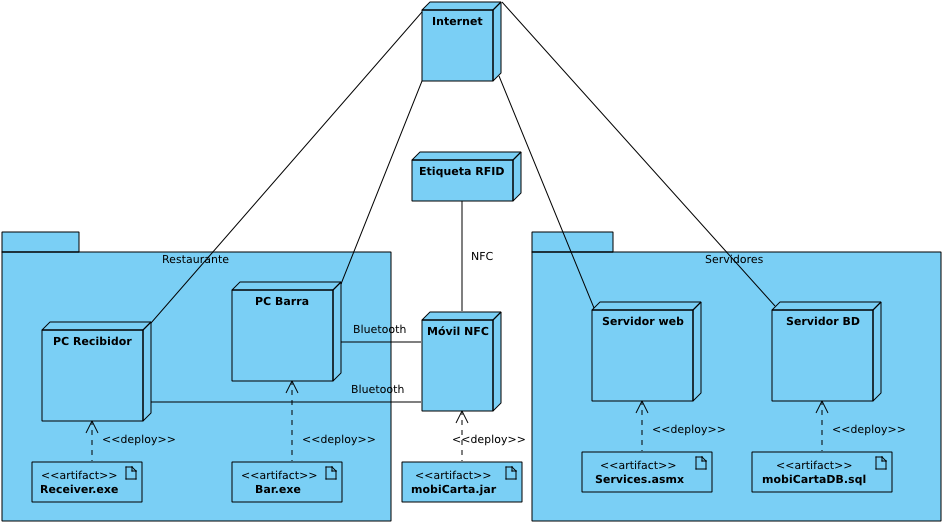
\includegraphics[width=1\textwidth]{deployDiagram.png}
      \caption{Diagrama de despliegue del sistema.}
      \label{fig:deployDiagram}
    \end{center}
  \end{figure}

\section{Iteraciones}
Como ya se explicó en la sección \ref{sec:workingMethodology} (página
\pageref{sec:workingMethodology}) el proyecto sigue un desarrollo de
\emph{prototipado incremental}. Por lo tanto, se basa en la consecución de una
serie de fases o iteraciones, a través de las cuales se van incorporando nuevas
funcionalidades hasta obtener el sistema completo.

A continuación, se profundiza en el contenido de cada una de estas fases:

\subsection{Servicios web y base de datos}
Los servicios web se encargarán de atender las solicitudes de información que
demande la \emph{aplicación de la barra} y la \emph{aplicación del recibidor}.
Para asegurar la persistencia de los datos con los que trabaja el restaurante,
se hará uso de una base de datos.

\subsubsection{Análisis de requisitos}
Los requisitos específicos de los servicios web y de la base de datos son
los siguientes:
\begin{enumerate}
\item Habrá tres tipos de servicios: los que sólo son accedidos por la
aplicación de la \emph{barra}, los que sólo son accedidos por la aplicación
del \emph{recibidor} y los servicios comunes a ambas.
\item Cada servicio ofrecido estará implementado en un método. Los valores
devueltos por el método sólo pueden ser de tipos primitivos (\emph{integer},
\emph{double}, \emph{string}, etc.) por lo que cuando sea necesario devolver
información estructurada se hará uso de cadenas (\emph{string}s) codificadas
en formato \acs{XML}.
\item Entre los servicios que se deben ofrecer están los siguientes:
  \begin{itemize}
  \item Mostrar los tipos de plantilla de restaurante disponibles.
  \item Devolver la descripción de la planta del restaurante elegido.
  \item Añadir una nueva descripción para la planta del restaurante.
  \item Devolver el estado actual de las mesas.
  \item Ubicar a un nuevo cliente en una mesa vacía.
  \item Desubicar a un cliente existente de su mesa.
  \item Devolver el estado actual de los pedidos.
  \item Registrar nuevo pedido.
  \item Cambiar el estado del pedido.
  \item Calcular la factura para una mesa.
  \item Devolver la lista de productos registrados.
  \item Modificar la lista de productos registrados.
  \end{itemize}
\item La aplicación web asegurará la persistencia de los datos con
los que trabaja a través de una base de datos, que se encontrará en la misma
o en distinta máquina que este.
\item La aplicación de los servicios web será la única que pueda acceder a los
datos de la base de datos.
\item La base de datos almacenará tanto los datos estáticos del restaurante 
(como nombre, dirección, NIF, teléfono, etc.), como los datos dinámicos (estado 
de los pedidos, estado de las mesas, etc.).
\item Los datos estáticos definirán la identidad del restaurante, de los
clientes y de los productos que se ofertan.
\item Los datos dinámicos permitirán llevar un seguimiento del estado actual
del restaurante.
\item En resumen, los datos a almacenar serán los siguientes:
  \begin{itemize}
  \item Datos del restaurante (NIF, nombre, teléfono, correo electrónico, IVA, 
  etc.).
  \item Datos de los clientes (DNI, nombre, apellidos, estado, apariciones,
  etc.).
  \item Datos de los productos (nombre, categoría, precio, etc.).
  \item Pedidos registrados durante la sesión.
  \item Descripción de los salones. El salón del restaurante estará
  representado por una serie de objetos que habrán sido definidos por el
  responsable del salón.
  \item Estado de las mesas durante la sesión.
  \item Historial de las facturas.
  \end{itemize}
\end{enumerate}
\newpage
\subsubsection{Diseño e implementación}
Teniendo en cuenta los requisitos definidos en el apartado anterior, se define
el siguiente \textbf{diagrama de casos de uso} (figura \ref{fig:ucdW-phase0}):

  \begin{figure}[H]
    \begin{center}
      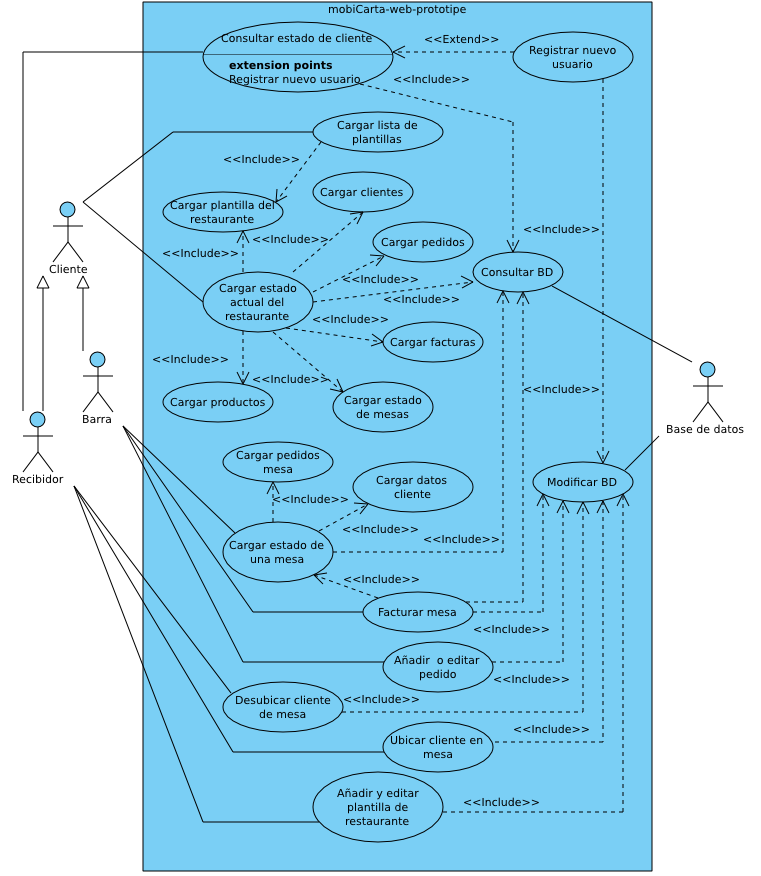
\includegraphics[width=1\textwidth]{ucdW-phase0.png}
      \caption{Diagrama de casos de uso del primer prototipo de la aplicación
      de los servicios web.}
      \label{fig:ucdW-phase0}
    \end{center}
  \end{figure}

Los principales casos de uso definidos en el diagrama (figura
\ref{fig:ucdW-phase0}) son los siguientes:
\begin{itemize}
\item Casos de uso de la \emph{aplicación del recibidor}:
  \begin{itemize}
  \item \textbf{Añadir y editar plantilla de restaurante}. El recibidor
  mandará una petición con la descripción de una nueva plantilla para el 
  restaurante o la modificación de una plantilla existente. El servicio web se 
  encargará de almacenar dicha plantilla en la base de datos.
  \item \textbf{Ubicar cliente en mesa}. Esta petición se producirá cuando
  el recibidor quiera asignar una mesa al cliente que acaba de llegar al
  restaurante. El servicio web actualizará el estado del cliente y de la
  mesa en la base de datos.
  \item \textbf{Desubicar cliente de mesa}. Similar al anterior, en este caso
  cuando el recibidor notifica la marcha de un cliente de su mesa y, por
  consiguiente, del restaurante.
  \end{itemize}
\item Casos de uso de la \emph{aplicación de la barra}:
  \begin{itemize}
  \item \textbf{Añadir o editar pedido}. La aplicación de la barra mandará
  esta petición para que el servicio web actualice la lista de pedidos
  de la base de datos.
  \item \textbf{Cargar estado de una mesa}. Esta petición devolverá los datos
  de la mesa, del cliente que la ocupa y de los pedidos que ha solicitado.
  \item \textbf{Facturar mesa}. En un principio, la aplicación de la barra
  va a ser la única que realice la petición de \emph{facturar mesa}. El
  servicio web cargará: los datos del restaurante (nombre, dirección, IVA, 
  etc.), los de la mesa, los del cliente (nombre, dirección, apariciones, 
  etc.) y los de los pedidos realizados; y generará una factura para dicha
  mesa. La factura generada será almacenada en la base de datos.
  \end{itemize}
\item Casos de uso conjuntos:
  \begin{itemize}
  \item \textbf{Cargar lista de plantillas}. Las aplicaciones de escritorio
  realizarán esta petición para conocer los tipos de plantillas disponibles 
  para dicho restaurante.
  \item \textbf{Cargar estado actual del restaurante}. Al iniciar una jornada
  las aplicaciones de escritorio realizan esta petición para conocer y
  representar el estado actual del restaurante.
  \end{itemize}
\end{itemize}

La forma en la que operan los servicios web es la siguiente:
\begin{itemize}
\item La aplicación se mantiene operativa en espera de peticiones de algún
cliente.
\item Cuando esta llega, recoge los valores de entrada (si los hubiese);
\item los procesa, realizando en algunos casos accesos a alguna base de datos;
\item y devuelve la respuesta obtenida.
\end{itemize}

En este caso, el procesado va a ser bastante simple. La mayor parte de las
peticiones de los clientes van a consistir en una consulta directa a la base
de datos (usando a los servicios web de intermediarios), sin ningún otro
tipo de cálculo intermedio. Si la información obtenida de la base de datos 
no puede ser devuelta a través de ningún tipo primitivo, será almacenada de 
forma temporal en algún objeto, para posteriormente ser devuelta en forma de
cadena (\emph{string}) codificada en \acs{XML}\footnote{El anexo
\ref{chap:xmls} muesta los distintos tipos de objetos definidos en \acs{XML}.}.

Esta forma de operar queda reflejada a través de la definición de estas cuatro 
clases:
\begin{itemize}
\item \textbf{\texttt{Services}}: implementa los servicios web accesibles por 
las aplicaciones del recibidor y de la barra.
\item \textbf{\texttt{DBProxy}}: implementa los métodos que acceden a la base 
de datos. Entre ellos, se encuentra el método \texttt{connect} (para abrir una 
nueva conexión), \texttt{disconnect} (para cerrarla), \texttt{getData} (para 
realizar consultas que devuelven datos) y \texttt{setData} (para realizar
consultas que modifican la base de datos).
\item \textbf{\texttt{SqlProcessor}}: se encarga de construir y ejecutar 
sentencias \acs{SQL} a través de los métodos de \texttt{DBProxy}.
\item \textbf{\texttt{XmlProcessor}}: se encarga de codificar y decodificar las 
cadenas codificadas en \acs{XML}, que envían y reciben los métodos web.
\end{itemize}

%%%% Hay que quitarlo... de momento no
Para la implementación de los servicios web se siguen los procedimientos
descritos en el Anexo \ref{chap:webServices}, definiendo un método web
(\texttt{WebMethod}) por cada caso de uso.

\subsection{\emph{Recibidor} y conexión con servicios web}
La aplicación del \emph{recibidor} se encargará principalmente de registrar a
los clientes que llegan y que salen del restaurante. El prototipo resultante
de esta fase será capaz de registrar la entrada y la salida de clientes que no
hacen uso de la tecnología \acs{NFC}.

\subsubsection{Análisis de requisitos}
Los requisitos específicos de la aplicación del \emph{recibidor} son los
siguientes:
\begin{enumerate}
\item El terminal del recibidor contará con un monitor táctil. Por lo tanto, la 
interfaz de la aplicación debe estar diseñada teniendo en cuenta que no se
dispone de teclado para la entrada de datos.
\item La aplicación contará con un \emph{editor de escenarios} que permita
definir la distribución de los objetos más característicos del restaurante:
  \begin{itemize}
  \item Se podrán definir las posiciones de cada mesa, del espacio ocupado por
  el recibidor y del espacio ocupado por la barra.
  \item Además cada mesa estará definida también por un identificador único y
  por una capacidad.
  \item Cada tipo de objeto será representado por un color.
  \item El editor permitirá cargar y guardar escenarios. Los escenarios serán
  almacenados en la base de datos a través del servicio web correspondiente.
  \end{itemize}
\item Al iniciar la ejecución, el usuario tendrá dos opciones:
\emph{iniciar una nueva jornada}, que reseteará los datos dinámicos
correspondientes al estado anterior del restaurante (pedidos pendientes y
estado de las mesas); o \emph{iniciar una jornada existente}, que cargará
estos datos.
\item Al \emph{iniciar una nueva jornada}, el usuario elegirá la plantilla de
restaurante que va a utilizar para representar la distribución actual de los
objetos que hay en él.
\item El estado del restaurante se representará con un mapa similar al mostrado
en el \emph{editor de escenarios}, con la salvedad de que las mesas aparecerán
de un color distinto según su estado.
\item Cada mesa se encontrará en uno de los siguientes estados:
  \begin{itemize}
  \item \textbf{Libre}. Cuando la mesa no está ocupada por ningún cliente.
  \item \textbf{Ocupada}. Cuando la mesa está ocupada por un cliente.
  \item \textbf{Cobrada}. Cuando la mesa está ocupada por un cliente que ya
  ha pagado. Esto implica que el cliente puede abandonar el restaurante
  cuando quiera y que va a dejar la mesa libre.
  \end{itemize}
\item Cada cliente estará representado por un identificador único.
\item Para registrar el ingreso de un nuevo cliente, la aplicación mostrará
las mesas que este puede ocupar, teniendo en cuenta el número de comensales que
son y la capacidad de las mesas.
\item Para confirmar la salida de un cliente, la aplicación sólo dejará
desocupar las mesas que hayan pagado sus pedidos o las mesas cuyos clientes
se vayan sin consumir nada.
\item Se contará con un editor de parámetros del restaurante, que permitirá
definir los datos de la empresa (nombre, dirección, etc.) o las condiciones
por las cuales se aplican descuentos, entre otras; y con un visor de clientes,
que muestre la información de los clientes almacenados por el sistema.
\end{enumerate}
\newpage
\subsubsection{Diseño e implementación}
Teniendo en cuenta el análisis de requisitos realizado anteriormente, el
\textbf{diagrama de casos de uso} del prototipo de la aplicación del
\emph{recibidor} quedaría de la siguiente forma (figura \ref{fig:ucdR-phase1}):

  \begin{figure}[H]
    \begin{center}
      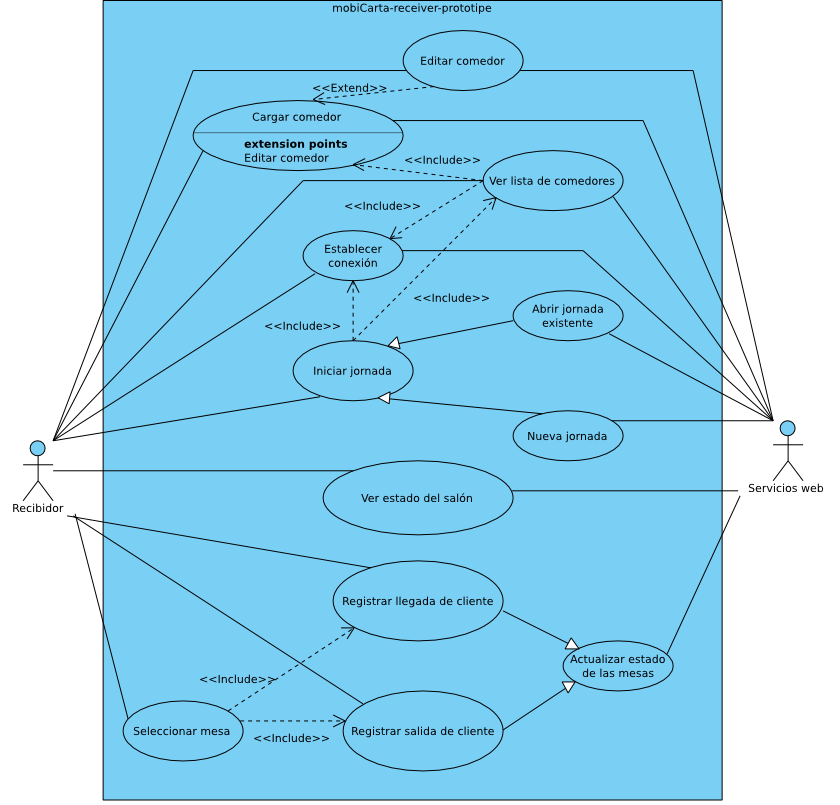
\includegraphics[width=1\textwidth]{ucdR-phase1.png}
      \caption{Diagrama de casos de uso del primer prototipo de la aplicación
      del \emph{recibidor}.}
      \label{fig:ucdR-phase1}
    \end{center}
  \end{figure}

Los principales casos de uso que muestra el diagrama (figura
\ref{fig:ucdR-phase1}) son los siguientes:
\begin{itemize}
\item \textbf{Nueva jornada}. Cuando el \emph{recibidor} quiere iniciar una
nueva jornada (``desde cero''), le pide al \emph{servicio web} que le mande 
una lista con los salones que previamente ha diseñado. De entre todos ellos
elige el que se adapte a la distribución actual de los objetos en el
restaurante y le pide al \emph{servicio web} que le mande la distribución del
salón elegido para cargarlo en pantalla. Una vez cargado, el \emph{recibidor}
vuelve a comunicarse con el \emph{servicio web} para decirle que \emph{resetee}
los valores almacenados de la jornada anterior. La figura \ref{fig:sdR1-phase1}
(página \pageref{fig:sdR1-phase1}) muestra el \textbf{diagrama de secuencia} 
de este caso de uso.

\item \textbf{Abrir jornada existente}. Este caso de uso es similar al
anterior, con la salvedad de que, aquí no se elige el salón a
utilizar (se coge el salón de la jornada anterior). Además, tampoco se
\emph{resetean} los valores almacenados durante dicha jornada. La figura
\ref{fig:sdR2-phase1} (página \pageref{fig:sdR2-phase1}) muestra el
\textbf{diagrama de secuencia} de este caso de uso.

\item \textbf{Registrar llegada de cliente}. Este caso de uso hace referencia
a la acción de registrar un nuevo cliente de forma manual
(\emph{no-\acs{NFC}}). Cuando se confirma una nueva llegada, se
genera un identificador único que se le asigna al cliente entrante.
Este identificador tendrá la siguiente forma: un prefijo, 'C'; seguido del
año, mes, día, minuto y segundo en el que se produce el registro. Por ejemplo,
el cliente $C20120720214850$ habrá llegado a las $21:48:50$ del día $20$ de
\emph{Julio} de $2012$. A continuación, el cliente introduce el número de
comensales que son. La aplicación (a través del \emph{servicio web})
comprobará las mesas que están disponibles y que tienen una capacidad
suficiente y las mostrará por pantalla. Por último, se marcará una de las
mesas candidatas y se formalizará con ello el ingreso. Nuevamente el
\emph{servicio web} actualizará el estado de las mesas teniendo en cuenta el
nuevo ingreso. La figura \ref{fig:sdR3-phase1} (página
\pageref{fig:sdR3-phase1}) muestra el \textbf{diagrama de secuencia} de este
caso de uso.

\item \textbf{Registrar salida de cliente}. Para registrar la salida de un
cliente (\emph{normal} o \emph{\acs{NFC}}), simplemente se selecciona la
opción de \emph{Cliente se va}. La aplicación recurre al \emph{servicio web}
para actualizar el estado de las mesas y con ello representa cuáles son las
susceptibles de quedarse vacías. En este caso, las mesas candidatas son
aquellas en las que el cliente ha pagado la cuenta. A continuación, se marca
cuál es la mesa que va a ser abandonada y se pulsa \emph{Aceptar}. Finalmente,
la aplicación avisa al \emph{servicio web} acerca de la mesa que ha quedado
libre y este actualiza el estado del salón. La figura \ref{fig:sdR4-phase1}
(página \pageref{fig:sdR4-phase1}) representa el \textbf{diagrama de secuencia}
del caso de uso \emph{registrar salida de cliente}.
\end{itemize}

  \begin{sidewaysfigure}[hp]
    \begin{center}
      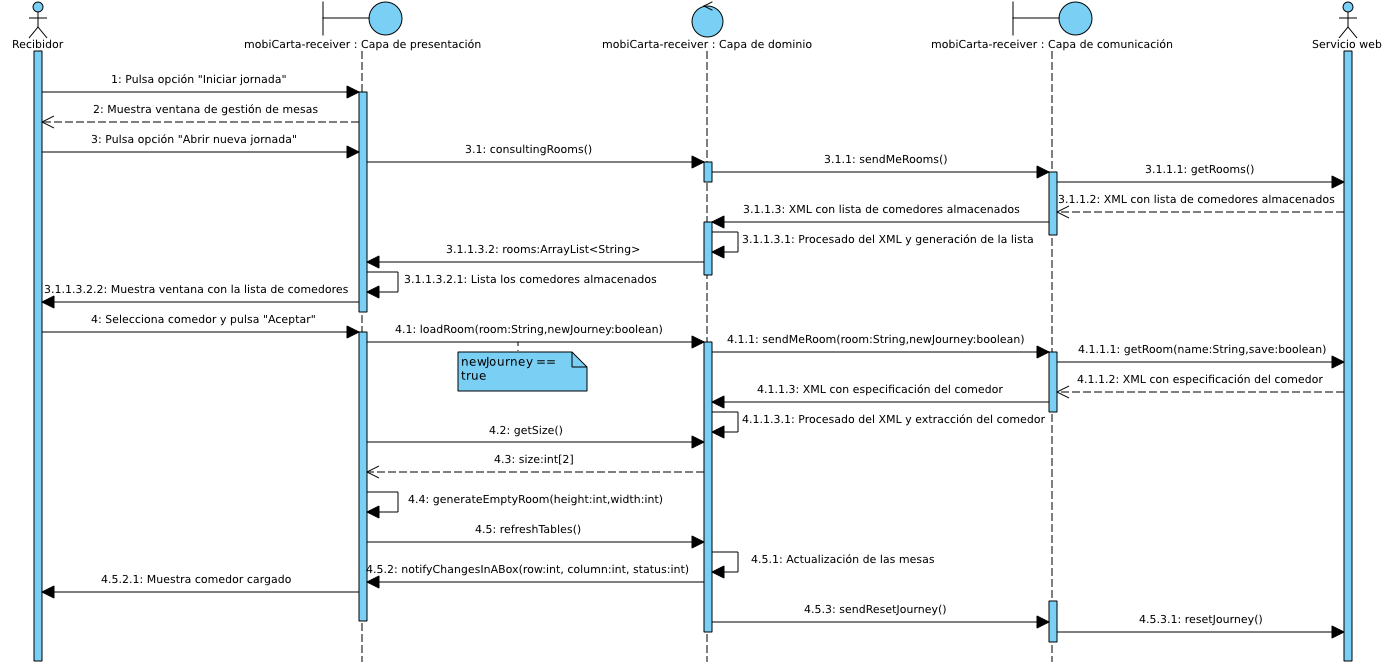
\includegraphics[width=1\textwidth]{sdR1-phase1.png}
      \caption{Diagrama de secuencia del caso de uso \emph{iniciar nueva
      jornada}.}
      \label{fig:sdR1-phase1}
    \end{center}
  \end{sidewaysfigure}

  \begin{sidewaysfigure}[hp]
    \begin{center}
      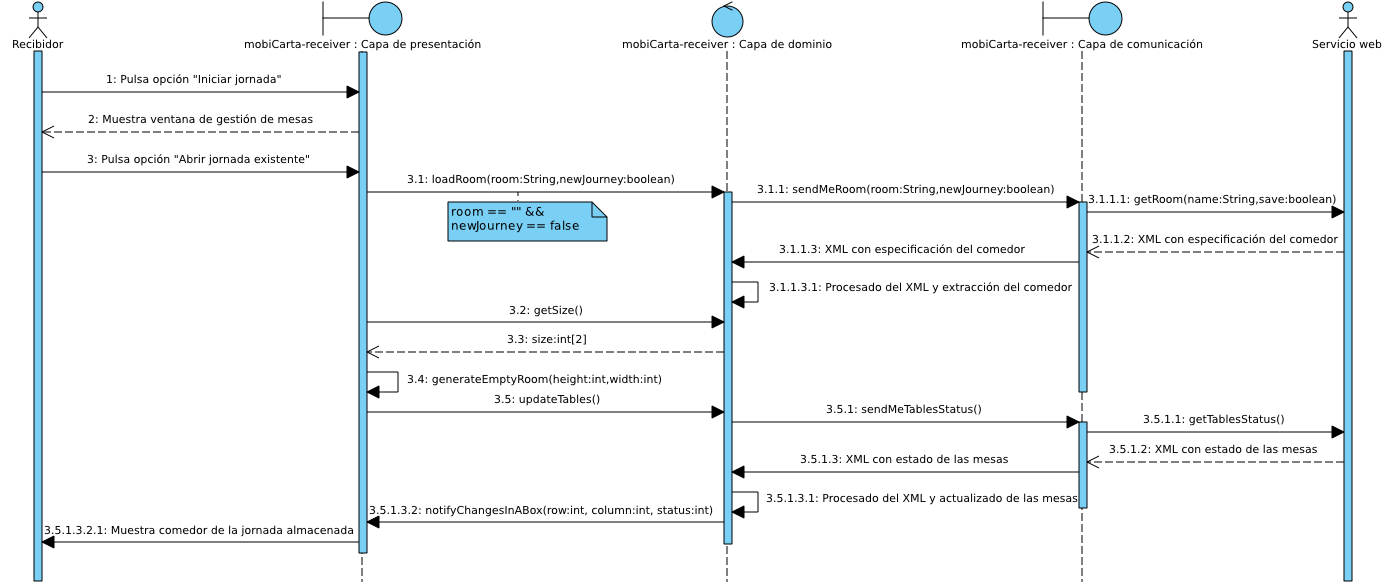
\includegraphics[width=1\textwidth]{sdR2-phase1.png}
      \caption{Diagrama de secuencia del caso de uso \emph{iniciar jornada
      existente}.}
      \label{fig:sdR2-phase1}
    \end{center}
  \end{sidewaysfigure}

  \begin{sidewaysfigure}[hp]
    \begin{center}
      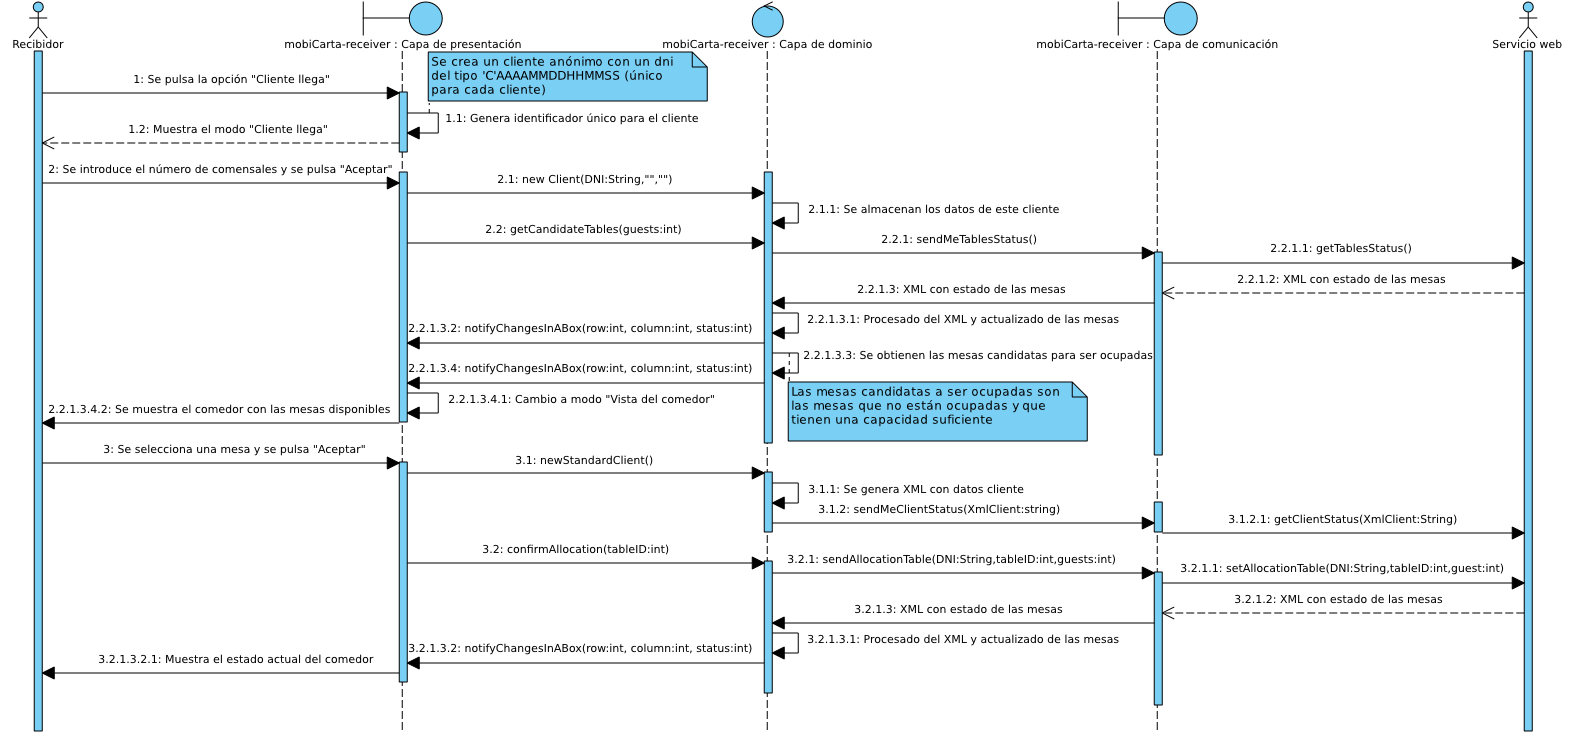
\includegraphics[width=1\textwidth]{sdR3-phase1.png}
      \caption{Diagrama de secuencia del caso de uso \emph{registrar llegada
      de cliente}.}
      \label{fig:sdR3-phase1}
    \end{center}
  \end{sidewaysfigure}

  \begin{sidewaysfigure}[hp]
    \begin{center}
      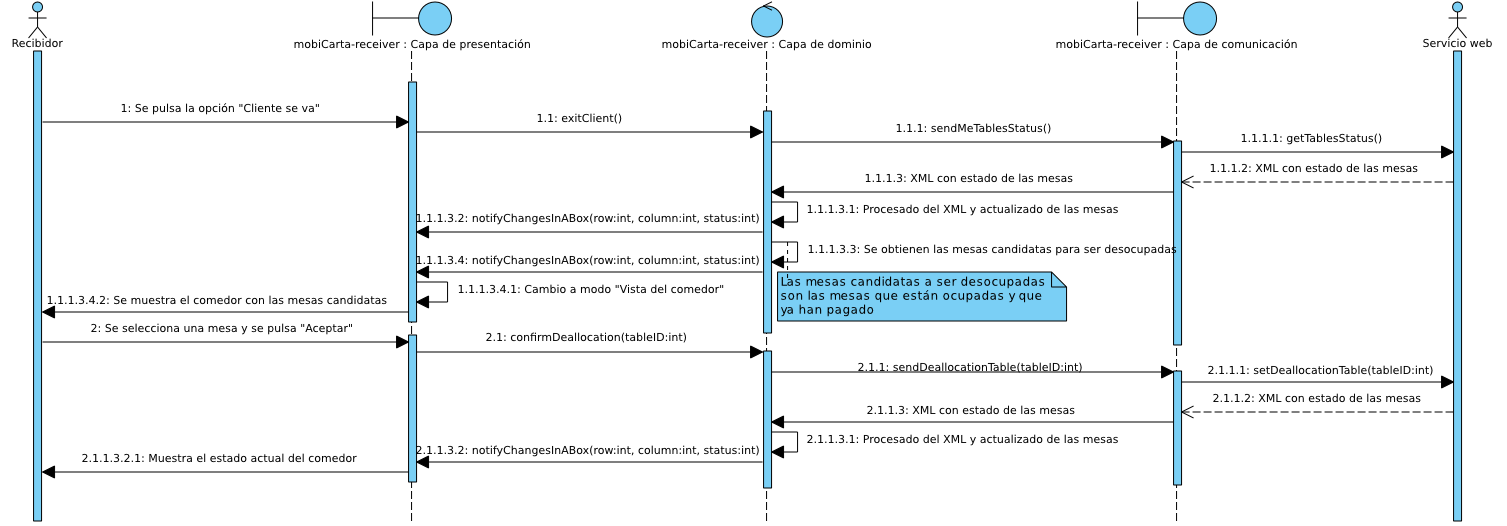
\includegraphics[width=1\textwidth]{sdR4-phase1.png}
      \caption{Diagrama de secuencia del caso de uso \emph{registrar salida
      de cliente}.}
      \label{fig:sdR4-phase1}
    \end{center}
  \end{sidewaysfigure}
\newpage
A partir de los diagramas de casos de uso y de los diagramas de secuencia se
diseña el \textbf{diagrama de clases} del prototipo del recibidor (de esta
fase) (figura \ref{fig:cdR-phase1}, página \pageref{fig:cdR-phase1}):

  \begin{sidewaysfigure}[hp]
    \begin{center}
      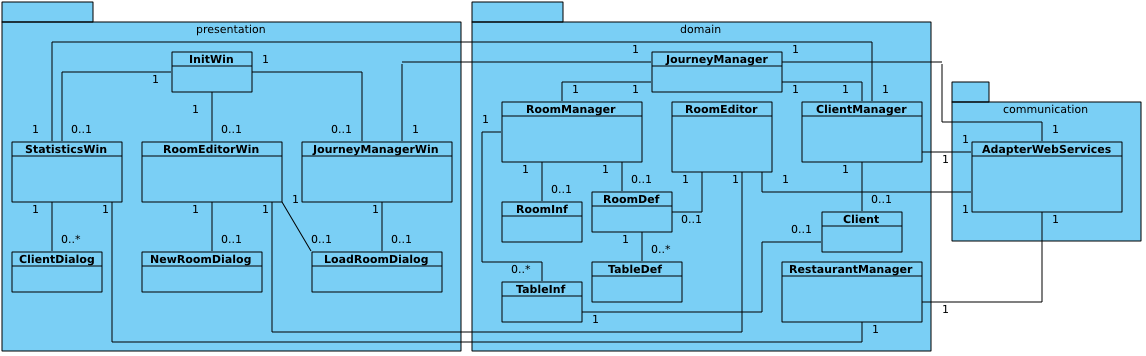
\includegraphics[width=1\textwidth]{cdR-phase1.png}
      \caption{Diagrama de clases del prototipo del recibidor (Fase 2).}
      \label{fig:cdR-phase1}
    \end{center}
  \end{sidewaysfigure}

Las clases de este prototipo son las siguientes:
\begin{itemize}
\item El paquete \texttt{presentation} contiene las clases que implementan
la \acs{GUI} de la aplicación:
  \begin{itemize}
  \item \textbf{\texttt{InitWin}}: implementa la ventana inicial, a través de 
  la cual se accede a las demás opciones de la aplicación.
  \item \textbf{\texttt{JouneyManagerWin}}: describe la ventana principal de la
  aplicación, desde la cual se gestiona el trascurso de una jornada de trabajo.
  Permite registrar la entrada y salida de clientes; y mantiene una vista
  actualizada del estado del restaurante.
  \item \textbf{\texttt{RoomEditorWin}}: permite crear, editar y guardar las
  plantillas del restaurante. Cada plantilla describe visualmente una posible
  distribución de objetos: mesas, recibidor y barra, dentro del restaurante.
  \item \textbf{\texttt{StatisticsWin}}: permite consultar el estado 
  actualizado de los clientes del restaurante. Además, también permite editar   
  la información referida al restaurante: nombre, dirección, contacto, IVA,
  etc.
  \item \textbf{\texttt{ClientDialog}}, \textbf{\texttt{NewRoomDialog}} y
  \textbf{\texttt{LoadRoomDialog}} implementan ventanas emergentes auxiliares a 
  las clases de las que dependen.
  \end{itemize}
\item El paquete \texttt{domain} contiene las clases que gestionan la 
información que entra y sale de la aplicación:
  \begin{itemize}
  \item \textbf{\texttt{JourneyManager}}: gestiona todas las operaciones 
  implicadas en el desarrollo de una jornada de trabajo en el restaurante.
  \item \textbf{\texttt{RoomManager}}: implementa las operaciones relacionadas 
  con la actualización del estado de la plantilla del restaurante y, por
  extensión de sus mesas.
  \item \textbf{\texttt{ClientManager}}: gestiona los datos de los clientes 
  implicados en una interacción (cliente llega, cliente se va, etc.).
  \item \textbf{\texttt{RoomEditor}}: implementa la lógica del editor de 
  plantillas (\texttt{RoomEditorWin}).
  \item \textbf{\texttt{RestaurantManager}}: gestiona los datos mostrados por
  \texttt{StatisticsWin}.
  \end{itemize}
Las demás clases definen tipos de objetos:
  \begin{itemize}
  \item \textbf{\texttt{Client}}: DNI, nombre, apellidos y dirección de un 
  cliente del restaurante.
  \item \textbf{\texttt{RoomInf}}: resume las características de una plantilla 
  de restaurante (nombre, altura, anchura, número de mesas y capacidad).
  \item \textbf{\texttt{TableInf}}: almacena la información detallada de una 
  mesa (identificador, capacidad y ubicación) y su estado (cliente que la ocupa 
  y número de comensales).
  \item \textbf{\texttt{RoomDef}}: define las características detalladas de una
  plantilla de restaurante (nombre, altura, anchura y ubicación de cada uno
  de los objetos).
  \item \textbf{\texttt{TableDef}}: define las características de cada una de 
  las mesas almacenadas por un objeto \texttt{RoomDef} (identificador, capacidad
  y ubicación).
  \end{itemize} 
\item El paquete \texttt{communication} contiene un sólo método,
\textbf{\texttt{AdapterWebServices}}. Este método se encarga de realizar las 
peticiones a los servicios web y de recoger sus posibles respuestas.
\end{itemize}

\subsection{\emph{Barra} y conexión con servicios web}
La aplicación de la \emph{barra} se encargará principalmente de gestionar el
estado de los pedidos de los clientes. El prototipo resultante de esta
iteración será capaz de realizar todas las funcionalidades definidas para
los \emph{clientes normales} (ver apartado \emph{Los clientes},
subsección \ref{subsubsec:clients}, página \pageref{subsubsec:clients}).

\subsubsection{Análisis de requisitos}
Los requisitos específicos de la aplicación de la \emph{barra} son los
siguientes:
\begin{enumerate}
\item El terminal de la barra contará con un monitor táctil, por lo que la
aplicación debe estar diseñada teniendo en cuenta que la mayor parte de las
interacciones se realizarán sin hacer uso del teclado.
\item La aplicación contará con un \emph{editor de productos} que permita
definir las características de los productos que hay a la venta:
  \begin{itemize}
  \item Los productos estarán clasificados por categorías, por lo que el
  editor también podrá eliminar, crear y editar nuevas categorías.
  \item El producto quedará identificado por su nombre.
  \item Además del nombre y la categoría, cada producto tendrá otros atributos
  como: el precio, el número de unidades que hay que pedir para obtener un
  descuento (si lo tuviese), el \% de dicho descuento y un atributo
  \emph{booleano} que determine si el producto aparecerá como visible o no
  visible a la hora de realizar pedidos.
  \end{itemize}
\item Como ocurría con la aplicación del \emph{recibidor}, la aplicación de la
\emph{barra} también tiene dos opciones: \emph{iniciar una nueva jornada} e
\emph{iniciar una jornada existente}. El funcionamiento es el mismo que las
funciones homónimas ya comentadas.
\item El estado del restaurante se muestra de forma similar a como lo hace
la aplicación del \emph{recibidor}, con la salvedad de que ahora las mesas
tienen otros estados:
  \begin{itemize}
  \item \textbf{Libre}. La mesa no está ocupada por ningún cliente.
  \item \textbf{Ocupada}. La mesa está ocupada por un cliente que no ha
  realizado aún ningún pedido.
  \item \textbf{Esperando}. El cliente de dicha mesa ha realizado un pedido y
  este aún no ha sido entregado.
  \item \textbf{Atendida}. Todos los pedidos que ha hecho el cliente de esta
  mesa han sido atendidos.
  \item \textbf{Cobrada}. Los pedidos de esta mesa han sido cobrados, pero el
  cliente aún no la ha abandonado.
  \end{itemize}
\item La aplicación debe tener la funcionalidad para anotar pedidos similar a 
las ya vistas en otros gestores de restaurantes (ver figuras
\ref{fig:productsPanel}, \ref{fig:productsPanel2} y \ref{fig:productsList},
página \pageref{fig:productsPanel}).
\item La aplicación mostrará una lista con todos los pedidos que han sido
realizados durante la sesión.
\item Los pedidos podrán encontrarse en uno de estos estados:
  \begin{itemize}
  \item \textbf{No atendido}. Se ha tomado nota del pedido pero nadie se está
  haciendo cargo de él.
  \item \textbf{Atendido}. En caso de que el producto tenga que ser elaborado
  (por un cocinero, por ejemplo), este estado determina que el plato está
  siendo cocinado.
  \item \textbf{Servido}. Cuando el producto ha llegado a su destinatario, el
  estado del producto debe cambiarse a \emph{servido}.
  \item \textbf{Detenido}. En caso de producirse alguna incidencia con el
  pedido (por ejemplo, falta alguna materia prima para elaborar
  el plato pero se repondrá en breve), es conveniente contar con un estado
  de \emph{excepción}.
  \item \textbf{Cobrado}. Para identificar que los pedidos de esa mesa ya han
  sido cobrados.
  \end{itemize}
\item La aplicación podrá mostrar la situación de una mesa en concreto: quién
la ocupa, en qué estado se encuentra, cuáles son sus pedidos, cuál es el
estado de dichos pedidos, etc.
\item Cuando todos los pedidos de una mesa han sido atendidos, se dará la
opción de \emph{facturar} la mesa. Los datos personales suministrados por el
cliente y los datos fiscales de la empresa almacenados en la base de datos
servirán para generar la factura.
\item Se contará con un visor que muestre el historial de facturas cobradas y
el de pedidos atendidos.
\end{enumerate}
\newpage
\subsubsection{Diseño e implementación}
Teniendo en cuenta el análisis de requisitos realizado anteriormente, el
\textbf{diagrama de casos de uso} del prototipo de la aplicación de la
\emph{barra} queda de la siguiente forma (figura \ref{fig:ucdB-phase2}).

  \begin{figure}[H]
    \begin{center}
      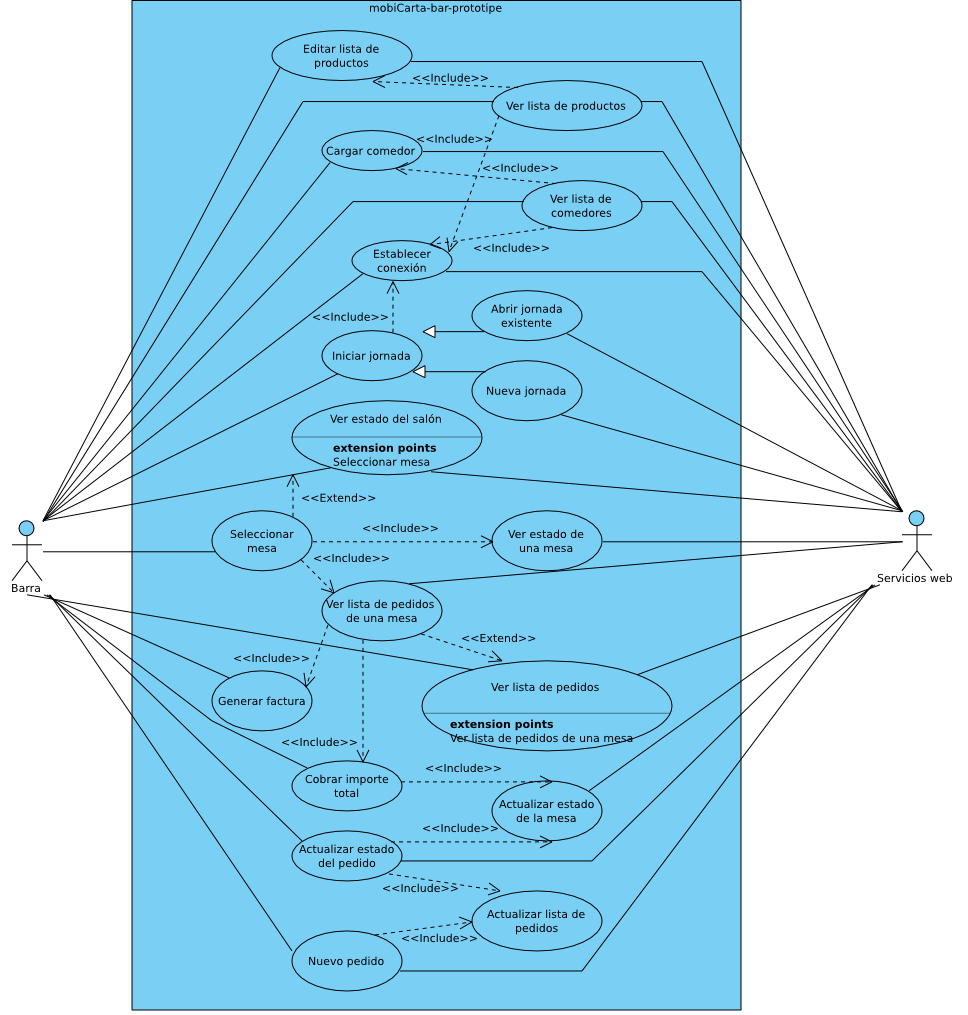
\includegraphics[width=1\textwidth]{ucdB-phase2.png}
      \caption{Diagrama de casos de uso del primer prototipo de la aplicación
      de la \emph{barra}.}
      \label{fig:ucdB-phase2}
    \end{center}
  \end{figure}

Los casos de uso más característicos de la aplicación de la \emph{barra} son
los siguientes:
\begin{itemize}
\item Los casos de uso \textbf{Nueva jornada} y \textbf{Abrir jornada
existente} son exactamente iguales que los ya explicados en la aplicación
del \emph{recibidor}. Por lo tanto, los diagramas de secuencia van a ser 
idénticos a los de las figuras \ref{fig:sdR1-phase1} (página
\pageref{fig:sdR1-phase1}) y \ref{fig:sdR2-phase1} (página
\pageref{fig:sdR2-phase1}), respectivamente.
\item \textbf{Ver estado de una mesa}. Durante una jornada activa se tiene
la posibilidad de observar el estado actual del salón. Para ello simplemente
hay que seleccionar la opcion \emph{Mostrar salón}. Para conocer el estado
actualizado del salón, la aplicación echa mano del \emph{servicio web}.
La vista del salón da la posibilidad de seleccionar las mesas ocupadas. Como
ocurre con el estado del salón, la aplicación recurre nuevamente al
\emph{servicio web} para conocer el estado actualizado de la mesa seleccionada.
Esta información incluye: estado de la mesa, cliente que la ocupa, número
de comensales y los pedidos (y su estado) que ha realizado. La figura
\ref{fig:sdB1-phase2} (página \pageref{fig:sdB1-phase2}), muestra el
\textbf{diagrama de secuencia} de este caso de uso.

\item \textbf{Nuevo pedido}. Al seleccionar el botón de \emph{añadir pedido}
la aplicación carga una lista con las mesas activas y otra lista con los
productos disponibles. Para asignar un pedido a una mesa: en primer lugar, se
selecciona la mesa de destino; a continuación, se selecciona la categoría
del producto que se pretende añadir; después, se elige la cantidad de
productos que van a añadirse; y por último, se selecciona el producto y se
pulsa \emph{añadir}. La lista de productos generada se le asignará a la mesa
al pulsar \emph{Aceptar}. Este nuevo pedido se envía (en formato \acs{XML})
al \emph{servicio web}. La figura \ref{fig:sdB2-phase2} (página
\pageref{fig:sdB2-phase2}) muestra el \textbf{diagrama de secuencia} de dicho
caso de uso.

\item \textbf{Actualizar el estado de un pedido}. Para cambiar el estado de
un pedido, hay que seleccionarlo en la lista de pedidos y pulsar después uno
de los estados disponibles (\emph{No atendido}, \emph{Atendido},
\emph{Servido}, o \emph{Detenido}). El pedido cambiará de color y se informará
al \emph{servicio web} que dicho cambio.
La figura \ref{fig:sdB3-phase2} (página \pageref{fig:sdB3-phase2}) muestra
un \textbf{diagrama de secuencia} en el que, primero, se cambia el estado de
un producto de \emph{No atendido} a \emph{Atendido}, para informar de que
el pedido está siendo elaborado; y posteriormente se cambia de \emph{Atendido}
a \emph{Servido}, para indicar que el pedido ha sido entregado a la mesa.

\item \textbf{Generar factura} y  \textbf{Cobrar importe total}. Para
facturar una mesa, primero hay que asegurarse de que todos sus pedidos han
sido servidos. Después hay que situarse en la \emph{vista de esa mesa}.
Al pulsar la opción \emph{Facturar}, la aplicación buscará, entre las facturas
generadas, si ha generado la de esa mesa. En caso de no encontrarla recurrirá
al \emph{servicio web}, que es el que en verdad genera las facturas. El
\emph{servicio web} devolverá un \acs{XML} con la factura para esa mesa y la 
aplicación se encargará de decodificarla para crear un objeto de tipo
\emph{Bill}, lo almacenará con el resto de facturas generadas y compondrá
una ventana emergente con los datos de la factura. Una de las opciones de
esa ventana emergente será la de \emph{Pagado}. Con ella se confirmará que
el importe que debe la mesa se ha abonado. La aplicación marcará los
pedidos para esa mesa como \emph{Pagado}s y se informará al \emph{servicio
web} de esta operación. El \emph{servicio web} marcará también esos pedidos
como \emph{Pagado}s, los sacará de la tabla \emph{Orders} y los meterá en
\emph{Historical} y devolverá un \acs{XML} con el nuevo estado del
restaurante. La figura \ref{fig:sdB4-phase2} (página \pageref{fig:sdB4-phase2})
muestra el \textbf{diagrama de secuencia} de estos dos casos de uso.
\end{itemize}

  \begin{sidewaysfigure}[hp]
    \begin{center}
      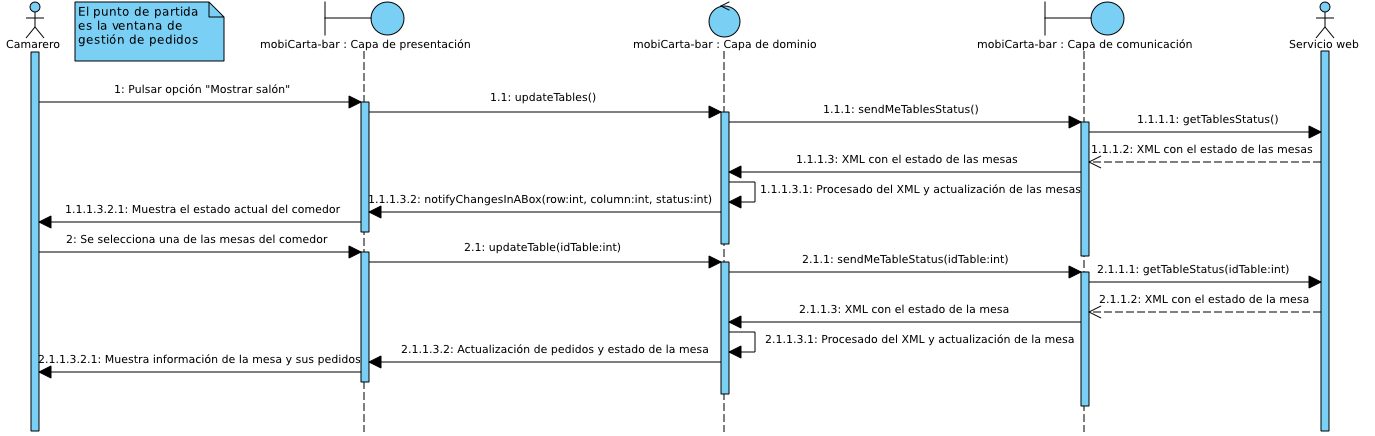
\includegraphics[width=1\textwidth]{sdB1-phase2.png}
      \caption{Diagrama de secuencia del caso de uso \emph{Ver estado de
      una mesa}.}
      \label{fig:sdB1-phase2}
    \end{center}
  \end{sidewaysfigure}

  \begin{sidewaysfigure}[hp]
    \begin{center}
      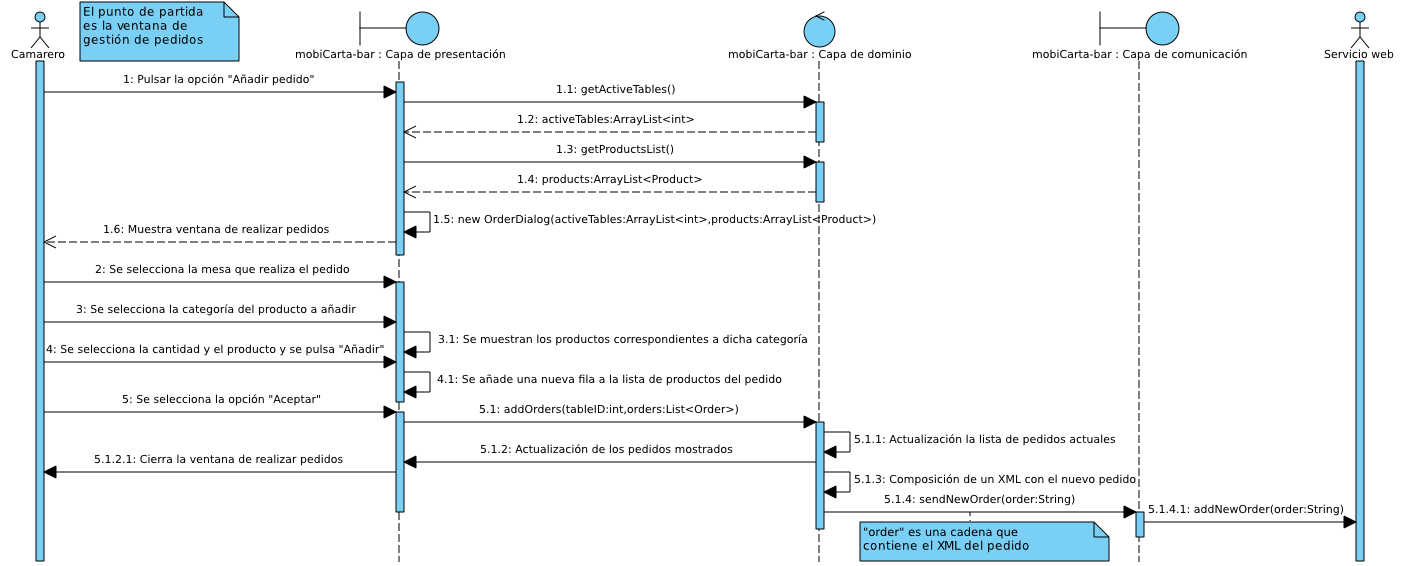
\includegraphics[width=1\textwidth]{sdB2-phase2.png}
      \caption{Diagrama de secuencia del caso de uso \emph{añadir un nuevo
      pedido (manual)}.}
      \label{fig:sdB2-phase2}
    \end{center}
  \end{sidewaysfigure}

  \begin{sidewaysfigure}[hp]
    \begin{center}
      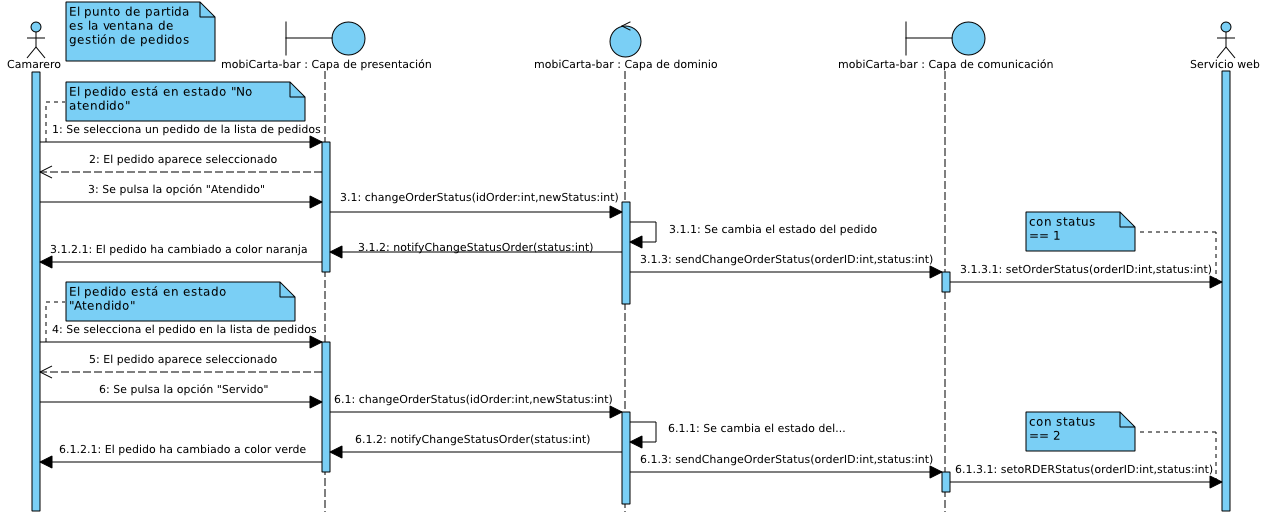
\includegraphics[width=1\textwidth]{sdB3-phase2.png}
      \caption{Diagrama de secuencia del caso de uso \emph{actualizar
      estado de un pedido} de \emph{No atendido} a \emph{Servido}.}
      \label{fig:sdB3-phase2}
    \end{center}
  \end{sidewaysfigure}

  \begin{sidewaysfigure}[hp]
    \begin{center}
      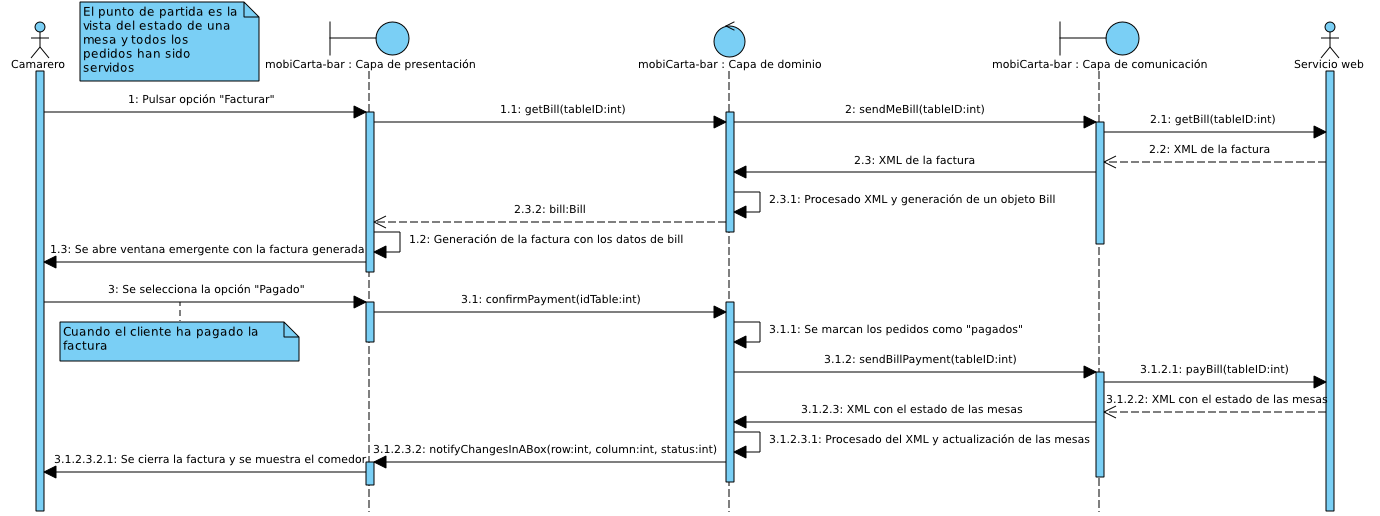
\includegraphics[width=1\textwidth]{sdB4-phase2.png}
      \caption{Diagrama de secuencia del caso de uso \emph{generar factura}
      y \emph{cobrar importe total}.}
      \label{fig:sdB4-phase2}
    \end{center}
  \end{sidewaysfigure}

Haciendo uso de los diagramas de casos de uso y de secuencia se
diseña el diagrama de clases del prototipo de la aplicación de la barra
(figura \ref{fig:cdB-phase2}, página \pageref{fig:cdB-phase2}):

  \begin{sidewaysfigure}[hp]
    \begin{center}
      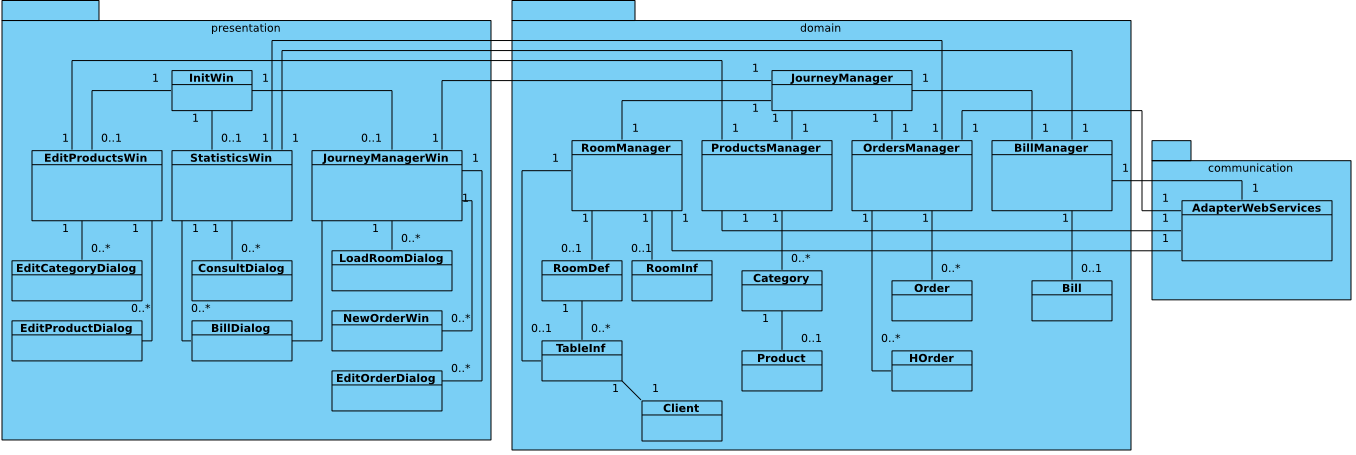
\includegraphics[width=1\textwidth]{cdB-phase2.png}
      \caption{Diagrama de clases del prototipo de la aplicación de la barra
      (Fase 3).}
      \label{fig:cdB-phase2}
    \end{center}
  \end{sidewaysfigure}

Las clases de este prototipo son las siguientes:
\begin{itemize}
\item El paquete \texttt{presentation} contiene las clases que implementan
la \acs{GUI} del prototipo:
  \begin{itemize}
  \item \textbf{\texttt{JourneyManagerWin}}: cumple el mismo cometido que la 
  clase homónima del prototipo del recibidor salvo que, en este caso, se encarga
  de gestionar los pedidos de los clientes y su facturación.
  \item \textbf{\texttt{EditProductsWin}}: implementa un editor que permite 
  añadir, editar o borrar productos de la lista de productos del restaurante.
  \item \textbf{\texttt{StatisticsWin}}: permite consultar el histórico de 
  facturas emitidas y el histórico de pedidos cobrados.
  \item \texttt{\textbf{EditCategoryDialog}} y
  \textbf{\texttt{EditProductDialog}}: forman
  parte del editor de productos (\texttt{EditProductsWin}) y permiten editar
  o crear nuevas categorías y editar o crear nuevos productos, respectivamente.
  \item \textbf{\texttt{ConsultDialog}}: implementa una ventana emergente 
  dependiente de \texttt{StatisticsWin}, a través de la cual se elige el tamaño 
  (número de elementos) y el orden (ascendente o descendente) de la búsqueda de 
  facturas o de la búsqueda de pedidos ya cobrados.
  \item \textbf{\texttt{BillDialog}}: ventana emergente que muestra los 
  elementos habituales de una factura: datos de la empresa, datos del cliente, 
  pedidos realizados, \% de descuentos, \% de IVA e importe total, entre otros.
  \item \textbf{\texttt{NewOrderWin}} y \textbf{\texttt{EditOrderDialog}}: 
  ventanas emergentes que permiten añadir y editar pedidos, respectivamente.
  \end{itemize}
\item El paquete \texttt{domain} contiene las clases que implementan la lógica
del prototipo:
  \begin{itemize}
  \item \textbf{\texttt{ProductsManager}}: se encarga de gestionar las 
  operaciones relacionadas con la carga y modificación de la lista de productos 
  del restaurante.
  \item \textbf{\texttt{OrdersManager}}: implementa la lógica que permite la 
  gestión de los pedidos realizados durante una jornada de trabajo.
  \item \textbf{\texttt{BillManager}}: permite decodificar las facturas creadas 
  por los servicios web para, posteriormente, representarlas en una ventana de 
  tipo \texttt{BillDialog}.
  \item \textbf{\texttt{Product}}: almacena la información de un producto 
  (nombre, categoría, precio, descripción y descuentos).
  \item \textbf{\texttt{Category}}: define una categoría de productos. Está 
  compuesta por un nombre y la lista de objetos de tipo \texttt{Product} de esa
  categoría.
  \item \textbf{\texttt{Order}}: almacena la información referida a un pedido:
  identificador, producto, cantidad, fecha, mesa de destino y estado del
  pedido en ese momento (\emph{no atendido}, \emph{atendido}, \emph{servido}
  o \emph{detenido}).
  \item \textbf{\texttt{HOrder}}: representa la información de un pedido que 
  forma parte del historial de pedidos del restaurante. Es decir, un pedido que 
  ya ha sido cobrado (fecha, producto, cantidad y cliente que lo consumió).
  \item \textbf{\texttt{Bill}}: almacena la información referida a una factura:
  número de factura, datos del cliente, datos de la empresa, pedidos, importe
  total, etc.
  \end{itemize}
\item Las clases \textbf{\texttt{InitWin}}, \textbf{\texttt{JourneyManager}},
\textbf{\texttt{RoomManager}}, \textbf{\texttt{RoomDef}},
\textbf{\texttt{RoomInf}}, \textbf{\texttt{TableInf}},
\textbf{\texttt{LoadRoomDialog}} y \textbf{\texttt{AdapterWebServices}} 
implementan una funcionalidad similar a las clases homónimas del prototipo del 
recibidor.
\end{itemize}

Una vez definidas las funcionalidades básicas (no \acs{NFC}) de las
aplicaciones de escritorio (\emph{barra} y \emph{recibidor}) y de los servicios 
web, así como también de los datos con los que trabajan; se ha definido la 
\textbf{base de datos} del sistema.

  \begin{figure}[H]
    \begin{center}
      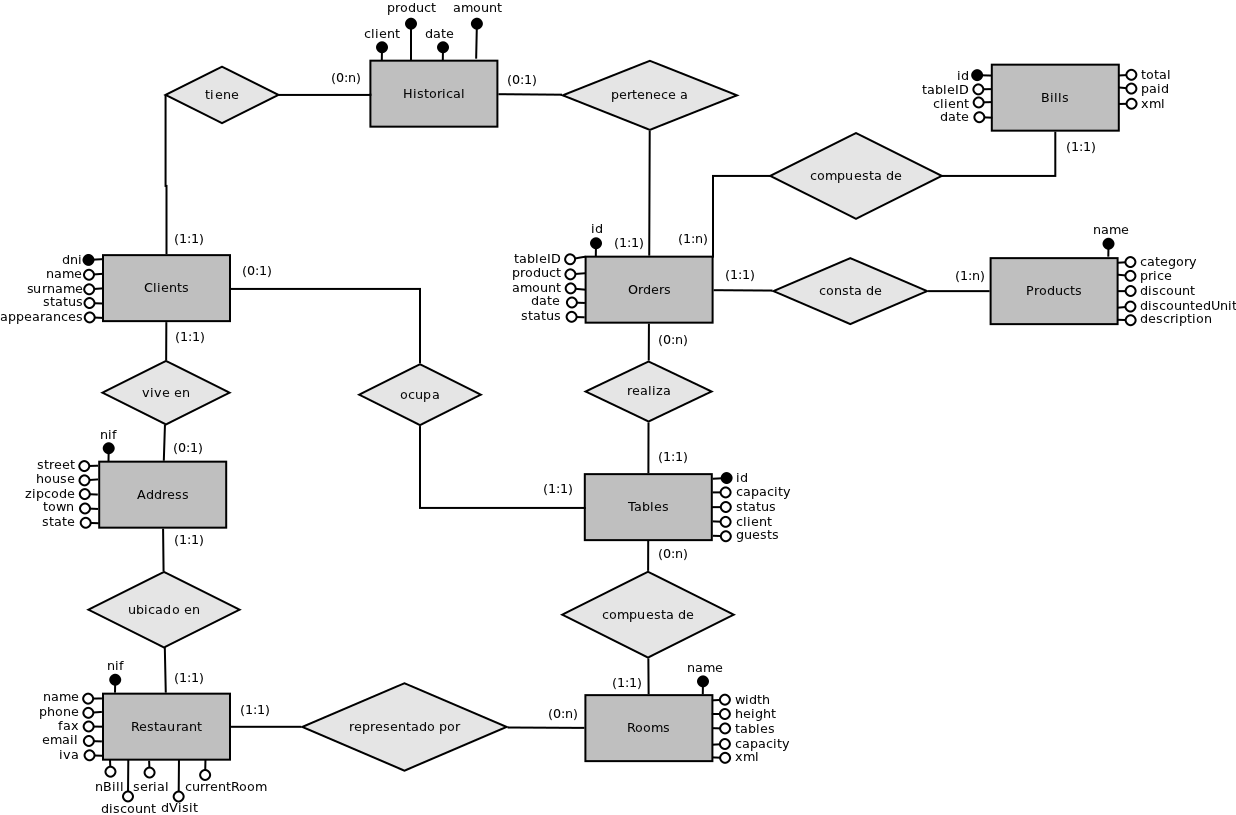
\includegraphics[width=1.1\textwidth]{erdDB.png}
      \caption{Diagrama entidad-relación de la base de datos del sistema.}
      \label{fig:erdDB}
    \end{center}
  \end{figure}

La figura \ref{fig:erdDB} (página \pageref{fig:erdDB}) muestra el
\textbf{diagrama de entidad-interrelación} de la base de datos. En ella pueden 
observarse los siguientes elementos:
\begin{itemize}
\item \textbf{\texttt{Restaurant}}: almacena la información que define al 
restaurante (NIF, nombre, información de contacto, IVA aplicado, descuentos por 
fidelidad, número de la última factura emitida y plantilla de la jornada 
actual).
\item \textbf{\texttt{Rooms}}: contiene la información de cada una de las 
plantillas definidas a través del editor de plantillas del restaurante.
\item \textbf{\texttt{Tables}}: define el estado de cada una de las mesas de la
plantilla de la jornada actual. Esta información se resetéa con el inicio
de una nueva jornada.
\item \textbf{\texttt{Clients}}: almacena la información de los clientes del
restaurante. La información de los clientes \acs{NFC}, no se borrará con el
inicio de una nueva jornada.
\item \textbf{\texttt{Address}}: contiene la dirección de los clientes
\acs{NFC} y la dirección del restaurante.
\item \textbf{\texttt{Products}}: almacena la lista de productos del 
restaurante.
\item \textbf{\texttt{Orders}}: mantiene una lista con los pedidos realizados 
durante una jornada de trabajo. Esta lista se reinicia con el inicio de una 
nueva jornada.
\item \textbf{\texttt{Bills}}: almacena una lista con las facturas generadas 
por los servicios web.
\item \textbf{\texttt{Historical}}: almacena un histórico de pedidos cobrados. 
Este histórico se utilizará para calcular las recomendaciones para los clientes
\acs{NFC}.
\end{itemize}

%%%%% hay que quitarlo... de momento se queda
Para la implementación de los accesos de los servicios web a la base de datos 
(\texttt{MySQL}) se han utilizado las clases y métodos definidos en la \acs{DLL}
\emph{MySql.Data.dll}, siguiendo los pasos descritos en el Anexo
\ref{chap:mySQL}.

\subsection{Aplicación móvil}
Esta es la aplicación destinada a los clientes y les servirá para interactuar
directamente con el restaurante. En esta fase se pretende construir un
prototipo que sea capaz de interactuar con los distintos
tipos de etiquetas \acs{RFID} que se definan.

\subsubsection{Análisis de requisitos}
Los requisitos específicos que se definen para la aplicación móvil son los
siguientes:
\begin{enumerate}
\item La aplicación móvil tiene por objetivo comunicar al cliente con el
restaurante utilizando básicamente dos tecnologías inalámbricas: \acs{NFC} y
\texttt{Bluetooth}. Por lo tanto, es condición indispensable que el dispositivo
móvil disponga de esas tecnologías.
\item Antes de realizar cualquier interacción con el restaurante, el cliente
debe rellenar un formulario con sus datos personales. Estos datos servirán para 
poder identificar al usuario. Los datos serán guardados en algún lugar del
dispositivo para poder recuperarlos cuando hagan falta.
\item Debido al pequeño tamaño de la pantalla de los dispositivos móviles, las 
pantallas que forman la \acs{GUI} de la aplicación deben tener un diseño 
minimalista. Es decir, deben representar sólo la información necesaria en cada
momento, evitando sobrecargar la pantalla con elementos innecesarios.
\item Todas las interaciones simples deben poder realizarse utilizando
únicamente la tecnología \acs{NFC}. Se pretende así evitar el hacer uso del
teclado. Las interacciones son las siguientes:
  \begin{itemize}
  \item Registrar el paso del cliente por la zona del \emph{recibidor}.
  Según el estado del cliente (almacenado por el sistema), significará: que
  el cliente ha llegado al restaurante, que el cliente abandona el restaurante
  o bien que el cliente desea pagar mediante \acs{NFC}.
  \item Leer el contenido de las etiquetas del menú para elaborar una lista
  de productos para un pedido.
  \item Dar la posibilidad de decrementar el número de productos de un tipo
  sin utilizar el teclado.
  \item Enviar el pedido a la aplicación de la \emph{barra}.
  \item Solicitar la cuenta total de los pedidos realizados.
  \end{itemize}
\item Existirá un tipo de etiqueta por cada interacción simple diferente
(es decir, cinco).
\item El contacto con algunas de estas etiquetas provocará el arranque
automático de la aplicación móvil. En concreto estas etiquetas son: la que
registra el paso del cliente por la zona del \emph{recibidor}, cada una de las
etiquetas que representan a los productos del menú y la que permite solicitar
la cuenta.
\end{enumerate}
\newpage
\subsubsection{Diseño e implementación}
Teniendo en cuenta el análisis de requisitos realizado anteriormente, el
\textbf{diagrama de casos de uso} del prototipo de la aplicación móvil queda
de la siguiente forma (figura \ref{fig:ucdM-phase3}):

  \begin{figure}[H]
    \begin{center}
      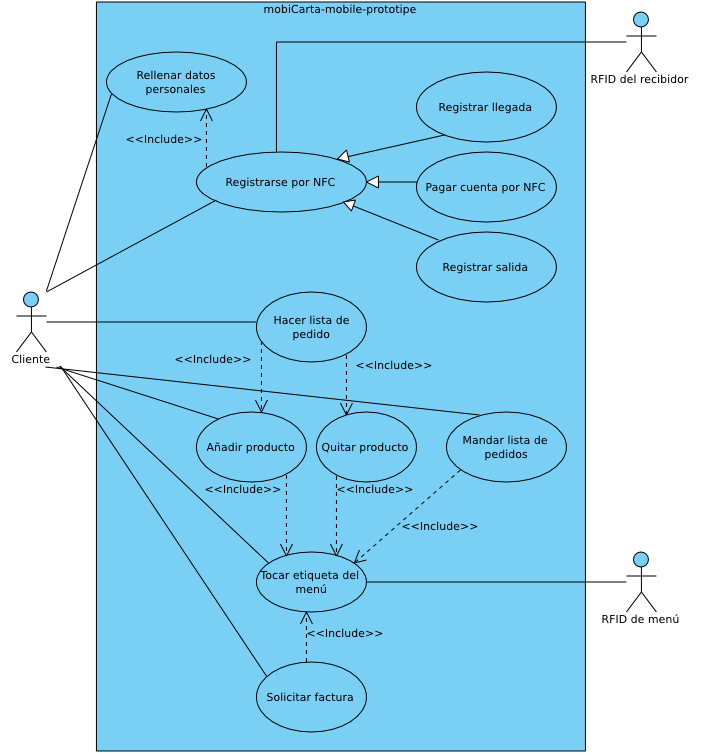
\includegraphics[width=1\textwidth]{ucdM-phase3.png}
      \caption{Diagrama de casos de uso del primer prototipo de la aplicación
      móvil.}
      \label{fig:ucdM-phase3}
    \end{center}
  \end{figure}

Los principales casos de uso se explican en las secciones
\ref{subsec:mobile-receiver} y \ref{subsec:mobile-bar} donde se encuentran
definidas las comunicaciones \texttt{Bluetooth} entre la aplicación móvil y
la aplicación del recibidor y de la barra.

La funcionalidad de este prototipo se ha implementado a través de la
definición de las siguientes clases:
\begin{itemize}
\item \textbf{\texttt{MobiCarta}}. Es la clase principal del \texttt{MIDlet}. 
Implementa la \acs{GUI} y las funciones que permiten la captura de los eventos 
\acs{NFC}.
\item \textbf{\texttt{ProfileManager}}. Se encarga de generar un perfil de 
cliente con los datos que el usuario ha introducido (a través de un 
formulario); y lo recupera cuando alguna operación lo necesita.
\item \textbf{\texttt{FileIO}}. Implementa la lógica que permite realizar 
lecturas y escrituras en archivos. En este caso, se utiliza para guardar y 
recuperar el perfil de cliente que \texttt{ProfileManager} ha 
generado.
\item \textbf{\texttt{ProductsListManager}}. Mantiene la lista de productos
de un pedido. Esta lista se elabora a partir de las interacciones del
dispositivo móvil con las etiquetas \acs{RFID} de una carta de productos.
\item \textbf{\texttt{Client}}. Almacena los datos personales de un cliente
(DNI, nombre, appellidos y dirección).
\item \textbf{\texttt{Address}}. Define la dirección del domicilio del cliente
(calle, número, código postal, localidad y provincia).
\item \textbf{\texttt{Order}}. Contiene la información de un pedido. Esto
es, el nombre y la cantidad de un tipo determinado de producto.
\end{itemize}

La figura \ref{fig:cdM-phase3} muestra el \textbf{diagrama de clases} del
prototipo de la aplicación móvil en esta fase:

  \begin{figure}[H]
    \begin{center}
      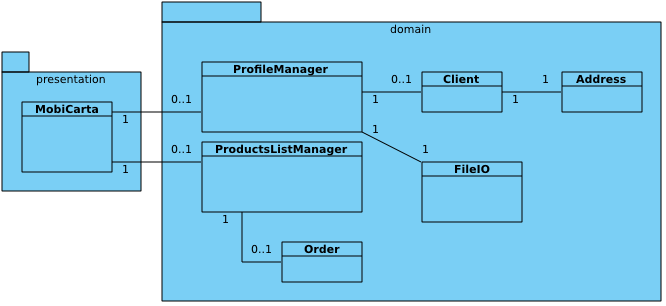
\includegraphics[width=0.9\textwidth]{cdM-phase3.png}
      \caption{Diagrama de clases del prototipo de la aplicación móvil
      (Fase 4).}
      \label{fig:cdM-phase3}
    \end{center}
  \end{figure}

Para implementar la funcionalidad \acs{NFC} se ha hecho uso de la
librería \texttt{\acs{JSR}-257} siguiendo los procedimientos descritos en el 
Anexo \ref{chap:jsr257}.

Los tipos de etiqueta reconocibles por la aplicación están definidos en el 
anexo \ref{chap:tags}.

\subsection{Comunicación \texttt{Bluetooth} entre móvil y \emph{recibidor}}
\label{subsec:mobile-receiver}
La comunicación \texttt{Bluetooth} entre el dispositivo móvil y la aplicación
del \emph{recibidor} posibilitará la autentificación del cliente \acs{NFC}
ante el sistema.

\subsubsection{Análisis de requisitos}
Los requisitos que deben cumplir las comunicaciones \texttt{Bluetooth} entre
los dispositivos móviles y la aplicación del \emph{recibidor} son los
siguientes:
\begin{enumerate}
\item La aplicación del dispositivo móvil será la que inicie siempre la
comunicación \texttt{Bluetooth}.
\item La comunicación se iniciará cuando el cliente toque con su dispositivo
móvil la etiqueta \acs{RFID} que se encuentra en la zona del \emph{recibidor}.
\item La comunicación consistirá en un mensaje enviado por parte de la
aplicación móvil y la respuesta a este mensaje por parte de la aplicación
del \emph{recibidor}.
\item La aplicación móvil siempre enviará los mismos datos, o lo que es lo
mismo, siempre enviará los datos personales del cliente. Estos datos los
mandará como una cadena codificada con formato \acs{XML}.
\item La respuesta de la aplicación del \emph{recibidor} dependerá del estado
del cliente (\emph{el cliente llega}, \emph{el cliente paga} o \emph{el cliente
se va}). En principio, la respuesta va a consistir en una cadena con un texto
que indique que la operación se ha realizado de forma satisfactoria.
\item A la hora de establecer una conexión, la aplicación móvil no buscará una
dirección \texttt{Bluetooth} física concreta, sino que buscará un servicio que
tenga un identificador concreto conocido por esta.
\end{enumerate}
\newpage
\subsubsection{Diseño e implementación}
Al \textbf{diagrama de casos de uso} de la aplicación del \emph{recibidor}
visto en la primera fase (figura \ref{fig:ucdR-phase1}) se le añaden los
siguientes casos de uso (figura \ref{fig:ucdR-phase4}):

  \begin{figure}[H]
    \begin{center}
      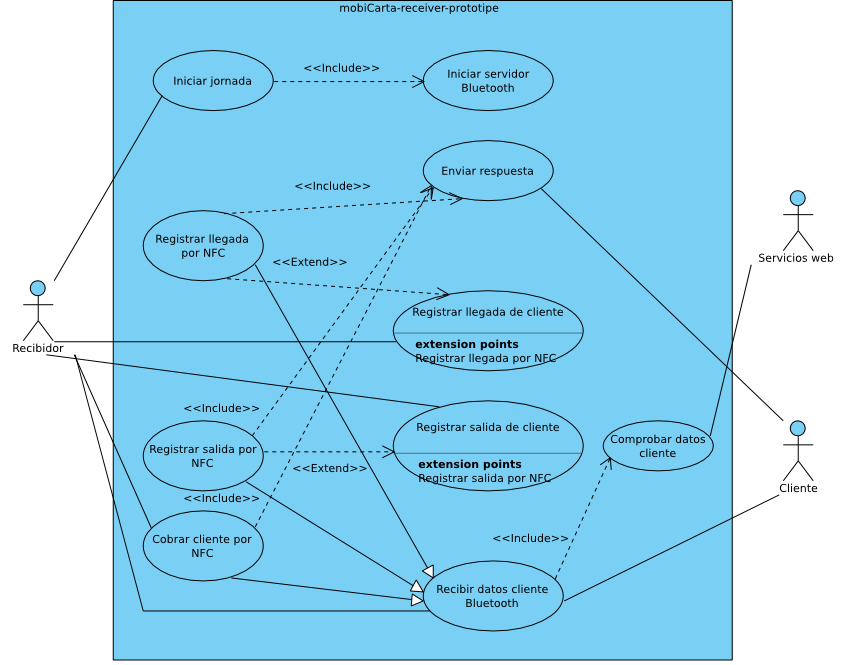
\includegraphics[width=1\textwidth]{ucdR-phase4.png}
      \caption{Casos de uso añadidos al prototipo de la aplicación
      del \emph{recibidor} en esta iteración.}
      \label{fig:ucdR-phase4}
    \end{center}
  \end{figure}

Cuando se lleva a cabo \emph{iniciar jornada}, la aplicación inicia un
\emph{servidor Bluetooth} que se encarga de ofrecer un servicio a los
\emph{clientes \acs{NFC}}. Este servicio está preparado para recibir
los datos personales de los \emph{clientes \acs{NFC}} que pasan por la
zona del \emph{recibidor}, ya sea para registrar su entrada, su intención de
pagar vía \acs{NFC} o su salida:
\begin{itemize}
\item En el caso uso \emph{registrar salida por \acs{NFC}}, cuando el 
servidor \texttt{Bluetooth} recibe los datos de un usuario (en formato
\acs{XML}), los envía al \emph{servicio web} correspondiente, para que este le 
informe del estado del cliente (\emph{cliente que llega}, \emph{cliente que 
paga} o \emph{cliente que se va}). En este caso como es \emph{cliente que se 
va}, la aplicación del \emph{recibidor} muestra un mensaje emergente informando 
del cliente que se va. Por su parte, el servidor \texttt{Bluetooth} manda al 
cliente un mensaje de confirmación, del tipo \emph{gracias por su visita}. El 
\emph{maître}, encargado de manejar la aplicación del \emph{recibidor}, debe 
confirmar finalmente que el cliente se ha ido. Al hacerlo, informa a la 
aplicación web que el cliente ha abandonado su mesa y este le devuelve la nueva 
situación del restaurante. La figura \ref{fig:sdR-phase4} (página
\pageref{fig:sdR-phase4}) muestra el \textbf{diagrama de secuencia} del caso de 
uso \emph{registrar salida por \acs{NFC}}.

\item El caso de \textbf{registrar llegada por \acs{NFC}}, es muy parecido al
anterior, salvo que el mensaje enviado al cliente es de bienvenida.
\item Por su parte, el caso de uso \textbf{cobrar cliente por \acs{NFC}} tiene
la peculiaridad de que ocurre cuando un cliente \acs{NFC} va a registrar su
salida, pero aún no ha pagado su cuenta. Al recibir los datos del cliente y
consultar con el servicio web que su estado es el descrito anteriormente, el
\emph{recibidor} vuelve a mandar otra petición a la aplicación de los servicios
web, esta vez de facturación. Con los datos del cliente y los datos de la
factura se realiza el cargo del importe, se le envía al cliente el resumen de
la operación y, de paso, se desocupa su mesa, para que este no tenga que
realizar la interacción de \emph{registrar salida por \acs{NFC}}. La figura
\ref{fig:sdR2-phase4} (página \pageref{fig:sdR2-phase4}) muestra el
\textbf{diagrama de secuencia} de este caso de uso.
\end{itemize}

  \begin{sidewaysfigure}[hp]
    \begin{center}
      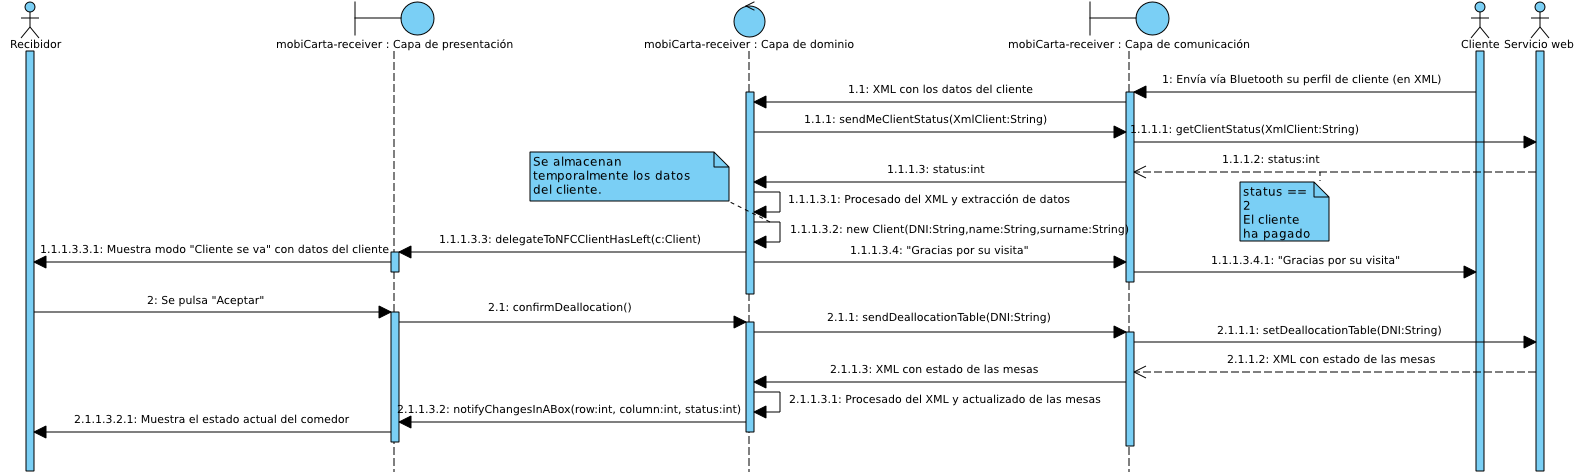
\includegraphics[width=1\textwidth]{sdR-phase4.png}
      \caption{Diagrama de secuencia del caso de uso \emph{registrar salida
      por \acs{NFC}}.}
      \label{fig:sdR-phase4}
    \end{center}
  \end{sidewaysfigure}

  \begin{sidewaysfigure}[hp]
    \begin{center}
      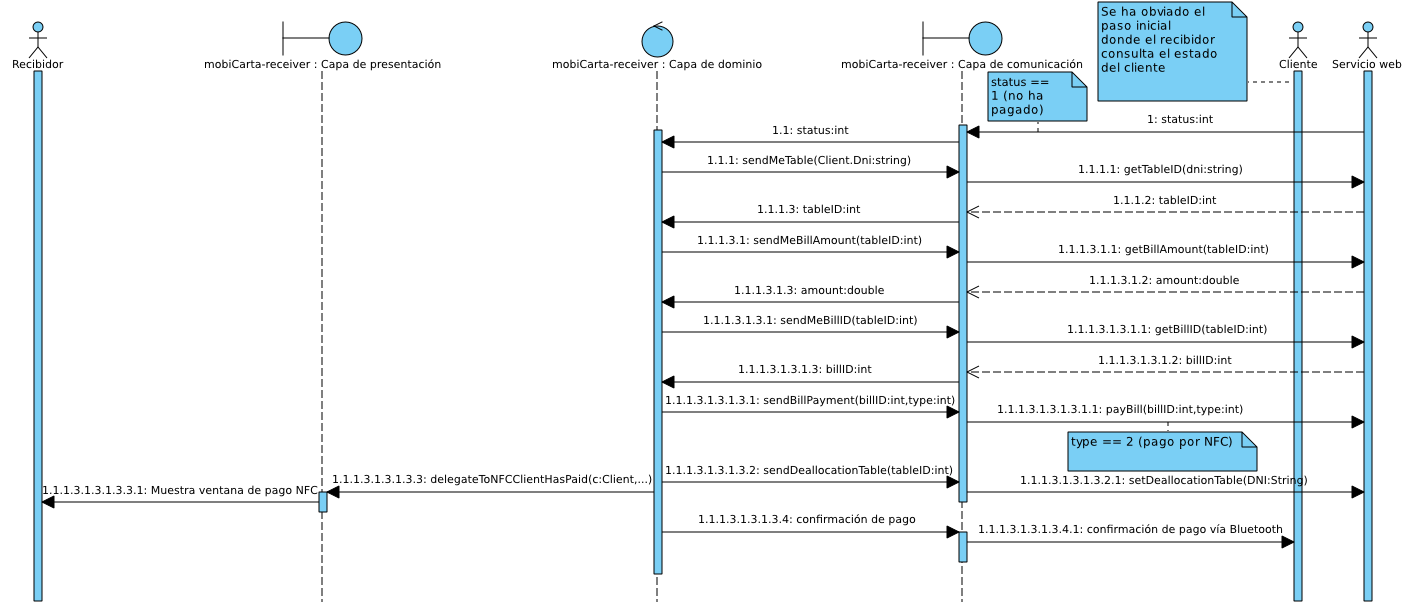
\includegraphics[width=1\textwidth]{sdR2-phase4.png}
      \caption{Diagrama de secuencia del caso de uso \emph{cobrar cliente
      por \acs{NFC}}.}
      \label{fig:sdR2-phase4}
    \end{center}
  \end{sidewaysfigure}

Por otro lado, al \textbf{diagrama de casos de uso} del primer prototipo
de la aplicación móvil (figura \ref{fig:ucdM-phase3}, página
\pageref{fig:ucdM-phase3}) se le añaden los siguientes caso de uso (figura
\ref{fig:ucdM-phase4}):

  \begin{figure}[H]
    \begin{center}
      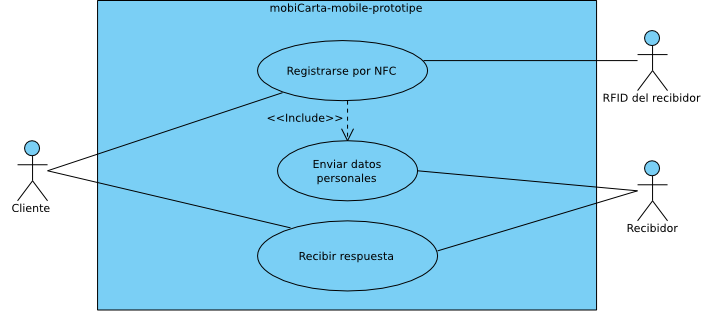
\includegraphics[width=0.9\textwidth]{ucdM-phase4.png}
      \caption{Casos de uso añadidos al prototipo de la aplicación
      móvil en esta iteración.}
      \label{fig:ucdM-phase4}
    \end{center}
  \end{figure}

Los casos de uso \textbf{registrar llegada}, \textbf{pagar cuenta por
\acs{NFC}} y \textbf{registrar salida}, que forman parte de la generalización
de \textbf{Registrarse por \acs{NFC}}, son llevados a cabo por parte del
cliente de forma casi idéntica, ya que el que determina el caso de uso que
se está realizando es la aplicación del \emph{recibidor}. La figura
\ref{fig:sdM-phase4} (página \pageref{fig:sdM-phase4}) muestra el
\textbf{diagrama de secuencia} del caso de uso \emph{registrar entrada}.

  \begin{sidewaysfigure}[hp]
    \begin{center}
      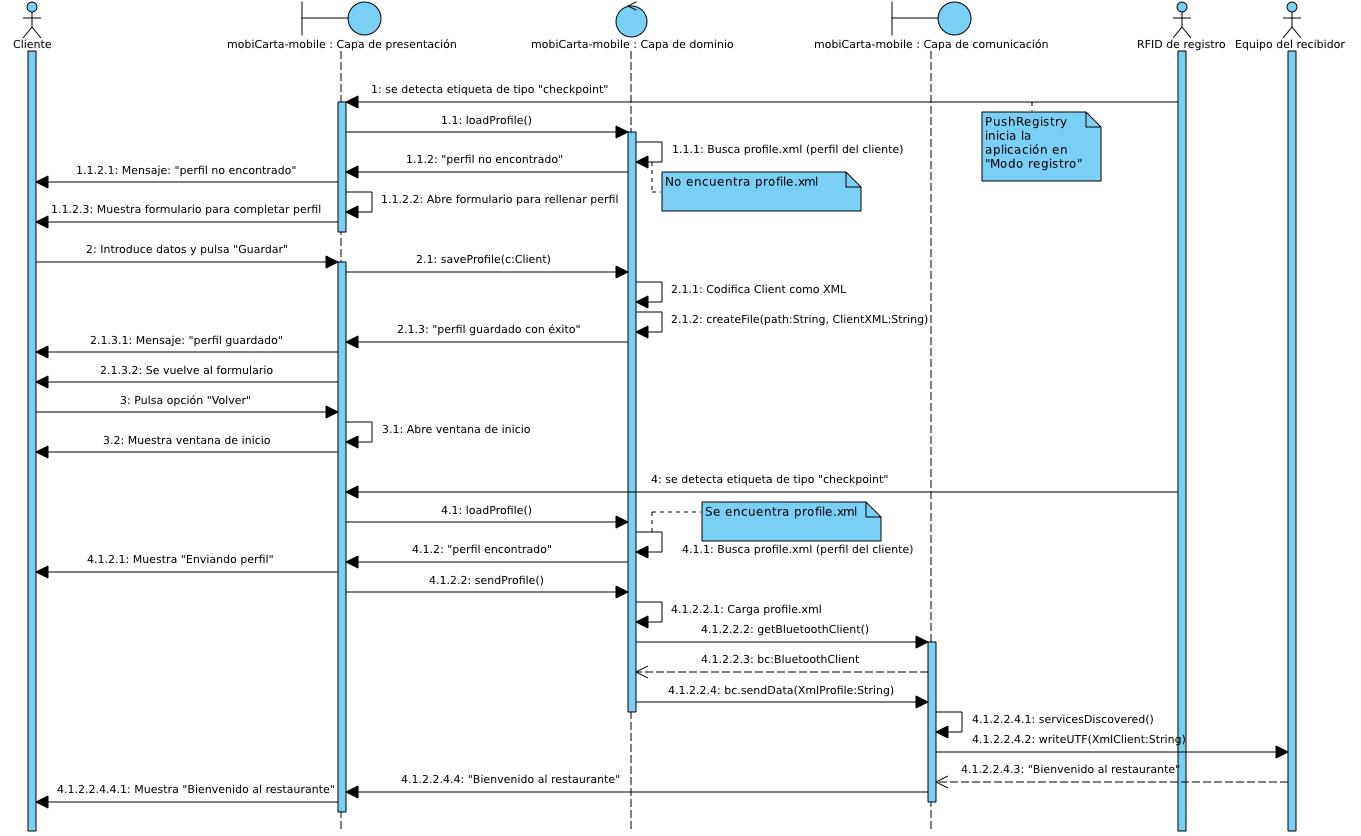
\includegraphics[width=1\textwidth]{sdM-phase4.png}
      \caption{Diagrama de secuencia del caso de uso \emph{registrar entrada},
      de la aplicación móvil.}
      \label{fig:sdM-phase4}
    \end{center}
  \end{sidewaysfigure}
\newpage
Cuando el móvil se acerca a una etiqueta de tipo \emph{checkpoint}, se
arranca automáticamente la aplicación móvil en \emph{modo registro}. Lo
primero que se comprueba es que existe un archivo llamado \emph{profile.xml},
que guarda la información de usuario del cliente. En caso de no encontrarlo,
la aplicación insta al cliente a que rellene un formulario con sus datos.
Una vez completados, el usuario pulsa la opción \emph{Guardar} y la
aplicación se encarga de codificar la información en formato \acs{XML} y de
guardarla en \emph{profile.xml}. Para volver a intentar registrarse en el
sistema, el cliente deberá aproximar de nuevo su móvil a la etiqueta
\emph{checkpoint}. Esta vez, la aplicación encontrará el archivo
\emph{profile.xml}, cargará su información y buscará el servicio
\texttt{Bluetooth} que ofrece la aplicación del \emph{recibidor} para
registrar clientes. Cuando lo encuentre, le mandará la cadena con los datos
del cliente. Finalmente, la aplicación del \emph{recibidor} confirmará que
le ha llegado la información del cliente y que por tanto ha quedado
registrada, en este caso, la entrada al restaurante.

En cuanto al diseño de clases de los prototipos:
\begin{itemize}
\item El \textbf{prototipo del recibidor} añade la clase
\textbf{\texttt{BluetoothServer}}. Esta clase implementa un servidor
\texttt{Bluetooth} que publica un servicio de registro de clientes. Este
servidor ha sido implementado utilizando la biblioteca \acs{DLL}
\texttt{32feet} (siguiendo los pasos descritos en el Anexo \ref{chap:32feet}).
\item El \textbf{prototipo del móvil} por su parte, añade la clase
\textbf{\texttt{BluetoothClient}}. Esta clase implementa un cliente
\texttt{Bluetooth} que se encarga de buscar el servicio \texttt{Bluetooth}
publicado por el \emph{recibidor} y de enviarle el perfil de cliente del
usuario. Dependiendo del estado en el que se encuentre el cliente, recibirá
una respuesta distinta por parte del \emph{recibidor}. El cliente
\texttt{Bluetooth} ha sido implementado haciendo uso de la librería
\texttt{\acs{JSR}-82} (utilizando las operaciones definidas en el Anexo
\ref{chap:jsr82}).
\end{itemize}
\newpage
\subsection{Comunicación \texttt{Bluetooth} entre móvil y \emph{barra}}
\label{subsec:mobile-bar}
La comunicación \texttt{Bluetooth} entre el dispositivo móvil y la aplicación
de la \emph{barra} permitirá al cliente \acs{NFC} realizar pedidos y conocer
cuál es el importe de la cuenta, sin necesidad de avisar a ningún camarero.

\subsubsection{Análisis de requisitos}
Los requisitos que deben cumplir las comunicaciones \texttt{Bluetooth} entre
los dispositivos móviles y la aplicación de la \emph{barra} son los
siguientes:
\begin{enumerate}
\item La aplicación del dispositivo móvil será la que inicie siempre la
comunicación \texttt{Bluetooth}.
\item La comunicación se iniciará cuando el cliente confirme (a través de la
etiqueta correspondiente) que va a realizar un pedido con los productos que ha 
ido seleccionando de la carta de etiquetas \acs{RFID}. También puede iniciar
una comunicación para solicitar la cuenta de lo que ha consumido.
\item Todas las comunicaciones consistirán en un mensaje enviado por parte de
la aplicación móvil y la respuesta a este por parte de la aplicación de la
\emph{barra}.
\item La aplicación móvil enviará un mensaje con el identificador del cliente
y los productos (y la cantidad de cada uno de ellos) que forman parte del
pedido o, en caso de solicitar la cuenta, simplemente el identificador del
cliente y el concepto \emph{facturar mesa}. Estos datos los mandará como una
cadena codificada con formato \acs{XML}.
\item La respuesta de la aplicación de la \emph{barra} consistirá en una cadena 
con un texto que indique si la operación se ha completado o no 
satisfactoriamente.
Para la respuesta ante una solicitud de facturación, la aplicación calculará
el importe total de lo que debe la mesa y enviará un resumen (codificado
en formato \acs{XML}) con los productos consumidos y la cantidad a abonar.
\item A la hora de establecer una conexión, la aplicación móvil no buscará una
dirección \texttt{Bluetooth} física concreta, sino que buscará un servicio que
tenga un identificador concreto conocido por esta (distinto al servicio
ofrecido por la aplicación del \emph{recibidor}).
\end{enumerate}

\subsubsection{Diseño e implementación}
El \textbf{diagrama de casos de uso} del prototipo de la aplicación de la
\emph{barra} va a ser complementado con los siguientes casos de uso (figura
\ref{fig:ucdB-phase5}):

  \begin{figure}[H]
    \begin{center}
      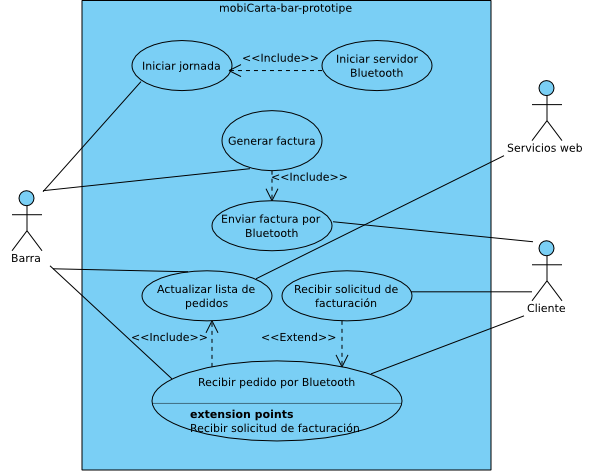
\includegraphics[width=0.8\textwidth]{ucdB-phase5.png}
      \caption{Casos de uso añadidos al prototipo de la aplicación
      de la \emph{barra} en esta iteración.}
      \label{fig:ucdB-phase5}
    \end{center}
  \end{figure}

Por su parte, el \textbf{diagrama de casos de uso} de la aplicación móvil
añade los siguientes casos de uso (figura \ref{fig:ucdM-phase5}):

  \begin{figure}[H]
    \begin{center}
      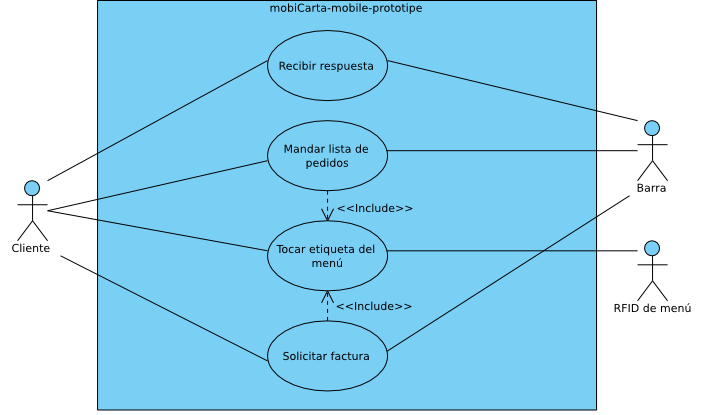
\includegraphics[width=0.9\textwidth]{ucdM-phase5.png}
      \caption{Casos de uso añadidos al prototipo de la aplicación
      móvil en esta iteración.}
      \label{fig:ucdM-phase5}
    \end{center}
  \end{figure}

En este caso se incorporan dos importantes casos de uso:
\begin{itemize}
\item \textbf{Mandar lista de pedidos}. Para solicitar un pedido, antes hay
que elaborar una lista con los productos que el cliente desea. El prototipo
inicial de la aplicación móvil ya permitía realizar la lista de productos
pero no permitía enviarla. La figura \ref{fig:sdM1-phase5} (página
\pageref{fig:sdM1-phase5}) muestra el \textbf{diagrama de secuencia} de este
caso de uso.

Cuando el dispositivo móvil contacta con una etiqueta de tipo \emph{product},
la aplicación móvil arranca automáticamente en \emph{modo pedido}. Todas las
etiquetas de tipo \emph{product} contienen el nombre del producto al que
representan. Este nombre aparecerá como el primer elemento de la lista de
productos para el pedido. Cuando el móvil contacta con una segunda etiqueta
\emph{product}, la aplicación comprueba la lista de productos existente; si
el producto ya aparece en la lista, incrementa el número de productos de ese
tipo; si no, el producto se añade a la lista en una nueva línea.

Para enviar el pedido, el usuario debe acercar su móvil a una etiqueta de
tipo \emph{send-order}. En ese momento, la aplicación buscará el archivo
\emph{profile.xml} para extraer la información del usuario y compondrá un
\acs{XML} con estos datos y con la lista de productos elaborada. Por último,
la aplicación buscará el servicio \texttt{Bluetooth} ofrecido por la aplicación
de la \emph{barra} y le mandará una cadena con el \acs{XML}. La aplicación
de la \emph{barra} contestará si ha recibido la cadena correctamente.

\item \textbf{Solicitar factura}. El usuario dispone de la opción de conocer,
a través de la aplicación móvil, cuál es el importe que debe abonar por los
pedidos realizados. La figura \ref{fig:sdM2-phase5} (página
\pageref{fig:sdM2-phase5}) muestra el \textbf{diagrama de secuencia} de los
pasos que debe seguir.

Cuando el dispositivo móvil detecta la presencia de una etiqueta de tipo
\emph{bill-request}, arranca automáticamente la aplicación en \emph{modo
solicitar facturación}. A continuación, la aplicación busca el archivo
\emph{profile.xml} para extraer la información del usuario y con ello componer
un \acs{XML} con el motivo \emph{solicitar facturación}. Este \acs{XML} se
manda al servicio correspondiente de la aplicación de la \emph{barra}. Y,
finalmente, esta responde con un resumen (en \acs{XML}) de la factura de la 
mesa que ocupa el cliente. Este resumen contiene información como: cliente, 
mesa, número de factura, pedidos realizados, subtotal, descuentos, IVA e
importe total.
\end{itemize}

  \begin{sidewaysfigure}[hp]
    \begin{center}
      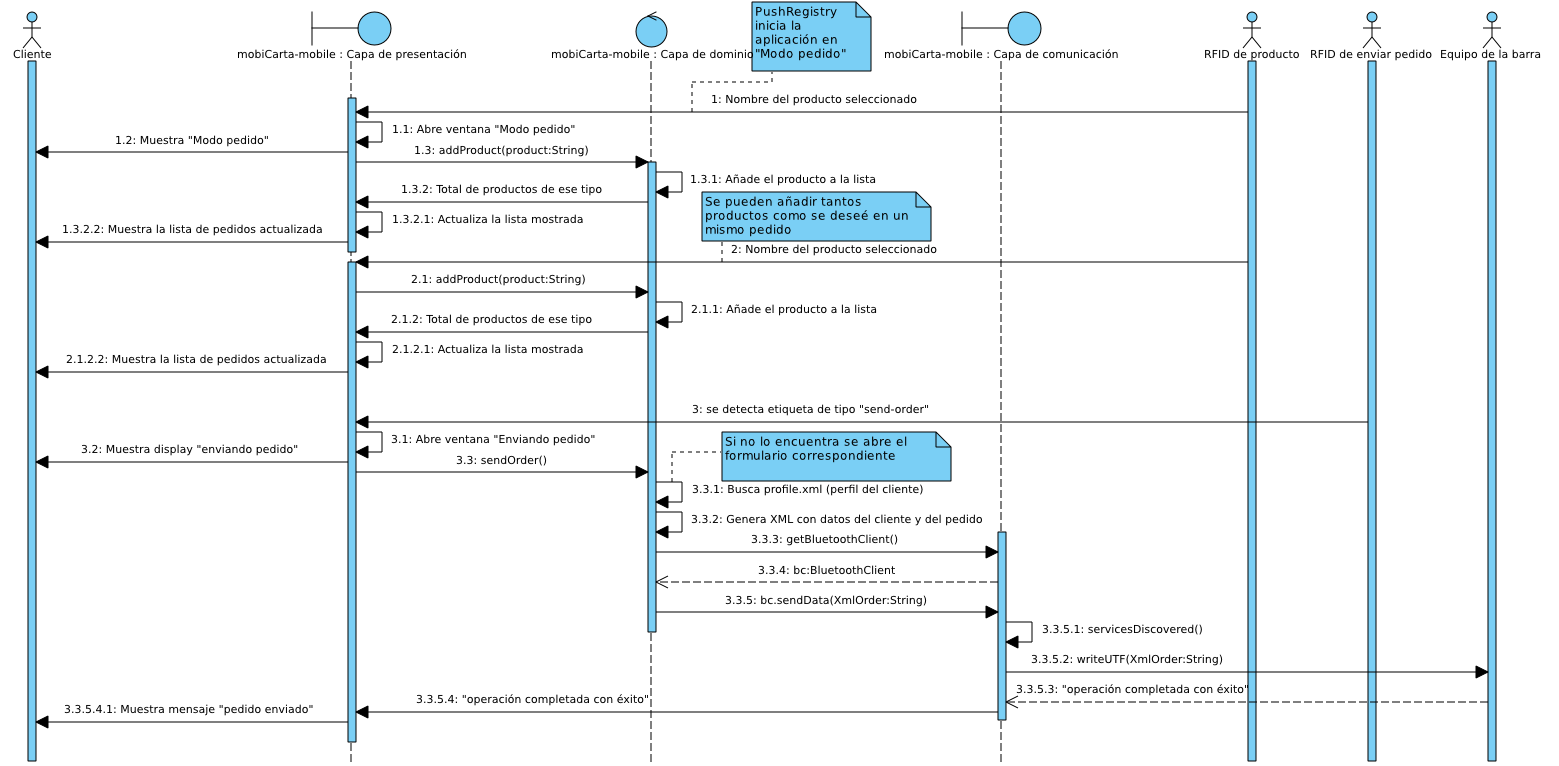
\includegraphics[width=1\textwidth]{sdM1-phase5.png}
      \caption{Diagrama de secuencia del caso de uso \emph{mandar lista
      de pedidos}. En este caso el cliente solicita dos productos.}
      \label{fig:sdM1-phase5}
    \end{center}
  \end{sidewaysfigure}

  \begin{sidewaysfigure}[hp]
    \begin{center}
      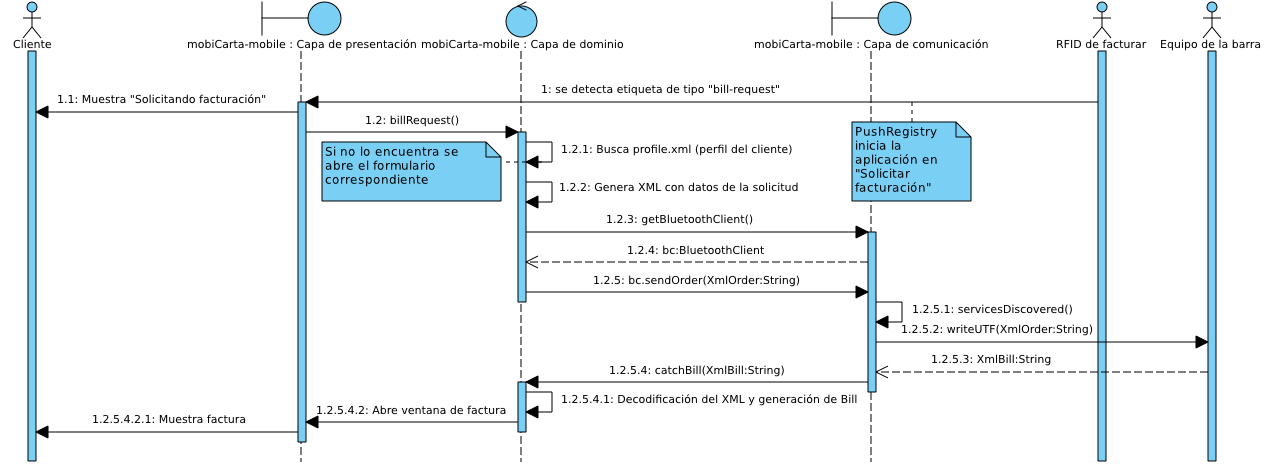
\includegraphics[width=1\textwidth]{sdM2-phase5.png}
      \caption{Diagrama de secuencia del caso de uso \emph{solicitar factura}.}
      \label{fig:sdM2-phase5}
    \end{center}
  \end{sidewaysfigure}
\newpage
En cuanto al diseño de clases de los prototipos:
\begin{itemize}
\item El \textbf{prototipo de la barra} añade las siguientes clases:
  \begin{itemize}
  \item \textbf{\texttt{BluetoothServer}}. Esta clase es similar a su homónima 
  en el prototipo del recibidor. Sin embargo, en este caso, publica un servicio 
  que recoge los pedidos de los clientes \acs{NFC} y las solicitudes de
  facturación.
  \item \textbf{\texttt{ShortBill}}. Almacena la información resumida de una 
  factura. Cuando un cliente \acs{NFC} solicita una factura a través de una 
  petición por \texttt{Bluetooth}, la \emph{aplicación de la barra} no le manda 
  una factura detallada (tipo \texttt{Bill}), sino que le envía una factura más
  simplificada con: el nombre de restaurante, la fecha, los pedidos realizados
  y el importe total.
  \end{itemize}
\item El \textbf{prototipo del móvil} por su parte, añade las siguientes
clases:
  \begin{itemize}
  \item La clase \textbf{\texttt{BluetoothClient}} adapta su funcionalidad para 
  poder comunicarse con el servicio publicado por la \emph{aplicación de la 
  barra}.
  \item \textbf{\texttt{BillManager}}. Se encarga de decodificar la información 
  de recibida tras una solicitud de facturación. Con esta información crea un
  objeto de tipo \textbf{\texttt{Bill}}. La información de cada uno de los
  productos que aparecen en la factura está contenida en un objeto de tipo
  \textbf{\texttt{BillItem}} (producto, cantidad, precio por unidad, descuentos
  y precio total).
  \end{itemize}
\end{itemize}
\newpage
\subsection{Módulo recomendador}
El objetivo del módulo recomendador es ofrecer al cliente una serie de
servicios extra que le incentiven a seguir utilizando la tecnología \acs{NFC}
dentro de dicho establecimiento. Implementar el módulo recomendador implicará
realizar cambios en el prototipo de los servicios web y la base de datos, en
el prototipo del \emph{recibidor} y en el prototipo de la aplicación móvil.
Al término de esta iteración se habrá obtenido la primera versión del prototipo
final del sistema.

\subsubsection{Análisis de requisitos}
Los requisitos que debe satisfacer el módulo recomendador son los siguientes:
\begin{enumerate}
\item Debe ofrecer la siguiente información al cliente:
  \begin{itemize}
  \item Cuáles son los platos que más ha consumido.
  \item Qué productos de la carta tienen algún descuento.
  \item Teniendo en cuenta los productos favoritos del cliente, qué productos
  similares a estos pueden gustarle.
  \end{itemize}
\item Será ejecutado por la aplicación de los servicios web.
\item La base de datos contará con una nueva tabla (\emph{historial}) con el
histórico de pedidos que ha realizado el cliente a lo largo de sus visitas
al restaurante. Esta tabla se utilizará para calcular las recomendaciones para
un cliente.
\item El cliente recibirá las recomendaciones cuando registre su entrada en el
restaurante (vía \texttt{Bluetooth}), aunque también podrá consultarlas mientras
está elaborando una lista para un pedido.
\end{enumerate}

\subsubsection{Diseño e implementación}
El diseño del módulo recomendador va a afectar a los servicios web, al 
prototipo del \emph{recibidor} y al prototipo de la aplicación móvil.

La aplicación de los servicios web va a añadir el caso de uso \emph{calcular 
recomendaciones} (figura \ref{fig:ucdW-phase6}):

  \begin{figure}[H]
    \begin{center}
      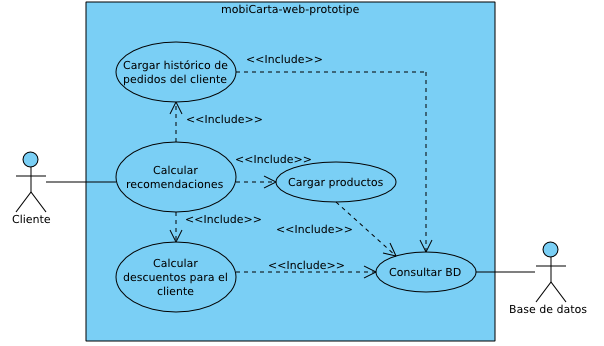
\includegraphics[width=0.8\textwidth]{ucdW-phase6.png}
      \caption{Caso de uso \emph{calcular recomendaciones} añadido al prototipo
      final de los servicios web.}
      \label{fig:ucdW-phase6}
    \end{center}
  \end{figure}

Cuando el servicio web recibe una petición de \emph{calcular recomendaciones} 
para un cliente, en primer lugar, accede a la base de datos en busca de la
información de dicho cliente. Esta información la va a utilizar para conocer
si dispone o no de algún descuento por número de visitas realizadas. En
segundo lugar, se accede de nuevo a la base de datos en busca del historial
de pedidos del cliente y de la lista de productos visibles (es decir, los están
a la venta). Estos dos parámetros van a servir para calcular hasta tres tipos
distintos de recomendaciones:
\begin{enumerate}
\item Una lista de los productos que el cliente ha consumido más habitualmente. 
Ya que es muy probable que los vuelva a consumir.
\item Una lista con los productos que están en promoción. Esto es, productos 
cuya segunda, tercera, \dots unidad tiene un descuento de un tanto por ciento.
\item Y una lista de los productos similares a los más habitualmente 
consumidos. Es muy probable que si a un cliente le gusta un tipo de plato, le 
gusten también platos similares a este.
\end{enumerate}
Por último, se codifican en \acs{XML} los resultados obtenidos y se le
devuelven al cliente del servicio web. La figura \ref{fig:ucdW-phase6}
(página \pageref{fig:ucdW-phase6}) muestra el \textbf{diagrama de secuencia}
de este caso de uso.

  \begin{sidewaysfigure}[hp]
    \begin{center}
      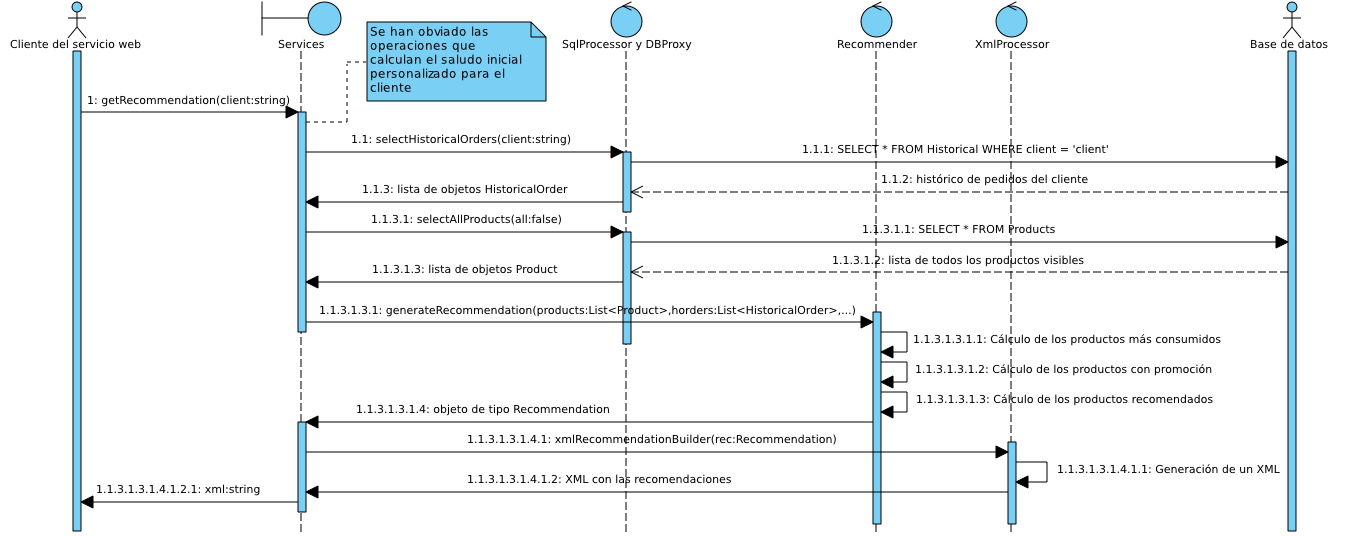
\includegraphics[width=0.8\textwidth]{sdW-phase6.png}
      \caption{Diagrama de secuencia del caso de uso \emph{calcular 
      recomendaciones}.}
      \label{fig:sdW-phase6}
    \end{center}
  \end{sidewaysfigure}
\newpage
A continuación, se va a profundizar en cómo se realiza el proceso de cálculo
de recomendaciones (ver figura \ref{fig:recommender}):

  \begin{figure}[H]
    \begin{center}
      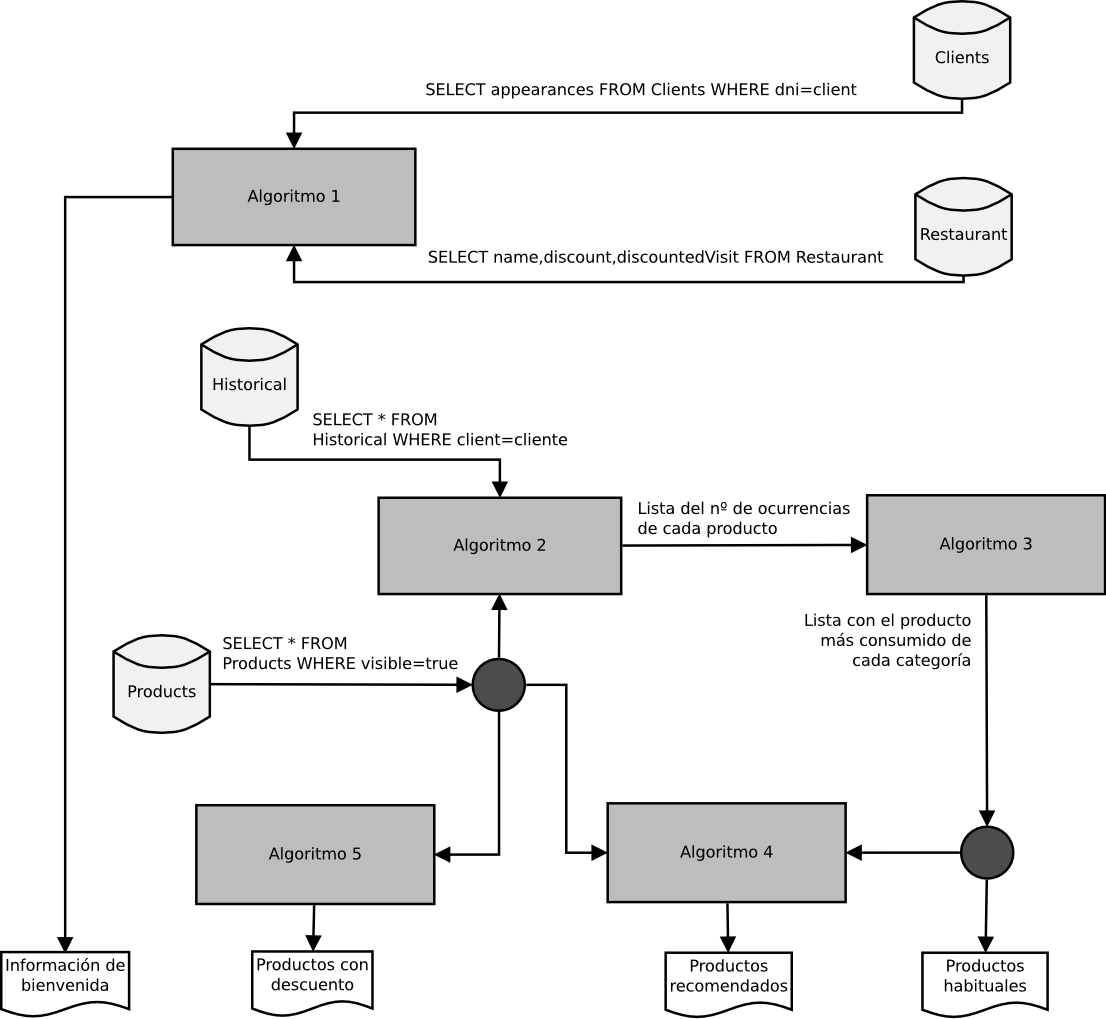
\includegraphics[width=0.8\textwidth]{recommender.png}
      \caption{Cálculo de las recomendaciones para el cliente
      ``\emph{client}''.}
      \label{fig:recommender}
    \end{center}
  \end{figure}

El recomendador hace uso de cinco algoritmos:
\begin{itemize}
\item \textbf{\emph{Algoritmo 1}}.
  \begin{itemize}
  \item \emph{Entradas:}
    \begin{itemize}
    \item De la tabla \texttt{Clients}, se selecciona el número de apariciones 
    del cliente cuyo DNI corresponde con el del cliente destinatario de la
    recomendación.
    \item De la tabla \texttt{Restaurant}, se selecciona el nombre, el
    porcentaje de descuento y el número de visitas a realizar para aplicar un
    descuento.
    \end{itemize}
  \item \emph{Procedimiento:} si el porcentaje de descuentos es distinto de 0,
  se comprueba si el número de visitas realizadas por el cliente es múltiplo 
  del número de visitas a realizar para recibir un descuento. Si es así,
  se crea un mensaje que lo indique. En caso contrario, se generará un
  mensaje informando del número de visitas que el cliente ha de realizar para 
  recibir el próximo descuento.
  \item \emph{Salida:} se genera un mensaje de bienvenida del restaurante
  ``\emph{tal}'' y se informa de los descuentos calculados por el algoritmo.
  \end{itemize}
\item \textbf{\emph{Algoritmo 2}}.
  \begin{itemize}
  \item \emph{Entradas:}
    \begin{itemize}
    \item De la tabla \texttt{Historical}, se extrae el historial de pedidos
    del cliente.
    \item De la tabla \texttt{Products}, se seleccionan todos los productos
    que están a la venta durante la jornada actual.
    \end{itemize}
  \item \emph{Procedimiento:} del historial de pedidos, se eliminan aquellos
  cuyos productos que no estén a la venta. Con los restantes, se calcula en
  número de veces que se ha consumido cada tipo de producto.
  \item \emph{Salida:} al final se obtiene una lista con los productos
  consumidos (y a la venta) que ha consumido el cliente y con el número de
  veces que ha consumido cada uno de esos productos.
  \end{itemize}
\item \textbf{\emph{Algoritmo 3}}.
  \begin{itemize}
  \item \emph{Entrada:} la salida del \emph{Algoritmo 3}.
  \item \emph{Procedimiento:} se clasifican productos obtenidos por
  el \emph{Algoritmo 3} por categorías de productos y se cogen los productos
  más consumidos de cada categoría.
  \item \emph{Salida:} se obtiene una lista con el producto más consumido de
  cada categoría.
  \end{itemize}
\item \textbf{\emph{Algoritmo 4}}.
  \begin{itemize}
  \item \emph{Entradas:}
    \begin{itemize}
    \item Se coge el resultado obtenido por el \emph{Algoritmo 3}.
    \item Y de la tabla \texttt{Products}, se seleccionan los productos que 
    están a la venta.
    \end{itemize}
  \item \emph{Procedimiento:} se coge cada uno de los productos de la lista
  generada por el \emph{Algoritmo 3} y se calcula su similitud con cada uno
  de los productos de su misma categoría. La similitud entre dos productos se 
  obtiene calculando el número de palabras clave que tienen en común. Estas 
  palabras clave están contenidas en la descripción de cada producto. El 
  producto con más palabras en común con el producto de referencia, formará 
  parte de la lista de productos recomendados.
  \item \emph{Salida:} se obtiene una lista con el producto más similar al
  obtenido por el \emph{Algoritmo 3}, de cada categoría de productos.
  \end{itemize}
\item \textbf{\emph{Algoritmo 5}}.
  \begin{itemize}
  \item \emph{Entradas:} de la tabla \texttt{Products} se seleccionan los
  productos que tienen descuento.
  \item \emph{Procedimiento:} de todos los productos, se eligen aquellos cuyo
  descuento sea mayor que 0\% y cuyo número de productos a consumir para el
  descuento sea también mayor de 0 unidades.
  \item \emph{Salida:} se obtiene una lista con los productos a la venta que
  tienen algún tipo de descuento.
  \end{itemize}
\end{itemize}

Finalmente, tras el uso de estos cinco algoritmo, el recomendador devuelve 
cuatro resultados:
\begin{enumerate}
\item Una cadena con \textbf{información de bienvenida} personalizada para
el cliente. Esta información será del tipo: ``\emph{Bienvenido al restaurante
\texttt{nombre\_del\_restaurante}. Es su visita número \texttt{numero\_de
\_visita}. La factura de la visita \texttt{visita\_con\_descuento} dispondrá 
de un descuento del \texttt{descuento\_factura} \%}''.
\item Una lista de los \textbf{productos con descuento}.
\item Una lista con los \textbf{productos consumidos más habitualmente}.
\item Una lista de los \textbf{productos recomendados} por su similitud con
los productos más consumidos.
\end{enumerate}

%%%%% Hay que hacerlo.......
%El Anexo \ref{chap:recommender} muestra un ejemplo de cómo funciona el
%módulo recomendador.

Por otra parte, al prototipo de la aplicación del \emph{recibidor} añade un 
único caso de uso (figura \ref{fig:ucdR-phase6}):

  \begin{figure}[H]
    \begin{center}
      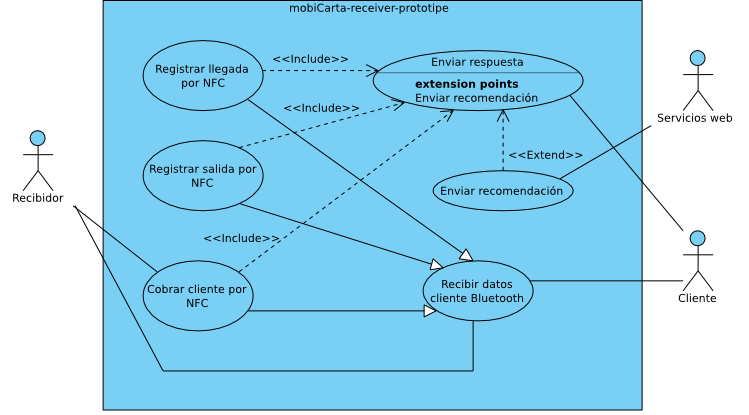
\includegraphics[width=0.8\textwidth]{ucdR-phase6.png}
      \caption{Casos de uso \emph{enviar recomendación} añadido a la aplicación 
      del \emph{recibidor}.}
      \label{fig:ucdR-phase6}
    \end{center}
  \end{figure}

Para implementar la funcionalidad de este caso de uso simplemente, al gestor de 
clientes \texttt{ClientManager}, se le añade una llamada (a través de
\texttt{AdapterWebServices}) que devuelva la recomendación para el cliente
que está solicitando su registro para entrar al restaurante.

Finalmente, al prototipo de la aplicación móvil, se añaden dos nuevos casos de 
uso (figura \ref{fig:ucdM-phase6}):

  \begin{figure}[H]
    \begin{center}
      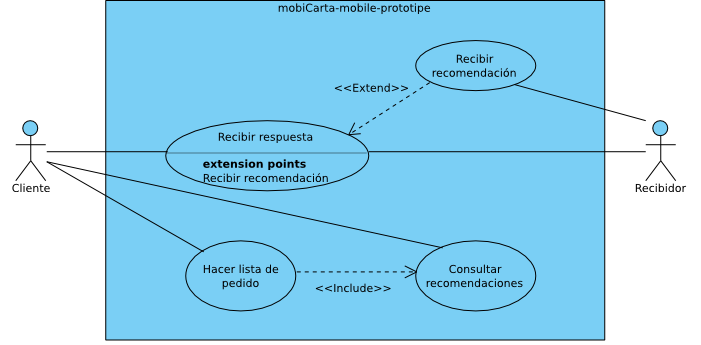
\includegraphics[width=1\textwidth]{ucdM-phase6.png}
      \caption{Se añaden los casos de uso \emph{recibir recomendación} y
      \emph{consultar recomendaciones}.}
      \label{fig:ucdM-phase6}
    \end{center}
  \end{figure}

\begin{itemize}

\item \textbf{Recibir recomendación}. Cuando un cliente \acs{NFC} envía los
datos para registrar su entrada en el restaurante, ya no recibe simplemente
un mensaje de bienvenida (como ocurría en el diagrama de secuencia de la
figura \ref{fig:sdM-phase4}, página \pageref{fig:sdM-phase4}), sino que
recibe una cadena estructurada en \acs{XML} con las recomendaciones calculadas
para dicho cliente. Dicha cadena está formada por un saludo personalizado
de bienvenida, que se mostrará en ese momento en pantalla; y por una lista
de productos recomendados, que se mostrarán cuando se esté elaborando la lista 
de productos para un pedido. El \acs{XML} será almacenado como un archivo en la 
memoria del dispositivo móvil para ser recuperado cuando haga falta.
La figura \ref{fig:sdM-phase6} (página \pageref{fig:sdM-phase6}) muestra el 
\textbf{diagrama de secuencia} de este caso de uso.

\item \textbf{Consultar recomendación}. Cuando un cliente \acs{NFC} está
elaborando la lista de productos de un pedido, tiene la opción de consultar
las recomendaciones que la \emph{aplicación del recibidor} le envió cuando
llegó al restaurante. Estas recomendaciones son cargadas del archivo que se
creó en el caso de uso anterior y están divididas en tres categorías:
\emph{productos más consumidos}, \emph{productos con descuento} y
\emph{productos recomendados}.
\end{itemize}

  \begin{sidewaysfigure}[hp]
    \begin{center}
      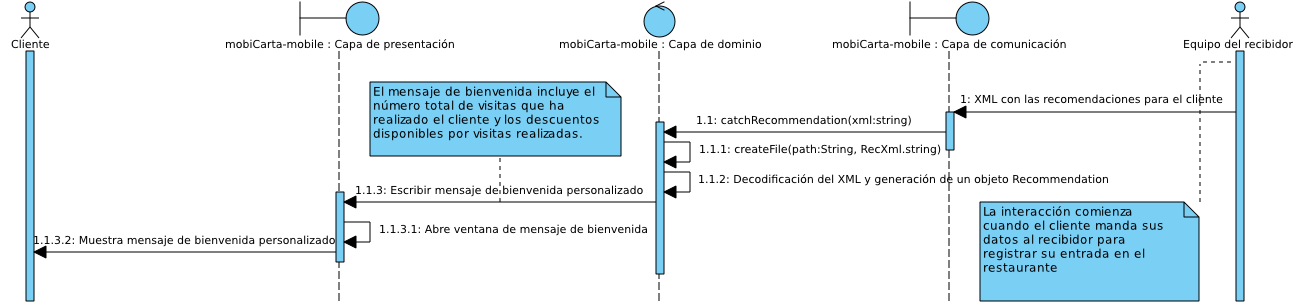
\includegraphics[width=0.8\textwidth]{sdM-phase6.png}
      \caption{Diagrama de secuencia del caso de uso \emph{recibir 
      recomendación}.}
      \label{fig:sdM-phase6}
    \end{center}
  \end{sidewaysfigure}

Terminado el módulo recomendador, se da por finalizado el prototipo completo
del sistema. Los diagramas de clases de los prototipos finales pueden
consultarse en el Anexo \ref{chap:classDiagrams}.

\section{Pruebas}
\label{sec:testing}
Una prueba es una actividad por la cual un sistema o uno de sus componentes
es ejecutado bajo unas circunstancias previamente especificadas. Los resultados
obtenidos son registrados y observados y sirven para evaluar algún aspecto
de dicho sistema o componente.

Como el objetivo final de este proyecto es el de diseñar e implementar el 
\textbf{prototipo de un sistema} que va a ser integrado en un restaurante y que 
va a ser utilizado por sus empleados y clientes, se ha dejado de lado la 
realización de pruebas unitarias, de integración, de sistema y funcionales; 
puesto que estas están más enfocadas en comprobar que el sistema
\emph{hace lo que tiene que hacer} y \emph{no hace lo que no tiene que hacer}
(es decir, que está libre de fallos y errores). En su lugar, se ha optado por
realizar un conjunto de \textbf{pruebas de campo} con usuarios reales, que 
midan la \textbf{usabilidad}\footnote{Medida en la que un producto se puede 
usar por determinados usuarios para conseguir objetivos específicos con 
efectividad, eficiencia y satisfacción en un contexto de uso especificado} de 
las aplicaciones desarrolladas y que den una aproximación del nivel de 
aceptación que puede tener la implantación de este sistema en un restaurante 
real.

\subsection{Diseño}
Para la realización de estas pruebas, se han diseñado dos tipos de formularios
por cada aplicación evaluada:

\subsubsection{Formulario de tareas a realizar por el usuario}
Consiste en un formulario en el que se especifican los pasos a seguir para
la \textbf{realización de una serie de tareas simples}.

Las tareas definidas son realizadas por usuarios anónimos, sin la ayuda del 
evaluador. Este por su parte, anota las propuestas y dificultades que los
usuarios van encontrando durante su interacción con la aplicación. El evaluador 
sólo interviene en caso de que el usuario lo pida.

El objetivo de estos formularios es doble:
  \begin{itemize}
  \item Por un lado, servirá para que el usuario descubra la aplicación y sus
  funcionalidades, a través del método de prueba y error, en la realización de
  tareas.
  \item Por otro lado, servirá para que el evaluador tome nota de todo lo que
  va observando y escuchando. Los comentarios registrados ayudarán a
  identificar qué partes de la aplicación pueden ser mejoradas.
  \end{itemize}

\subsubsection{Cuestionario de usabilidad}
Una vez que el usuario conoce cómo funciona la aplicación, está en
disposición de rellenar un cuestionario acerca de la usabilidad que ha
experimentado durante la realización de las tareas programadas. Este 
cuestionario proporciona una medida más objetiva de los diferentes aspectos
evaluables, puesto que sus \emph{ítems} están valorados entre un ``1'' (que 
sería la peor nota en cuanto a las expectativas del usuario) y un ``5'' (que 
sería la mejor). Además, el usuario tiene la opción de dejar un pequeño 
comentario donde argumente su decisión.

Se han diseñado dos tipos de cuestionarios, uno para las aplicaciones de
escritorio y otro para la aplicación móvil:
\begin{itemize}
\item Los \textbf{cuestionarios de usabilidad para las aplicaciones de 
escritorio} (\emph{recibidor} y \emph{barra}) han sido realizados a partir de 
las \emph{10 reglas heurísticas de usabilidad de Jakob Nielsen}:
\emph{``
\begin{enumerate}
\item El estado del sistema está siempre visible.
\item Utiliza el lenguaje de los usuarios.
\item Grado y control y libertad para el usuario.
\item Consistencia y estándares.
\item Prevención de errores.
\item Grado de carga de memoria para el usuario.
\item Flexibilidad y eficiencia de uso.
\item Diálogos estéticos y diseño minimalista.
\item Ayuda a los usuarios a reconocer, diagnosticar y recuperarse de errores.
\item Ayuda y documentación.
\end{enumerate}''}
Como lo que se está evaluando es un prototipo (no una aplicación final), los
puntos 4, 5, 9 y 10 han sido sustituidos por estos otros (más adaptados a
este tipo de aplicaciones):
\begin{itemize}
\item Grado de sincronización de la información.
\item Se dispone de todas las operaciones necesarias.
\item Se dispone de todos los datos necesarios.
\item Está adaptado al uso de monitores táctiles.
\end{itemize}

\item El \textbf{cuestionario de usabilidad para la aplicación móvil} ha sido
extraído de un tipo estándar de cuestionarios utilizados por el \emph{grupo
\acs{MAmI}}. Este cuestionario está compuesto por una serie de \emph{ítems}
agrupados en cuatro categoría (o \emph{dimensiones}):
\begin{itemize}
\item Usabilidad percibida.
\item Adecuación de las capacidades del dispositivo.
\item Productividad percibida en las tareas (A).
\item Productividad percibida en las tareas (B).
\end{itemize}
Los \emph{ítems} de la segunda categoría han sido descartados, porque tratan
de cuestiones relacionadas con el dispositivo, no con la aplicación que se
está evaluando. Además, también se han eliminado otros \emph{ítems} que
hablaban de aspectos como la \emph{realización de tareas distribuidas o
multiusuario} o \emph{la búsqueda de ayuda o información}, que son ajenas
a esta aplicación.
\end{itemize}

Tanto los formularios de tareas, como los los cuestionarios de usabilidad
que se han utilizado para estas pruebas, pueden encontrarse en el Anexo
\ref{chap:test}.

\subsection{Realización}
Para la realización de las pruebas se ha contado con un grupo de 10 personas
de edades comprendidas entre los 19 y los 50 años. Esta muestra es bastante
representativa del tipo de usuario que suele utilizar los dispositivos
móviles para algo más que realizar llamadas, que en este caso, es el tipo
de cliente potencial al que va dirigido este servicio.

Las pruebas se han realizado de manera individual, para que todos los usuarios
partieran con las mismas condiciones; y durante varios días.

Primero, el usuario ha realizado las tareas propias de la aplicación
móvil, con la supervisión del evaluador. Luego, ha completado el
cuestionario de usabilidad para aplicaciones móviles.
Y después, ha hecho lo propio con la \emph{aplicación del recibidor} y con la
\emph{aplicación de la barra}.

\subsection{Resultados y conclusiones}

\subsubsection{Aplicación móvil}
Después de analizar las anotaciones realizadas, durante la observación de las
interacciones de los usuarios con la aplicación móvil, se han extraído las
siguientes conclusiones:
\begin{itemize}
\item Casi todos los usuarios tuvieron problemas en localizar dónde se
encuentran los permisos de las aplicaciones móviles \texttt{Java}, ya que
aseguran que no lo han hecho nunca.
\item Gran parte de los usuarios no tiene muy claro que hay etiquetas que
pueden iniciar automáticamente la aplicación y hay otras que no; y por ello 
preguntan una y otra vez si hay que tener abierta la aplicación para realizar 
algunas de las tareas propuestas.
\item Las recomendaciones que aparecen en la \emph{pantalla de bienvenida}
pasan desapercibidas para casi la mitad de los usuarios. Cuando aparece el
mensaje de \emph{cliente registrado con éxito}, dejan de prestarle atención
a la aplicación, porque creen que ya ha terminado la interacción.
\item Mirar las recomendaciones requiere una interacción con el teclado
(mientras se está elaborando la lista de productos). Los usuarios no
prestan atención a este paso porque ya se han acostumbrado a realizar todas
las acciones ``tocando''.
\item Algunos usuarios creen que la operación \emph{solicitar factura} es
equivalente a cuando se le solicita al camarero ``la cuenta de la mesa''.
Es decir, piensan que una vez solicitada, ya no se puede pedir nada más.
\item Por lo general, la mayoría de usuarios domina la mecánica de las
tareas una vez completadas y son capaces de repetirlas sin problemas.
\end{itemize}

La tabla \ref{tab:mobile-quest} (página \pageref{tab:mobile-quest}) muestra un 
resumen de las valoraciones de los usuarios, en cuestiones de usabilidad, 
después de realizar las tareas programadas:

\begin{sidewaystable}[hp]
  \centering
  {\footnotesize
  \begin{tabular}{|c|c|ccccccccccccccc|}
%                {p{.04\textwidth}p{.03\textwidth}p{.02\textwidth}p{.02\textwidth}
%                p{.02\textwidth}p{.02\textwidth}p{.02\textwidth}p{.02\textwidth}
%                p{.02\textwidth}p{.02\textwidth}p{.02\textwidth}p{.02\textwidth}
%                p{.02\textwidth}p{.02\textwidth}p{.02\textwidth}p{.02\textwidth}
%                p{.02\textwidth}}
\hline
  \multicolumn{2}{|c|}{\tabhead{Usuario}} &
  \multicolumn{15}{c|}{\tabhead{Usabilidad percibida}}\\
\hline
  \tabheadformat
  \tabhead{Iniciales} &
  \tabhead{Edad} &
  \tabhead{IT1} &
  \tabhead{IT2} &
  \tabhead{IT3} &
  \tabhead{IT4} &
  \tabhead{IT5} &
  \tabhead{IT6} &
  \tabhead{IT7} &
  \tabhead{IT8} &
  \tabhead{IT9} &
  \tabhead{IT10} &
  \tabhead{IT11} &
  \tabhead{IT12} &
  \tabhead{IT13} &
  \tabhead{IT14} &
  \tabhead{IT15} \\
\hline
\textit{CO} & \textit{19} & 5 & 5 & 4 & 5 & 4 & 4 & 4 &
                          4 & 5 & 5 & 5 & 4 & 5 & 5 & 4\\

\hline
\textit{CG} & \textit{24} & 5 & 4 & \textbf{3} & 5 & 5 & 4 & 4 &
                          5 & 5 & \textbf{3} & 5 & 5 & 5 & 4 & 5\\

\hline
\textit{DV} & \textit{25} & 4 & 5 & 4 & 5 & 5 & 4 & 4 &
                          5 & 4 & 5 & 5 & \textbf{3} & 4 & 4 & 4\\

\hline
\textit{LB} & \textit{25} & 4 & 4 & 5 & 5 & 4 & 5 & \textbf{3} &
                          4 & 5 & 4 & 5 & \textbf{3} & 5 & 5 & 5\\

\hline
\textit{PC} & \textit{25} & 5 & 5 & 4 & 5 & 5 & 4 & \textbf{3} &
                          5 & \textbf{3} & 4 & 5 & 4 & 5 & 5 & 5\\

\hline
\textit{DR} & \textit{28} & \textbf{3} & 5 & 4 & 5 & 5 & 4 & 4 & 
                          4 & 5 & 5 & 5 & 4 & 5 & 5 & 4\\

\hline
\textit{FD} & \textit{33} & \textbf{3} & 5 & \textbf{3} & 4 & 5 & 4 & 4 &
                          4 & 5 & 5 & 4 & 4 & 4 & 5 & 5\\

\hline
\textit{DB} & \textit{36} & 4 & 5 & \textbf{3} & 4 & 4 & 5 & 4 &
                          5 & 4 & 4 & 5 & 4 & 4 & 5 & 5\\

\hline
\textit{JG} & \textit{46} & \textbf{3} & 4 & 4 & 4 & 4 & 4 & 4 &
                          4 & \textbf{3} & 4 & 4 & 4 & 5 & 4 & 4\\

\hline
\textit{TO} & \textit{50} & \textbf{3} & 5 & 4 & 4 & 4 & 5 & \textbf{3} &
                          5 & 4 & 5 & 4 & \textbf{3} & 4 & 4 & 4\\

\hline
\hline
  \multicolumn{2}{|c|}{\tabhead{Calificación media}} & \textbf{3,9} & 4,7 & \textbf{3,8} & 4,6 & 4,5 &
                                                       4,3 & \textbf{3,7} & 4,5 & 4,2 & 4,4 & 
                                                       4,7 & \textbf{3,8} & 4,6 & 4,6 & 4,5 \\
\hline
\end{tabular}

\begin{tabular}{|c|c|cccccccccc|ccccccc|}
%                {p{.04\textwidth}p{.03\textwidth}p{.02\textwidth}p{.02\textwidth}
%                p{.02\textwidth}p{.02\textwidth}p{.02\textwidth}p{.02\textwidth}
%                p{.02\textwidth}p{.02\textwidth}p{.02\textwidth}p{.02\textwidth}
%                p{.02\textwidth}p{.02\textwidth}p{.02\textwidth}p{.02\textwidth}
%                p{.02\textwidth}p{.02\textwidth}p{.02\textwidth}}
\hline
  \multicolumn{2}{|c|}{\tabhead{Usuario}} &
  \multicolumn{10}{c|}{\tabhead{Productividad percibida en las tareas (A)}} &
  \multicolumn{7}{c|}{\tabhead{Productividad percibida en las tareas (B)}}\\
\hline
  \tabheadformat
  \tabhead{Iniciales} &
  \tabhead{Edad} &
  \tabhead{IT1} &
  \tabhead{IT2} &
  \tabhead{IT3} &
  \tabhead{IT4} &
  \tabhead{IT5} &
  \tabhead{IT6} &
  \tabhead{IT7} &
  \tabhead{IT8} &
  \tabhead{IT9} &
  \tabhead{IT10} &
  \tabhead{IT1} &
  \tabhead{IT2} &
  \tabhead{IT3} &
  \tabhead{IT4} &
  \tabhead{IT5} &
  \tabhead{IT10} &
  \tabhead{IT11} \\
\hline
\textit{CO} & \textit{19} & 4 & 4 & 5 & 4 & 5 & 5 & 5 & 5 & 5 &
                          5 & 5 & 5 & 5 & 4 & 5 & 4 & 3\\

\hline
\textit{CG} & \textit{24} & 4 & 5 & 5 & 5 & 4 & 4 & 3 & 5 & 4 &
                          4 & 4 & 3 & 5 & 5 & 4 & 5 & 4\\

\hline
\textit{DV} & \textit{25} & 4 & 4 & 5 & 5 & 5 & 5 & 5 & 5 & 5 &
                          5 & 4 & 4 & 4 & 5 & 5 & 5 & 4\\

\hline
\textit{LB} & \textit{25} & 5 & 4 & 4 & 5 & 5 & 4 & 5 & 5 & 5 &
                          4 & 5 & 5 & 5 & 5 & 5 & 4 & 5\\

\hline
\textit{PC} & \textit{25} & 4 & 2 & 3 & 3 & 4 & 5 & 5 & 5 & 5 &
                          5 & 5 & 4 & 5 & 2 & 2 & 5 & 4\\

\hline
\textit{DR} & \textit{28} & 4 & 5 & 4 & 3 & 5 & 4 & 5 & 5 & 5 & 
                          4 & 5 & 5 & 5 & 3 & 5 & 5 & 3\\
\hline
\textit{FD} & \textit{33} & 5 & 5 & 4 & 3 & 4 & 5 & 4 & 5 & 5 &
                          4 & 4 & 4 & 4 & 5 & 4 & 5 & 4\\

\hline
\textit{DB} & \textit{36} & 4 & 5 & 4 & 4 & 4 & 5 & 4 & 5 & 4 &
                          4 & 4 & 4 & 5 & 4 & 5 & 5 & 4\\

\hline
\textit{JG} & \textit{46} & 5 & 4 & 4 & 4 & 4 & 4 & 4 & 5 & 4 &
                          4 & 4 & 4 & 4 & 4 & 4 & 4 & 4\\

\hline
\textit{TO} & \textit{50} & 4 & 4 & 5 & 3 & 4 & 5 & 4 & 5 & 5 &
                          4 & 5 & 5 & 4 & 4 & 4 & 4 & 4\\

\hline
\hline
  \multicolumn{2}{|c|}{\tabhead{Calificación media}} & 4,3 & 4,2 & 4,3 & \textbf{3,9} & 4,4 &
                                                       4,6 & 4,4 & 5 & 4,7 & 4,3 &
                                                       4,5 & 4,3 & 4,6 & \textbf{4,1} & 4,3 &
                                                       4,6 & \textbf{3,9}
                                                        \\
\hline
\end{tabular}


% Local variables:
%   coding: utf-8
%   ispell-local-dictionary: "castellano8"
%   TeX-master: "main.tex"
% End:

  }
  \caption[Resultados obtenidos en el cuestionario de usabilidad para 
  la \emph{aplicación móvil}.]{Resultados obtenidos en el cuestionario de
  usabilidad para la \emph{aplicación móvil}.}
  \label{tab:mobile-quest}
\end{sidewaystable}

El análisis de estos resultados confirma que 7 de los \emph{ítems} de 
usabilidad no han superado la calificación media del \textbf{4,1}:
\begin{itemize}
\item \textbf{Facilidad de instalar y configurar}. Los usuarios han coincidido
en que no están acostumbrados a tener que configurar una aplicación antes de
usarla.
\item \textbf{Velocidad de instalación}. Relacionada con la anterior, aunque
la instalación de la aplicación en sí es tan rápida como la de cualquier otra
aplicación móvil \texttt{Java}, el hecho de que haya que configurarla
ralentiza demasiado el proceso.
\item \textbf{Adecuado para usar en movimiento}. Las interacciones que se
realizan con la aplicación no son interaciones que deban hacerse en movimiento.
Por ejemplo, realizar un pedido desde la mesa, implica el no movimiento. Sin
embargo, los usuarios echan en falta la agilidad en procesos como el del
registro, por una parte por la lentitud de las comunicaciones vía
\texttt{Bluetooth} y por otra parte porque este proceso requiere de la atención
personal del \emph{maître}.
\item \textbf{Bajo esfuerzo para empezar a usar}. \acs{NFC} es una tecnología
inalámbrica desconocida por todos los usuarios del estudio, esto implica que,
en un primer momento, ninguno de ellos sabe exactamente cómo funciona esta
tecnología y qué se puede y qué no se puede hacer con ella.
\item \textbf{Uso mejora la satisfacción personal en las tareas}. Aunque por
norma general se aprecia el ahorro de tiempo a la hora de realizar la mayoría
de las tareas, muchos de los clientes prefieren seguir manteniendo el trato
personal con los empleados del restaurante.
\item \textbf{Mejor acceso a la información}. Siguiendo el punto anterior, los
usuarios ven un déficit en la información que tiene a su disposición el cliente
a la hora de elegir entre uno u otro producto. Argumentan que si el cliente
tiene una duda con respecto a algún producto, esta no puede ser satisfecha
sin la ayuda del personal del restaurante.
\item \textbf{Adecuadas comunicaciones móviles}. Las comunicaciones
\texttt{Bluetooth} limitan: el alcance, el número de conexiones simultáneas y
la rapidez del proceso; y esto no es algo que pasen por alto los usuarios
encuestados.
\end{itemize}

\subsubsection{Aplicación del recibidor}
De los comentarios anotados durante la realización de las tareas propias
de la \emph{aplicación del recibidor}, pueden extraerse las siguientes 
conclusiones:
\begin{itemize}
\item Los usuarios que no están acostumbrados a manejar aplicaciones de
escritorio usuales, como procesadores de textos o editores de gráficos, tienen
dificultades cuando quieren editar la plantilla para un restaurante; ya que,
pierden demasiado tiempo investigando en qué consisten las operaciones de
\emph{Nuevo}, \emph{Cargar} y \emph{Guardar}. Esto se agrava si se tiene en
cuenta que, los iconos que permiten realizar dichas operaciones no tienen un
aspecto similar al que ellos están acostumbrados a ver.
\item En cambio, los usuarios con más conocimientos de informática, echan
en falta la posibilidad de realizar acciones como \emph{deshacer},
\emph{rehacer}, \emph{borrar elemento} o \emph{editar las propiedades del
elemento}.
\item A la mayoría de usuarios no les resulta familiar el término
\emph{plantilla} o \emph{tamaño de la rejilla}.
\item El hecho de que una de las opciones de la ventana inicial se denomine
\emph{iniciar jornada}, hace dudar a los usuarios la diferencia existente entre
las opciones \emph{cargar una nueva jornada} y \emph{cargar una jornada
existente} (que se encuentran en la barra de herramientas del \emph{gestor de
mesas}).
\item Las operaciones manuales \emph{registrar acceso} y \emph{registrar
salida}, son realizadas sin demasiadas dificultades por los usuarios.
\item En cambio, la mayor parte de los usuarios no tenía muy claro en qué
momento debían interactuar para realizar esas mismas operaciones con clientes
\acs{NFC}.
\end{itemize}

Por otro lado, la realización de los cuestionarios ha arrojado las siguientes
resultados (tabla \ref{tab:receiver-quest}):

\begin{table}[H]
  \centering
  \label{tab:receiver-quest}
  {\normalsize
  \begin{tabular}{|c|c|cccccccccc|}
%    {p{.08\textwidth}p{.05\textwidth}p{.03\textwidth}p{.03\textwidth}
%                p{.03\textwidth}p{.03\textwidth}p{.03\textwidth}p{.03\textwidth}
%                p{.03\textwidth}p{.03\textwidth}p{.03\textwidth}p{.03\textwidth}}
\hline
  \multicolumn{2}{|c|}{\tabhead{Usuario}} &
  \multicolumn{10}{|c|}{\tabhead{Regla heurística}}\\
\hline
  \tabheadformat
  \tabhead{Iniciales}   &
  \tabhead{Edad}      &
  \tabhead{R1} &
  \tabhead{R2} &
  \tabhead{R3} &
  \tabhead{R4} &
  \tabhead{R5} &
  \tabhead{R6} &
  \tabhead{R7} &
  \tabhead{R8} &
  \tabhead{R9} &
  \tabhead{R10}\\
\hline
\textit{CO} & \textit{19} & 5 & 4 & 4 & 5 & 4 & 5 & 4 & 4 & 5 & 5\\

\hline
\textit{CG} & \textit{24} & 5 & 4 & 4 & 5 & 4 & 4 & 4 & 5 & 4 & 5\\

\hline
\textit{DV} & \textit{25} & 5 & 4 & 4 & 4 & 5 & 5 & 5 & 5 & 5 & 5\\

\hline
\textit{LB} & \textit{25} & 5 & 4 & 4 & 5 & 5 & 4 & 5 & 5 & 4 & 5\\

\hline
\textit{PC} & \textit{25} & 5 & 5 & 4 & 4 & 4 & 5 & 4 & 5 & 4 & 5\\

\hline
\textit{DR} & \textit{28} & 4 & 5 & 4 & 5 & 4 & 4 & \textbf{3} & \textbf{3} &
                          \textbf{3} & 4\\

\hline
\textit{FD} & \textit{33} & 5 & \textbf{3} & \textbf{3} & 5 & 5 & 5 & 4 &
                          \textbf{3} & 4 & 5\\

\hline
\textit{DB} & \textit{36} & 5 & 4 & \textbf{3} & 4 & 5 & 4 & 5 & 5 & 5 & 5\\

\hline
\textit{JG} & \textit{46} & 5 & \textbf{3} & 4 & 4 & 5 & 4 & 5 & 4 & 5 & 5\\

\hline
\textit{TO} & \textit{50} & 5 & \textbf{3} & \textbf{3} & 4 & 5 & 4 & 4 & 4
                          & 5 & 5\\

\hline
\hline
  \multicolumn{2}{|c|}{\tabhead{Calificación media}} & 4,9 & \textbf{3,9} & \textbf{3,7} 
& 4,5 & 4,6 & 4,4 & 4,3 & 4,3 & 4,4 & 4,9 \\
\hline
\end{tabular}


% Local variables:
%   coding: utf-8
%   ispell-local-dictionary: "castellano8"
%   TeX-master: "main.tex"
% End:

  }  
  \caption[Resultados del cuestionario de usabilidad para la \emph{aplicación
  del recibidor}.]{Resultados del cuestionario de usabilidad para la
  \emph{aplicación del recibidor}.}
\end{table}

En la tabla puede observarse que dos de los \emph{ítems} no han alcanzado la
nota media de \textbf{4,0}:
\begin{itemize}
\item \textbf{Utiliza el lenguaje de los usuarios}. Los usuarios han echado
en falta iconos más familiares para funcionalidades como \emph{Guardar},
\emph{Cargar} o \emph{Nuevo}. Además, piensan que no está de más añadir el
nombre de la función al lado del icono que lo representa. En cualquier caso,
el resto de operaciones consideran que están suficientemente claras.
\item \textbf{Grado de control y libertad para el usuario}. La mayoría de
encuestados que tiene experiencia con otros programas informáticos, ha
recomendado añadir una barra de menús donde se organicen, e incluso dupliquen,
las opciones con las que cuenta en usuario de la aplicación en cada momento.
Además, tampoco aprueban el hecho de tener que navegar entre distintas ventanas
para acceder a una información que debería estar \emph{más a mano}.
\end{itemize}

\subsubsection{Aplicación de la barra}
Las conclusiones obtenidas a partir de la observación de los usuarios en la
realización de las tareas planificadas para la \emph{aplicación de la barra}
son las siguientes:
\begin{itemize}
\item Por lo general, los usuarios echan en falta mensajes de confirmación,
que indiquen cuándo una operación realizada ha concluido con éxito.
\item La mayor parte de los usuarios no son capaces de memorizar la
correspondencia existente entre los colores de las mesas y su estado. Por ello,
se recomienda la incorporación de una leyenda.
\item Para acceder al estado de una mesa concreta, los usuarios tienen que
ir seleccionando las mesas una a una (para conocer su identificador). Esto
debe solucionarse superponiendo dicho identificador sobre el espacio que ocupa
la mesa en la plantilla, de forma permanente.
\item Cuando se realizan pedidos de forma manual desde la pestaña \emph{Ver
pedidos}, los usuarios olvidan seleccionar la mesa a la que van dirigidos. Y
esto es algo que se repite más de una vez durante la interacción de un mismo
usuario. La posición del selector de mesas debe ser más visible al usuario.
\item El resto de operaciones se ha efectuado sin ningún otro
incidente que destacar.
\end{itemize}

Los cuestionarios de usabilidad, por su parte, reflejan los siguientes
resultados (tabla \ref{tab:bar-quest}):

\begin{table}[H]
  \centering
  \label{tab:bar-quest}
  {\normalsize
  \begin{tabular}{|c|c|cccccccccc|}
%                {p{.08\textwidth}p{.05\textwidth}p{.03\textwidth}p{.03\textwidth}
%                p{.03\textwidth}p{.03\textwidth}p{.03\textwidth}p{.03\textwidth}
%                p{.03\textwidth}p{.03\textwidth}p{.03\textwidth}p{.03\textwidth}}
\hline
  \multicolumn{2}{|c|}{\tabhead{Usuario}} &
  \multicolumn{10}{|c|}{\tabhead{Regla heurística}}\\
\hline
  \tabheadformat
  \tabhead{Iniciales}   &
  \tabhead{Edad}      &
  \tabhead{R1} &
  \tabhead{R2} &
  \tabhead{R3} &
  \tabhead{R4} &
  \tabhead{R5} &
  \tabhead{R6} &
  \tabhead{R7} &
  \tabhead{R8} &
  \tabhead{R9} &
  \tabhead{R10}\\
\hline
\textit{CO} & \textit{19} & 5 & 4 & 4 & 5 & 4 & 4 & 4 & 4 & 5 & 4\\

\hline
\textit{CG} & \textit{24} & 4 & 4 & 5 & 4 & 5 & 5 & 5 & 5 & 4 & 4\\

\hline
\textit{DV} & \textit{25} & 5 & 4 & 5 & 4 & 5 & 4 & 5 & 5 & 5 & 5\\

\hline
\textit{LB} & \textit{25} & 5 & 4 & 5 & 4 & 5 & 5 & 4 & 5 & 5 & 5\\

\hline
\textit{PC} & \textit{25} & 5 & 4 & 4 & 5 & 5 & 4 & 5 & 5 & \textbf{3} & 5\\

\hline
\textit{DR} & \textit{28} & 4 & 5 & \textbf{3} & 5 & \textbf{3} & 5 & 4 &
                          \textbf{3} & 5 & \textbf{3}\\

\hline
\textit{FD} & \textit{33} & 4 & 4 & 4 & 5 & 5 & 5 & 5 & 4 & 5 & 4\\

\hline
\textit{DB} & \textit{36} & 5 & 4 & \textbf{3} & 4 & 4 & 4 & 4 & 5 & 4 & 4\\

\hline
\textit{JG} & \textit{46} & 5 & 4 & \textbf{3} & 4 & 4 & 4 & 5 & 4 & 4 & 4\\

\hline
\textit{TO} & \textit{50} & 5 & 4 & 4 & 4 & 4 & 4 & 5 & 4 & 5 & 4\\

\hline
\hline
  \multicolumn{2}{|c|}{\tabhead{Calificación media}} & 4,7 & \textbf{4,1} & \textbf{4,3} & 4,4 & 4,4 & 4,4 & 4,6 & \textbf{4,2} & 4,5 & \textbf{4,2} \\
\hline
\end{tabular}


% Local variables:
%   coding: utf-8
%   ispell-local-dictionary: "castellano8"
%   TeX-master: "main.tex"
% End:

  }  
  \caption[Resultados obtenidos en el cuestionario de usabilidad para la
  \emph{aplicación de la barra}.]{Resultados obtenidos en el cuestionario de 
  usabilidad para la \emph{aplicación de la barra}.}
\end{table}

La tabla anterior revela que, aunque todos los \emph{ítems} han superado la
barrera del \textbf{4}, 3 de ellos no han llegado al \textbf{4,4}:
\begin{itemize}
\item Los argumentos para explicar la nota de las reglas \textbf{Utiliza el
lenguaje de los usuario} y \textbf{Grado de control y libertad para el 
usuario}, son exactamente los mismos que los que se citan en el mismo apartado
de los resultados obtenidos con la \emph{aplicación del recibidor}.
\item \textbf{Se dispone de todas las operaciones necesarias}. Muchos de los
usuarios han echado en falta la función de la caja registradora. Esta
simple función permitiría llevar la cuenta de las consumiciones que se piden
y se abonan en el acto, como las consumiciones en la barra.
\item \textbf{Está adaptado al uso de monitores táctiles}. Aunque se ha
cuidado que las principales operaciones no requieran del uso del teclado,
en operaciones como añadir o editar productos, se sigue haciendo imprescindible
el uso de este.
\end{itemize}
\newpage
\section{Manual de usuario}
El siguiente manual proporciona una pequeña introducción a las funcionalidades
de cada uno de los prototipos que forman el sistema \texttt{MobiCarta}.

\subsection{Servicios web y base de datos}
La \emph{aplicación de los servicios web} debe ser ejecutada por un ordenador
servidor. Este debe contar con \acs{IIS} instalado, con extensiones de para
\texttt{.NET} 2.0 o superior. Además debe contar con un \texttt{MySQL
Connector .NET} 5.1.2.2 o superior.

La publicación de servicios se inicia con la elección de una ubicación
\acs{URL} de destino, en la que se ejecuta el archivo \texttt{Services.asmx}.

Por su parte, para configurar la base de datos del sistema, se requiere un
equipo que tenga instalado el \acs{SGBD} \texttt{MySQL}. A través de
\texttt{MySQL} se seguirán los siguientes pasos:
\begin{itemize}
\item Crear una base de datos de nombre ``\emph{MobiCarta}''.
\item Crear un usuario con nombre ``\emph{sergio.rubia}'' y contraseña
``\emph{sergiodlr2012}''.
\item Ejecutar el \emph{script} \texttt{mobiCartaDB.sql}, para crear la
estructura de la base de datos.
\end{itemize}

Por último, hay que asegurarse de que la aplicación de los servicios web
conoce la dirección de la base de datos.

\subsection{Aplicación del recibidor}
La \emph{aplicación del recibidor} es una aplicación de escritorio diseñada
para ser ejecutada sobre sistemas \texttt{Windows}. Para iniciar su ejecución
basta con tener instalada dicha aplicación y hacer doble click sobre el
archivo \texttt{Receiver.exe}. También, hay que asegurarse de que el equipo
cuenta con conexión \texttt{Bluetooth} y conexión a Internet; y que conoce la
dirección donde están alojados los servicios web.

La \emph{aplicación del recibidor} permite realizar las siguientes tareas:
\begin{itemize}
\item Registrar la entrada de un cliente en el restaurante.
\item Ubicar al cliente en una de las mesas libres que tenga una capacidad
suficiente (para albergar también a los comensales que le acompañan).
\item Simular el cobro vía \acs{NFC}.
\item Registrar la salida de un cliente del restaurante, dejando libre la
mesa que ocupaba.
\item Consultar y modificar los datos del restaurante.
\item Consultar el estado de las mesas y el estado de los clientes del
restaurante.
\end{itemize}

Una vez iniciada la aplicación, aparecerá una ventana como la de la
figura \ref{fig:rcv-main}.

  \begin{figure}[ht]
    \begin{center}
      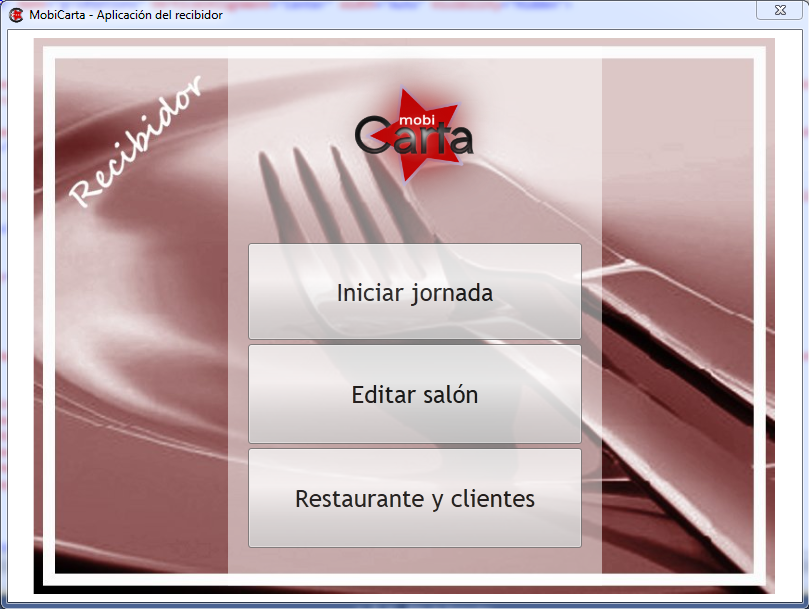
\includegraphics[width=0.8\textwidth]{rcv-main.png}
      \caption{Vista del menú inicial de la aplicación del recibidor.}
      \label{fig:rcv-main}
    \end{center}
  \end{figure}

Esta ventana muestra las tres opciones principales de la aplicación:

\subsubsection{Iniciar jornada}
Es la opción principal de la aplicación. Permite realizar un seguimiento del
estado de las mesas durante una jornada de trabajo. Al seleccionar esta
opción, aparece una ventana vacía con una barra de herramientas que contiene
dos opciones: \emph{Nueva jornada} y \emph{Cargar jornada}.

\begin{itemize}
\item La primera opción (figura \ref{fig:rcv-JourneyNew}), permite iniciar una
nueva jornada de trabajo, a partir de la selección de una de las plantillas
disponibles para el restaurante:

  \begin{figure}[h]
    \begin{center}
      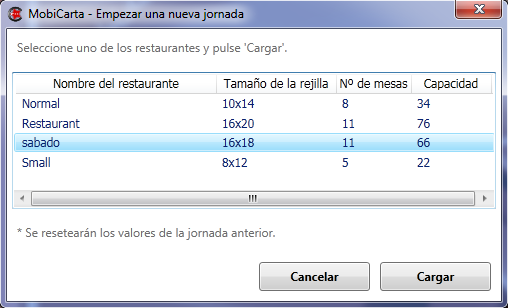
\includegraphics[width=0.6\textwidth]{rcv-JourneyNew.png}
      \caption{Inicio de una nueva jornada.}
      \label{fig:rcv-JourneyNew}
    \end{center}
  \end{figure}

Al seleccionar esta opción, se carga la plantilla seleccionada y se reinicia
el estado de las mesas, apareciendo todas ellas como \textbf{libres} (de
color blanco) (figura \ref{fig:rcv-JourneyWhite}):

  \begin{figure}[ht]
    \begin{center}
      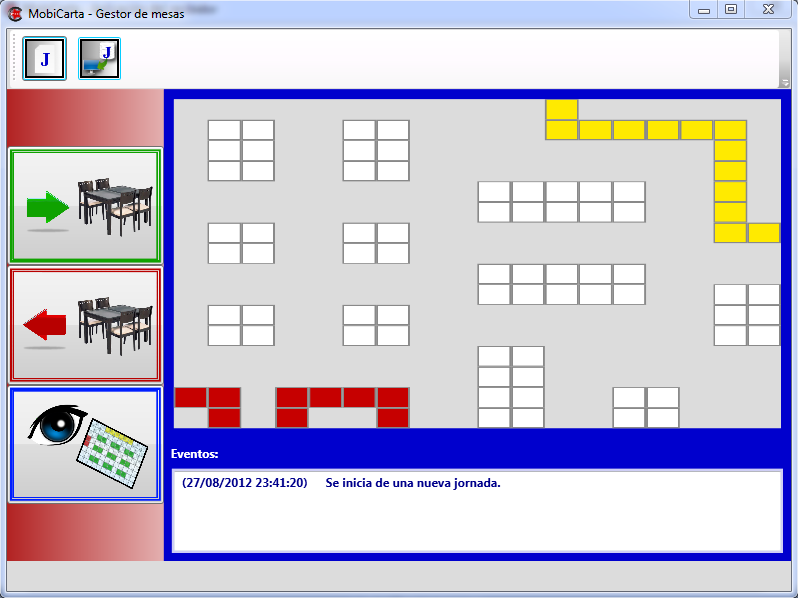
\includegraphics[width=1\textwidth]{rcv-JourneyWhite.png}
      \caption{Vista general del gestor de mesas del restaurante.}
      \label{fig:rcv-JourneyWhite}
    \end{center}
  \end{figure}

Las casillas rojas representan la posición que ocupa el recibidor, mientras
que las amarillas representan la posición que ocupa la barra en el restaurante.

\item La segunda opción (\emph{Cargar jornada}), permite recuperar los datos
de la jornada anterior. Es decir, permite recuperar la situación que tenía el
restaurante antes de cerrar por última vez la aplicación. En este caso sólo
se mostrará la plantilla utilizada en la jornada anterior.
\end{itemize}

Durante la ejecución de una jornada de trabajo (\emph{nueva} o
\emph{recuperada}) se dispone de tres opciones:
\begin{itemize}
\item Opción \textbf{\emph{Ha llegado un cliente}}. Para registrar la llegada
de un cliente tradicional (\emph{no \acs{NFC}}), se seleccionará esta opción.
A continuación, aparecerá la ventana mostrará una interfaz como la de la 
figura \ref{fig:rcv-JourneyNewClient}. Dicha interfaz muestra un identificador
de usuario (generado automáticamente) que representará al cliente durante su
estancia en el restaurante. Además, también muestra un teclado numérico a
través del cual se seleccionará el número de comensales que son en total.

  \begin{figure}[ht]
    \begin{center}
      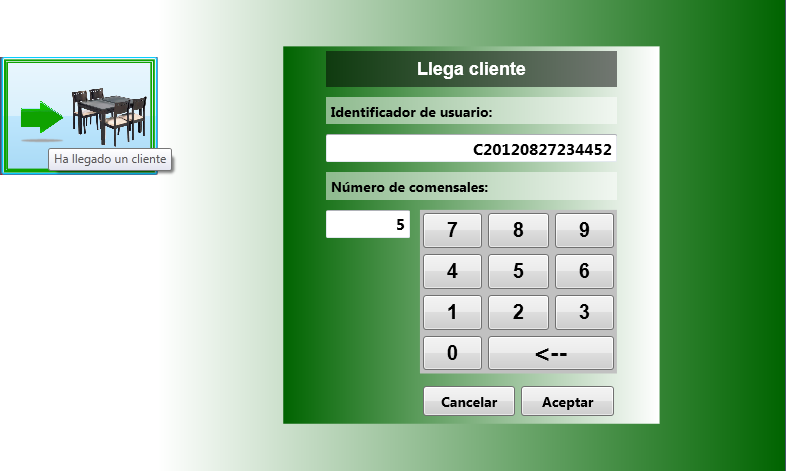
\includegraphics[width=0.9\textwidth]{rcv-JourneyNewClient.png}
      \caption{Opción \emph{Ha llegado un cliente}.}
      \label{fig:rcv-JourneyNewClient}
    \end{center}
  \end{figure}

Una vez determinados identificador y número de comensales, se pulsa
\emph{Aceptar}. A continuación, aparecerá una plantilla del restaurante que
informa del estado de sus mesas (figura \ref{fig:rcv-JourneyAlloc}):

  \begin{figure}[ht]
    \begin{center}
      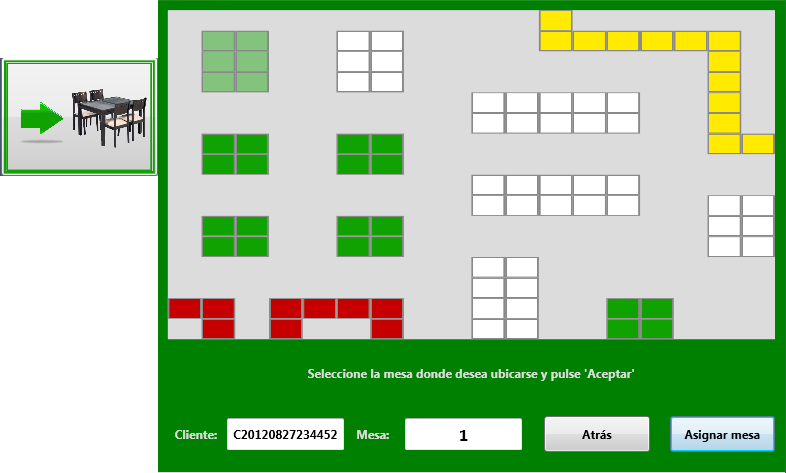
\includegraphics[width=0.9\textwidth]{rcv-JourneyAlloc.png}
      \caption{Seleccionando la mesa para un cliente recien llegado.}
      \label{fig:rcv-JourneyAlloc}
    \end{center}
  \end{figure}

  \begin{itemize}
  \item Las casillas de \textbf{color blanco}, simbolizan a aquellas mesas que
  están libres y además tienen una capacidad suficiente como para albergar
  al número de comensales especificados en el paso anterior. Es decir, son las
  mesas \emph{disponibles}.
  \item Las casillas de \textbf{color verde}, simbolizan a aquellas mesas que
  están ocupadas o que simplemente no tienen una capacidad suficiente como para
  alojar a los nuevos comensales. Es decir, son mesas \emph{no disponibles}.
  \item Al seleccionar una de las mesas blancas, su estado cambiará a
  \textbf{color verde claro} para resaltarla entre las demás mesas
  \emph{libres}. Para confirmar la asignación de una mesa hay que seleccionar
  el botón \emph{Asignar mesa}.
  \end{itemize}

Cuando llega un cliente \acs{NFC}, no hace falta seleccionar la opción
\emph{Ha llegado un cliente}, sino que, cuando el dispositivo móvil del
cliente conecta con esta aplicación se muestra una interfaz similar a la
de la figura \ref{fig:rcv-JourneyNewClient}, pero esta vez con los datos
personalizados del cliente \acs{NFC} (figura
\ref{fig:rcv-JourneyNewClientNFC}).

  \begin{figure}[ht]
    \begin{center}
      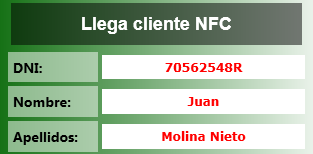
\includegraphics[width=0.5\textwidth]{rcv-JourneyNewClientNFC.png}
      \caption{Ha llegado un cliente \acs{NFC}.}
      \label{fig:rcv-JourneyNewClientNFC}
    \end{center}
  \end{figure}

Una vez especificado del número de comensales, se pulsa \emph{Aceptar} y
se elige una de las mesas \emph{libres}, como se hizo en el caso del
cliente tradicional.

\item Opción \textbf{\emph{El cliente se va}}. Para registrar la salida de un
cliente tradicional (no \acs{NFC}), se seleccionará esta opción. A
continuación, aparecerá la plantilla con el estado de las mesas (figura
\ref{fig:rcv-JourneyDealloc}).

  \begin{figure}[ht]
    \begin{center}
      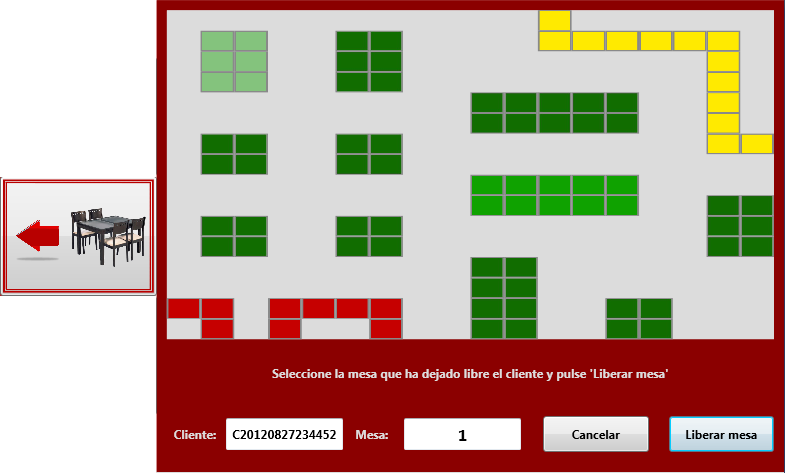
\includegraphics[width=0.9\textwidth]{rcv-JourneyDealloc.png}
      \caption{Seleccionando la mesa de un cliente que se va.}
      \label{fig:rcv-JourneyDealloc}
    \end{center}
  \end{figure}

  \begin{itemize}
  \item Las casillas de color \textbf{verde oscuro}, simbolizan las mesas que
  han realizado algún pedido y todavía no lo han pagado.
  \item Las casillas de color \textbf{naranja}, simbolizan las mesas que han
  pagado todos sus pedidos.
  \item Y las casillas de color \textbf{verde}, simbolizan las mesas que
  todavía no han realizado ningún pedido.
  \end{itemize}

  Las mesas de color \textbf{naranja} y \textbf{verde} serán las candidatas a
  ser desalojadas, en el primer caso, porque ya han pagado lo que debían; y en
  el segundo, porque no deben nada. La mesa seleccionada cambiará a
  \textbf{color verde claro}. Y para confirmar que esa mesa ha quedado libre
  se pulsa el botón \emph{Liberar mesa}.

Cuando un cliente \acs{NFC} notifica su salida y ya ha pagado (de forma
tradicional) sus pedidos, aparecerá automáticamente la siguiente interfaz 
(figura \ref{fig:rcv-JourneyExitNFC}).

  \begin{figure}[ht]
    \begin{center}
      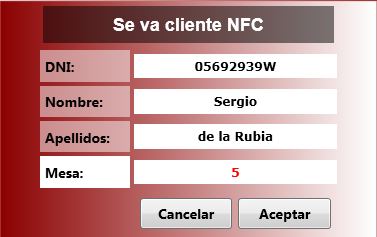
\includegraphics[width=0.5\textwidth]{rcv-JourneyExitNFC.png}
      \caption{Se marcha cliente \acs{NFC}.}
      \label{fig:rcv-JourneyExitNFC}
    \end{center}
  \end{figure}

Para liberar su mesa, simplemente hay que pulsar \emph{Aceptar}.

\item Opción \textbf{\emph{Vista general}}. Esta opción muestra la plantilla
actualizada del estado de las mesas del restaurante. En principio, cada vez que 
el usuario la pulsa, la aplicación hace una petición al servicio web para que 
compruebe el estado de las mesas. Aunque, si el usuario mantiene esta vista,
será actualizará automáticamente cada 30 segundos.

  \begin{figure}[ht]
    \begin{center}
      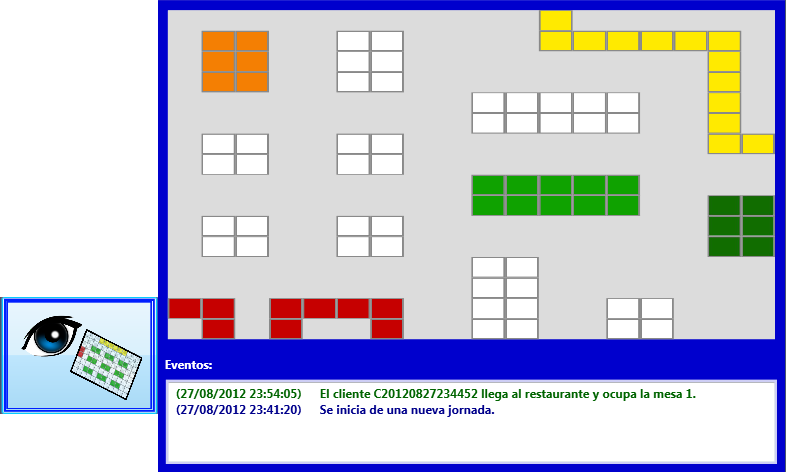
\includegraphics[width=0.9\textwidth]{rcv-JourneyView.png}
      \caption{Opción \emph{Vista general} del restaurante.}
      \label{fig:rcv-JourneyView}
    \end{center}
  \end{figure}

La leyenda de colores es similar a la vista en las opciones anteriores:
  \begin{itemize}
  \item Las casillas de \textbf{color rojo}, simbolizan la ubicación del
  recibidor.
  \item Las casillas de \textbf{color amarillo}, simbolizan la ubicación de la
  barra.
  \item Las casillas de \textbf{color blanco}, representan a las mesas vacías.
  \item Las casillas de \textbf{color verde}, representan a las mesas ocupadas
  que aún no han realizado ningún pedido.
  \item Las casillas de \textbf{color verde oscuro}, representan a las mesas
  ocupadas que han realizado algún pedido.
  \item Y las casillas de \textbf{color naranja}, representan a las mesas que
  han pagado sus pedidos.
  \end{itemize}

\item Una cuarta opción sería: \textbf{\emph{Paga cliente \acs{NFC}}}, pero
esta opción no es directamente seleccionable desde la aplicación.

Cuando un cliente \acs{NFC} ha realizado varios pedidos, no los ha pagado de
forma tradicional y desea abandonar el restaurante, activa el cobro mediante 
\acs{NFC} (figura \ref{fig:rcv-JourneyNFCPay}):

  \begin{figure}[ht]
    \begin{center}
      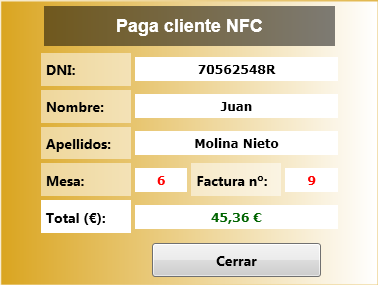
\includegraphics[width=0.5\textwidth]{rcv-JourneyNFCPay.png}
      \caption{Pago de un cliente por \acs{NFC}.}
      \label{fig:rcv-JourneyNFCPay}
    \end{center}
  \end{figure}

La operación es gestionada automáticamente por la apliación, que finalmente
muestra el resultado.
\end{itemize}

\subsubsection{Editar salón}
Esta opción permite editar las plantillas de restaurante usadas en el
transcurso de una jornada. Al seleccionarla aparece una ventana como la de
la figura \ref{fig:rcv-editor}:

  \begin{figure}[ht]
    \begin{center}
      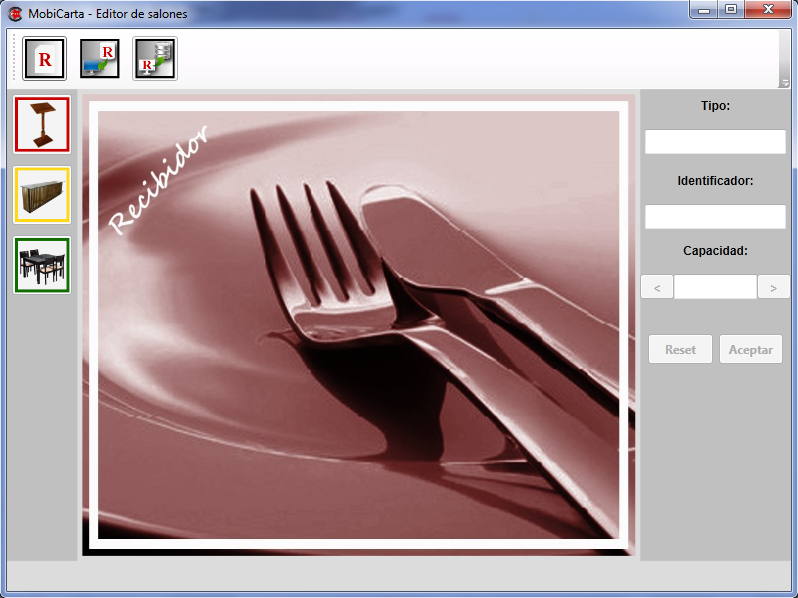
\includegraphics[width=1\textwidth]{rcv-editor.png}
      \caption{Vista inicial del editor de salones.}
      \label{fig:rcv-editor}
    \end{center}
  \end{figure}

Esta ventana tiene una barra de herramientas con tres opciones:
\begin{itemize}
\item \textbf{Nuevo restaurante} (figura \ref{fig:rcv-editorNew}). Genera
una plantilla en blanco, a partir de un nombre, un número de filas y un
número de columnas (que determinan el tamaño de la rejilla de la plantilla).

  \begin{figure}[ht]
    \begin{center}
      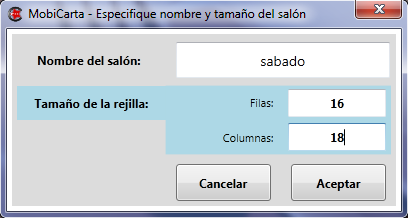
\includegraphics[width=0.5\textwidth]{rcv-editorNew.png}
      \caption{Creando una nueva plantilla para el restaurante.}
      \label{fig:rcv-editorNew}
    \end{center}
  \end{figure}

\item \textbf{Cargar restaurante}. Permite cargar de la base de datos, las 
plantillas creadas y guardadas con anterioridad.
\item \textbf{Guardar restaurante}. Permite guardar en la base de datos, la 
plantilla creada o modificada por el editor.
\end{itemize}

La figura \ref{fig:rcv-editorEdit} muestra un ejemplo de edición de plantilla
para un restaurante.

  \begin{figure}[ht]
    \begin{center}
      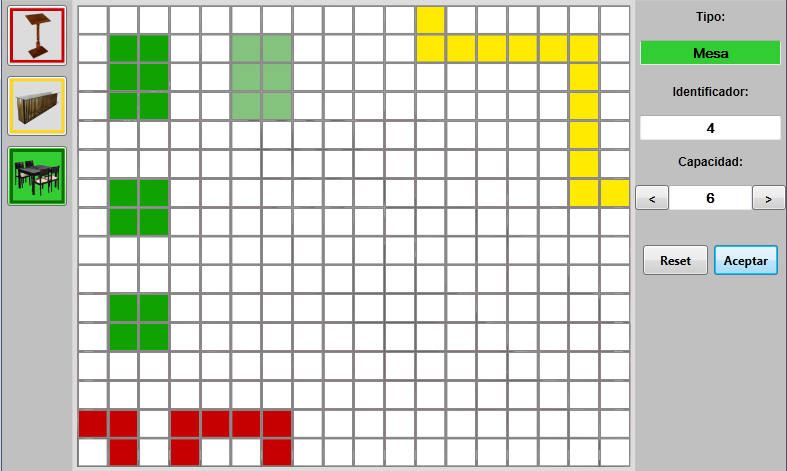
\includegraphics[width=0.9\textwidth]{rcv-editorEdit.png}
      \caption{Editando una plantilla con el editor de salones.}
      \label{fig:rcv-editorEdit}
    \end{center}
  \end{figure}

Para colocar objetos dentro de la plantilla basta con:
\begin{itemize}
\item Seleccionar uno de los tres objetos de la barra de herramientas de la
izquierda: \textbf{recibidor} (rojo), \textbf{barra} (amarillo) o \textbf{mesa}
(verde).
\item En la barra de la derecha aparecen los atributos del objeto que se va a
colocar. En caso de tratarse de una mesa, al objeto se le asignará un 
identificador único y una capacidad (que puede ser editada).
\item Mientras permanece alguno de los objetos seleccionados es posible hacer
click sobre las casillas de la plantilla. Con ello se determina la ubicación
del objeto dentro del restaurante.
\item Para confirmar la ubicación del objeto en la plantilla, es necesario
pulsar el botón \emph{Aceptar} (en la barra de herramientas de la derecha).
\item Si por el contrario se quiere cancelar dicha ubicación, se pulsará la
opción \emph{Reset}.
\item Los objetos que no han sido confirmados aparecen con la misma tonalidad 
(según el tipo) que los objetos confirmados, pero con un color más apagado.
\end{itemize}

\subsubsection{Restaurante y clientes}
Esta última opción, permite consultar los datos propios del restaurante y
de los clientes. Al seleccionar esta opción se abre una ventana que cuenta
con una barra de herramientas con las siguientes opciones:
\begin{itemize}
\item \textbf{Cargar datos del restaurante}. Esta opción se encarga de
solicitar al servicio web los datos del restaurante, para su representación
en pantalla (figura \ref{fig:rcv-statsRest}).

  \begin{figure}[ht]
    \begin{center}
      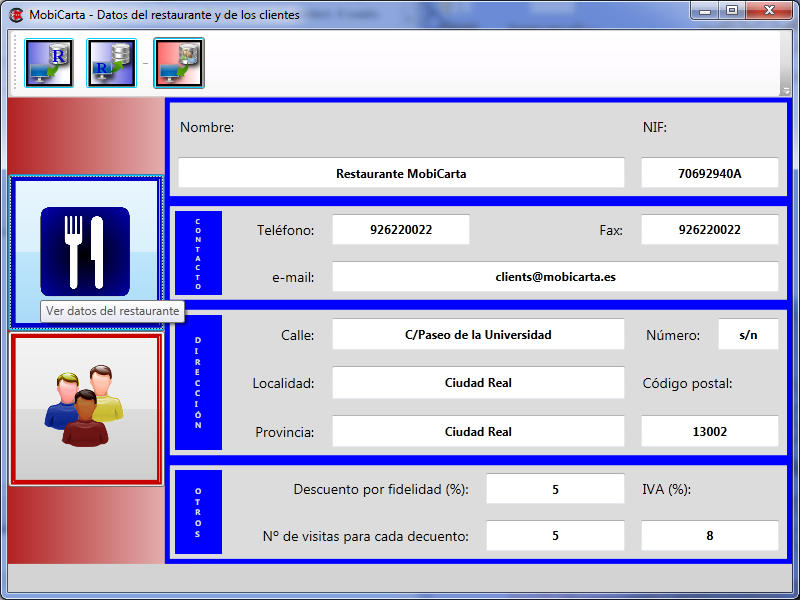
\includegraphics[width=0.9\textwidth]{rcv-statsRest.png}
      \caption{Vista de los datos del restaurante.}
      \label{fig:rcv-statsRest}
    \end{center}
  \end{figure}

Los datos cargados pueden ser editados.
\item \textbf{Guardar datos del restaurante}. Si se ha realizado algún cambio
en los datos del restaurante, esta es la opción que permite guardarlos. Esta
opción envía los nuevos datos al servicio web para que actualice la base de
datos.
\item \textbf{Cargar lista de clientes}. Además de los datos del restaurante,
también es posible consultar los datos de los clientes del restaurante. Esta
opción carga una lista con los usuarios que han visitado el restaurante en
alguna ocasión y muestra otros parámetros como: su estado (Activo o no activo,
dependiendo de que se encuentren o no dentro del restaurante), su DNI o
identificador, su nombre y apellidos (para clientes \acs{NFC}) y el número
de apariciones (figura \ref{fig:rcv-statsClients}):

  \begin{figure}[ht]
    \begin{center}
      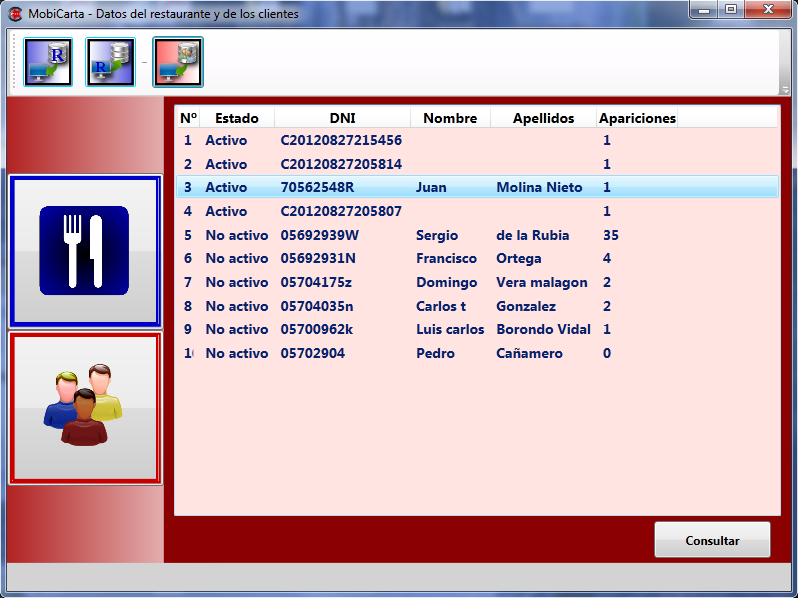
\includegraphics[width=0.9\textwidth]{rcv-statsClients.png}
      \caption{Vista de los clientes del restaurante.}
      \label{fig:rcv-statsClients}
    \end{center}
  \end{figure}

Si se selecciona a alguno de los clientes y se pulsa consultar, aparece
información más detallada del cliente (figura \ref{fig:rcv-statClient}):

  \begin{figure}[H]
    \begin{center}
      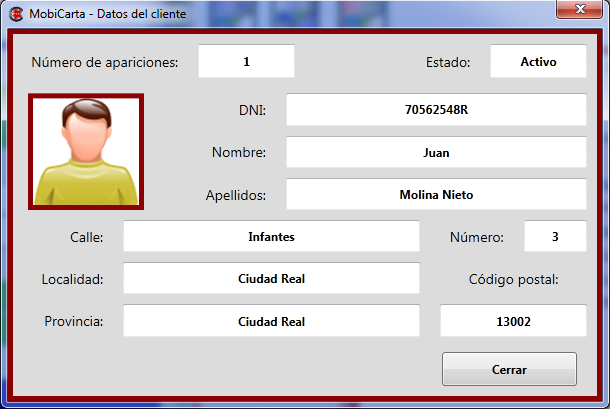
\includegraphics[width=0.7\textwidth]{rcv-statClient.png}
      \caption{Vista del perfil de un cliente \acs{NFC}.}
      \label{fig:rcv-statClient}
    \end{center}
  \end{figure}
\end{itemize}

Los botones de la barra de herramientas de la izquierda, permiten alternar
entre la vista de los datos del restaurante y la vista de la lista de clientes.


\subsection{Aplicación de la barra}
Al igual que la del \emph{recibidor}, la \emph{apliación de la barra} es una
aplicación de escritorio diseñada para ser ejecutada sobre sistemas
\texttt{Windows}. Para iniciar su ejecución, basta con tenerla instalada y
hacer doble click sobre el archivo \texttt{Bar.exe}. El equipo donde se
ejecute debe contar con conectividad \texttt{Bluetooth} y conexión a
Internet; y debe conocer donde se encuentran alojados los servicios web.

La \emph{aplicación de la barra} está diseñada para facilitar la realización de
las siguientes tareas:
\begin{itemize}
\item Tomar nota de los pedidos de los clientes. Tanto de forma manual, para
clientes tradicionales; como de forma automática vía \texttt{Bluetooth}, para
clientes \acs{NFC}.
\item Gestionar el estado de dichos pedidos.
\item Gestionar la cartera de productos y categorías de productos del
restaurante.
\item Mecanizar las facturas de las mesas atendidas.
\item Recuperar el histórico de facturas y pedidos del restaurante.
\end{itemize}

Una vez inicida la aplicación, aparece una ventana como la que muestra la
figura \ref{fig:bar-main}:

  \begin{figure}[H]
    \begin{center}
      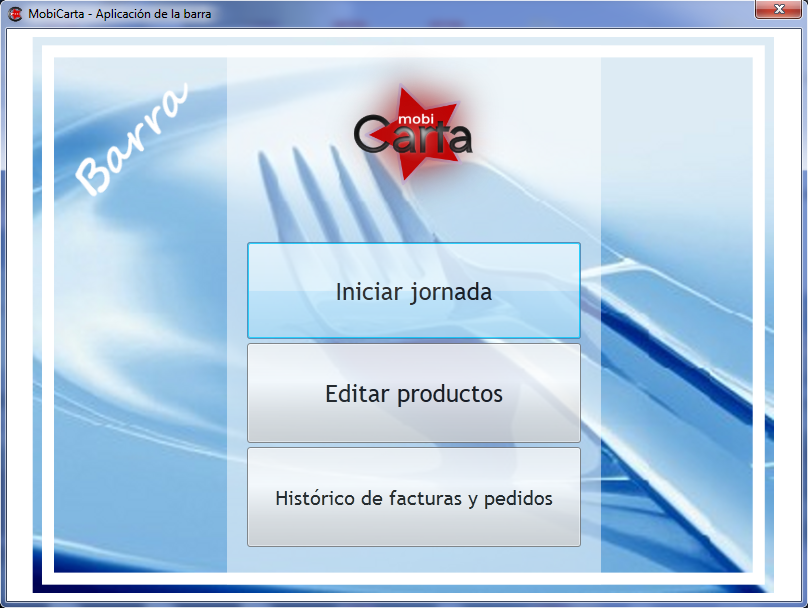
\includegraphics[width=0.8\textwidth]{bar-main.png}
      \caption{Vista del menú inicial de la aplicación de la barra.}
      \label{fig:bar-main}
    \end{center}
  \end{figure}

Esta ventana muestra las tres opciones principales de la aplicación:

\subsubsection{Iniciar jornada}
Es la opción principal de la aplicación. Permite realizar un seguimiento de los
pedidos que se van realizando a lo largo de una jornada de trabajo.

Al seleccionar esta opción, se abre una nueva ventana. Esta ventana tiene un
aspecto similar a la de la \emph{aplicación del recibidor} y también cuenta
con una barra de herramientas superior con dos opciones:
\begin{itemize}
\item \textbf{Nueva jornada}.
\item \textbf{Cargar jornada}.
\end{itemize}
La funcionalidad de estas opciones es la misma que la explicada en la sección
\emph{Iniciar jornada} de la \emph{aplicación del recibidor}.

Si, en este caso, se inicia una \emph{jornada existente}, la ventana del gestor 
de pedidos mostrará una apariencia similar a la de la figura
\ref{fig:bar-JourneyNew}:

  \begin{figure}[H]
    \begin{center}
      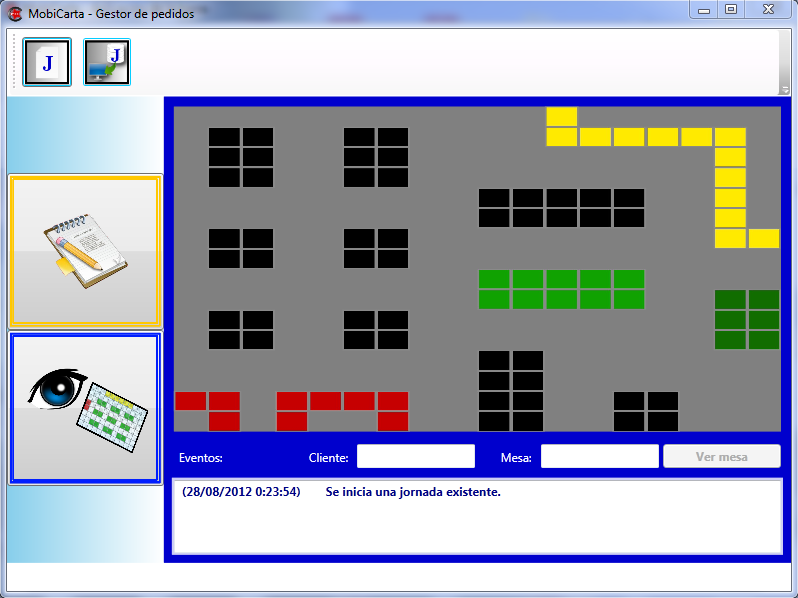
\includegraphics[width=\textwidth]{bar-JourneyNew.png}
      \caption{Vista general de la plantilla del gestor de pedidos.}
      \label{fig:bar-JourneyNew}
    \end{center}
  \end{figure}

Como puede observarse, al cargarse una jornada previamente abierta, el estado 
de las mesas va a ser no va a ser el inicial, en la mayor parte de los casos.

A diferencia de la \emph{aplicación del recibidor}, la barra de herramientas de 
la izquierda de esta aplicación cuenta con dos opciones:
\begin{itemize}
\item Opción \emph{Ver pedidos}.

La opción \emph{Ver pedidos}, permite visualizar un listado con el estado de
los pedidos de las mesas ocupadas del restaurante (figura
\ref{fig:bar-JourneyOrders}). Cada pedido contiene la siguiente información:
nombre del \emph{Producto}, \emph{Cantidad} del producto, \emph{Mesa} de
destino, \emph{Fecha} y \emph{Estado}. Según el estado en el que se encuentre
un pedido, aparecerá de un color u otro:
  \begin{itemize}
  \item \textbf{Color blanco}. Significa que el pedido está en estado de
  \emph{no atendido}. Es decir, el pedido ha sido registrado en la lista pero
  ningún camarero ni cocinero se ha hecho cargo de él.
  \item \textbf{Color amarillo}. Representa a los pedidos \emph{atendido}s.
  Un pedido se encuentra \emph{atendido} cuando este necesita ser preparado o
  elaborado antes de ser servido y alguno de los cocineros se está ocupando de 
  esta tarea. En el caso de las bebidas, por ejemplo, no tendría sentido
  utilizar este estado.
  \item \textbf{Color verde}. Representa a los pedidos \emph{servido}s. Un
  pedido que ha llegado a la mesa de destino es un pedido \emph{servido}.
  \item \textbf{Color rojo}. Representa que un pedido está \emph{detenido}.
  Es un estado excepcional que puede utilizarse, por ejemplo, en caso
  de que se sospeche que el pedido ha sido tomado de forma errónea.
  \end{itemize}

  \begin{figure}[H]
    \begin{center}
      \includegraphics[width=0.9\textwidth]{bar-JourneyOrders.png}
      \caption{Opción \emph{Ver pedidos} del gestor de pedidos.}
      \label{fig:bar-JourneyOrders}
    \end{center}
  \end{figure}

Para cambiar el estado de un pedido: primero, se selecciona el pedido en la 
lista; y después, se selecciona el nuevo estado, utilizando para ello los
botones de la mini-barra de herramientas que aparece a la izquierda de la
lista de pedidos.

Además de esta, se tiene otra mini-barra de herramientas sobre la lista de
pedidos. Esta mini-barra tiene las siguientes opciones:
\begin{itemize}
\item \textbf{Nuevo pedido}. Esta opción abre una nueva ventana emergente
(figura \ref{fig:bar-JourneyNewOrder}). La interfaz de esta ventana permite 
tomar nota, de forma manual y bastante intuitiva, de los pedidos de las mesas.

  \begin{figure}[H]
    \begin{center}
      \includegraphics[width=0.9\textwidth]{bar-JourneyNewOrder.png}
      \caption{Ventana que permite anotar, de forma manual, un nuevo pedido.}
      \label{fig:bar-JourneyNewOrder}
    \end{center}
  \end{figure}

Para asignar un nuevo pedido a una mesa, se deben seguir los siguientes pasos:
\begin{enumerate}
\item Se selecciona la mesa de destino, usando para ello la caja desplegable
situada en la parte superior izquierda de la ventana. En esta caja aparecen
sólamente las mesas ocupadas.
\item Se selecciona la categoría del producto que se pretende añadir. Al
seleccionar una categoría, se desplegará una lista con los productos que
pertenecen a dicha categoría.
\item Para añadir un producto al pedido: primero, se selecciona el producto
en cuestión; después, se selecciona la cantidad de productos de ese tipo
(utilizando para ello el teclado numérico que aparece en pantalla) y; por
último, se hace click en \emph{Intro}. En la lista que aparece en la parte
izquierda de la ventana, aparecerá el producto y la cantidad seleccionada.
Si no se especifica el número de productos, se añadirá una unidad del tipo
de producto seleccionado cada vez que se pulse el botón \emph{Intro}.
\item La lista de la izquierda muestra los productos y las cantidades
introducidas. Para decrementar o incrementar el número de unidades de un tipo
de producto basta con: seleccionar uno de los productos de esta lista y
hacer click en los botones ``\emph{+}'' (para incrementarlo) o ``\emph{-}''
(para decrementarlo). Si el producto alcanza las ``0'' unidades, desaparece de 
la lista. Otra forma de quitar un producto es: seleccionarlo de la lista y
hacer click en el botón ``\emph{X}''.
\item Para confirmar el pedido, se hará click en \emph{Aceptar}.
\end{enumerate}

La lista de pedidos que aparece en la opción \emph{Ver pedidos} se actualiza
automáticamente.

\item Para eliminar alguno de los pedidos de la lista de \emph{Ver pedidos}, se 
utilizará la opción \emph{Eliminar pedido}, después de seleccionar dicho
pedido.

\item La tercera opción es \emph{Editar pedido}. Para modificar alguno de los
parámetros de un pedido: primero, se seleccionará dicho pedido; y después, se
hará click sobre esta opción. A continuación, aparece una ventana emergente
como la que muestra la figura \ref{fig:bar-JourneyEditOrder}.

  \begin{figure}[H]
    \begin{center}
      \includegraphics[width=0.6\textwidth]{bar-JourneyEditOrder.png}
      \caption{Ventana emergente de edición de pedidos.}
      \label{fig:bar-JourneyEditOrder}
    \end{center}
  \end{figure}

Esta ventana permite modificar la cantidad de productos de ese tipo, la mesa
de destino o el estado del pedido. Para confirmar el cambio se pulsará
\emph{Aceptar}.
\end{itemize}

\item Opción \textbf{Vista general}.

Esta opción abre una vista como la de la figura \ref{fig:bar-JourneyView}.
Su funcionalidad es similar a la de su homónima de la \emph{aplicación del 
recibidor}. Aunque conviene puntualizar dos aspectos:

\begin{itemize}
\item La leyenda de colores no es exactamente la misma:
  \begin{itemize}
  \item Las mesas que no están ocupadas aparecen de \textbf{color negro}.
  \item Las mesas que tienen algún pedido \emph{no servido} aparecen de color
  \textbf{blanco}.
  \item Y las mesas con todos los pedidos \emph{servido}s aparecen de color
  \textbf{verde oscuro}.
  \item El resto de colores representan los mismos estados que en la aplicación
  del recibidor.  
  \end{itemize}

  \begin{figure}[H]
    \begin{center}
      \includegraphics[width=0.9\textwidth]{bar-JourneyView.png}
      \caption{Opción \emph{Vista general} del restaurante.}
      \label{fig:bar-JourneyView}
    \end{center}
  \end{figure}

\item La interfaz permite seleccionar una mesa ocupada para ver su estado.
Al seleccionar una mesa, esta cambia a un color \textbf{verde claro}.
Si se selecciona después el botón \emph{Ver mesa}, se abrirá una interfaz
similar a la de la figura \ref{fig:bar-JourneyTable}.

Esta interfaz tiene un aspecto similar a la mostrada por la opción
\emph{Ver pedidos}, salvo que en esta ocasión aparecen sólamente los pedidos
asignados a esta mesa. Además, en la parte inferior, se muestra información
del cliente que está ocupando la mesa y de la mesa propiamente dicha.
Uno de los atributos de la mesa es el \emph{estado}. Los estados de la mesa
son los mismos que los que se describen en la leyenda de colores utilizados en 
la plantilla del restaurante, es decir: \emph{vacía}, \emph{ocupada},
\emph{esperando pedido}, \emph{servida} y \emph{cobrada}.

Cuando una mesa está \emph{servida}, o lo que es lo mismo, cuando una mesa
tiene todos los pedidos como \emph{servido}s. Se habilita la opción de
\emph{Facturar}. Esta opción produce una petición al servicio web para que
este genere la factura para la mesa. El servicio web devuelve la descripción
detallada de la factura generada para que la aplicación la represente en
una ventana como la siguiente (figura \ref{fig:bar-JourneyBill}).

  \begin{figure}[H]
    \begin{center}
      \includegraphics[width=0.9\textwidth]{bar-JourneyTable.png}
      \caption{Vista del estado de una mesa.}
      \label{fig:bar-JourneyTable}
    \end{center}
  \end{figure}

  \begin{figure}[H]
    \begin{center}
      \includegraphics[width=0.9\textwidth]{bar-JourneyBill.png}
      \caption{Factura de la \emph{mesa 6}, a nombre de \emph{Juan Molina
      Nieto}.}
      \label{fig:bar-JourneyBill}
    \end{center}
  \end{figure}

Al hacer click sobre el botón \emph{PAGADA}, dicho botón quedará desactivado, 
los pedidos de la mesa cambiarán de estado a \emph{Pagado} y la mesa cambiará
su estado a \emph{Cobrada}. Mientras el cliente no salga del restaurante,
dicha factura podrá consultarse a través de la vista de su mesa, pulsando
el botón \emph{Ver factura} (que antes tenía el nombre de \emph{Facturar}).
\end{itemize}
\end{itemize}

\subsubsection{Editar productos}
Esta segunda opción, permite visualizar los productos con los que trabaja el 
restaurante.

Para cargar los productos de la base de datos, se selecciona la opción
\emph{Cargar lista de categorías y productos}, de la barra de herramientas.
La ventana mostrará entonces un aspecto similar a la que aparece en la figura 
\ref{fig:bar-products}:

  \begin{figure}[H]
    \begin{center}
      \includegraphics[width=0.9\textwidth]{bar-products.png}
      \caption{Ventana que muestra la lista de productos del restaurante.}
      \label{fig:bar-products}
    \end{center}
  \end{figure}

Los productos aparecen agrupados por categorías, de tal manera que, para ver
los productos de una categoría, hay que hacer click en dicha categoría.

Tanto la lista de categorías como la de productos puede ser modificada. Para
ello, se cuenta con tres opciones para cada una: \emph{Añadir}, \emph{Eliminar}
y \emph{Editar}:

\begin{itemize}
\item Para \emph{eliminar} una categoría, basta con seleccionar esa categoría y 
pulsar la opción \emph{Eliminar categoría}. Si se elimina una categoría se 
eliminarán todos los productos de dicha categoría.
\item La \emph{edición} de una categoría funciona de la misma forma. En este
caso, sus productos también cambiarán el nombre de su categoría.
\item Cuando se \emph{añade} una categoría (figura
\ref{fig:bar-productsNewCat}), dicha categoría no contendrá (de inicio) ningún
producto.

  \begin{figure}[H]
    \begin{center}
      \includegraphics[width=0.4\textwidth]{bar-productsNewCat.png}
      \caption{Creación de una categoría llamada \emph{Bebidas}.}
      \label{fig:bar-productsNewCat}
    \end{center}
  \end{figure}

\end{itemize}

Para \emph{eliminar}, \emph{editar} o \emph{añadir} un producto, se seguirá
la misma mecánica, pero utilizando los botones \emph{Eliminar producto},
\emph{Editar producto} y \emph{Añadir producto} (ver figura
\ref{fig:bar-productsNewProd}), respectivamente.

  \begin{figure}[H]
    \begin{center}
      \includegraphics[width=0.6\textwidth]{bar-productsNewProd.png}
      \caption{Creación del producto \emph{Fanta de Naranja 200ml}, en la
      categoría \emph{Bebidas}.}
      \label{fig:bar-productsNewProd}
    \end{center}
  \end{figure}

Cabe destacar, que uno de los campos con los que cuenta un producto es el de
\emph{Palabras clave}. En este campo el usuario especificará una serie de
palabras (separadas por comas) que definan mejor al producto. Estas palabras
serán utilizadas por el recomendador a la hora de calcular la similitud entre
este y los demás productos.

Para visualizar un producto recién añadido, bastará con seleccionar la 
categoría a la que se ha inscrito.

\subsubsection{Histórico de facturas y pedidos}
Esta tercera opción permite consultar el historial de facturas del
restaurante, así como también los pedidos que han sido cobrados en dichas
facturas.

La barra de herramientas de la ventana \emph{Histórico de facturas y pedidos}
tiene dos botones:
\begin{itemize}
\item \textbf{Cargar lista de facturas} abre una ventana emergente como
la de la figura \ref{fig:bar-statisticsConsult}. 

  \begin{figure}[H]
    \begin{center}
      \includegraphics[width=0.5\textwidth]{bar-statisticsConsult.png}
      \caption{Ventana emergente para la configuración de la consulta.}
      \label{fig:bar-statisticsConsult}
    \end{center}
  \end{figure}

  \begin{figure}[H]
    \begin{center}
      \includegraphics[width=0.9\textwidth]{bar-statistics.png}
      \caption{Vista del histórico de facturas del restaurante.}
      \label{fig:bar-statistics}
    \end{center}
  \end{figure}

A través de esta ventana se selecciona el número de facturas que se desea 
cargar y el orden (\emph{descendente} o \emph{ascendente}) de dichas facturas. 
Las facturas están ordenadas por su identificador, de tal forma que si se 
seleccionan 10 facturas en orden descendente, se obtendrán las 10 últimas 
facturas generadas. Al pulsar \emph{Aceptar} la ventana principal mostrará
una lista similar a la de la figura \ref{fig:bar-statistics}.

Esta vista permite seleccionar una de las facturas de la lista para verla en
detalle (pulsando el botón \emph{Consultar}). La ventana que se abre es
similar a la de facturación de una mesa (figura \ref{fig:bar-JourneyBill}).

\item \textbf{Cargar lista de pedidos} abre una ventana emergente similar a
la ya vista en la figura \ref{fig:bar-statisticsConsult}. En este caso
hay que tener en cuenta que los pedidos están ordenados por la fecha en la
que se realizaron.

  \begin{figure}[H]
    \begin{center}
      \includegraphics[width=0.9\textwidth]{bar-statisticsOrders.png}
      \caption{Vista del histórico de pedidos del restaurante.}
      \label{fig:bar-statisticsOrders}
    \end{center}
  \end{figure}
\end{itemize}

La figura \ref{fig:bar-statisticsOrders} muestra un ejemplo del resultado
obtenido al consultar el histórico de pedidos del restaurante.

Los botones de la barra de herramientas de la izquierda, permiten alternar 
entre la vista del historial de facturas y la vista del historial de pedidos.

\subsection{Aplicación móvil}
La \emph{aplicación móvil} es un \texttt{MIDlet} diseñado para su ejecución 
sobre la máquina virtual \acs{KVM} de un dispositivo móvil con perfil
\texttt{Java} \acs{CLDC} 1.1 o superior. El dispositivo además debe contar
con las tecnologías inalámbricas \acs{NFC} y \texttt{Bluetooth}.

\subsubsection{Instalación}
La instalación de aplicaciones \texttt{Java} es muy sencilla. Simplemente con
enviar los archivos: \emph{MobiCarta.jar} y \emph{MobiCarta.jad}, la aplicación
aparecerá en la lista de aplicaciones del dispositivo (figura
\ref{fig:mobile-init}).

  \begin{figure}[H]
    \begin{center}
      \includegraphics[width=0.4\textwidth]{mobile-init.png}
      \caption{Aplicación \texttt{MobiCarta} dentro de la sección de 
      aplicaciones del dispositivo móvil.}
      \label{fig:mobile-init}
    \end{center}
  \end{figure}

Sin embargo, muchas de las operaciones que realiza la aplicación van a
solicitar los permisos del usuario para efectuarse, afectando al grado de
automaticidad de las operaciones. Por ello, antes de empezar a utilizar la 
aplicación, conviene cambiar manualmente esos permisos.

Los permisos que hay que cambiar son tres\footnote{Para acceder a los permisos 
de la aplicación hay que pulsar la opción \emph{Opciones} cuando el selector de 
aplicaciones está, en este caso, sobre la aplicación \texttt{MobiCarta}.}:
\begin{itemize}
\item \emph{Comunicación - Conectividad - Siempre permitida}.
\item \emph{Acceso a datos - Lectura de datos de usuario - Siempre permitida}.
\item y \emph{Acceso a datos - Añadir y editar datos de usuario - Siempre
permitida}.
\end{itemize}

Por último, como la aplicación va a trabajar con los datos personales del
usuario, antes de realizar cualquier acción con la aplicación móvil, conviene
rellenar el formulario del \emph{perfil del cliente}. Este formulario se
encuentra en la opción \emph{Perfil} de la pantalla principal de la aplicación.
El primer acceso a este formulario generará un aviso como el siguiente
(figura \ref{fig:mobile-form}):

  \begin{figure}[H]
    \begin{center}
      \includegraphics[width=0.4\textwidth]{mobile-form.png}
      \caption{Aviso de: \emph{Complete el siguiente formulario}.}
      \label{fig:mobile-form}
    \end{center}
  \end{figure}

Y, a continuación, aparecerá el formulario (figura \ref{fig:mobile-profile}):

  \begin{figure}[H]
    \begin{center}
      \includegraphics[width=0.4\textwidth]{mobile-profile.png}
      \caption{Formulario del perfil del cliente.}
      \label{fig:mobile-profile}
    \end{center}
  \end{figure}

Una vez completados todos los campos del formulario, se seleccionará la
opción \emph{Guardar}. Si los datos introducidos son correctos, se codificarán 
en formato \acs{XML} y serán almacenados en un archivo llamado
\texttt{profile.xml}, que se encontrará en la carpeta \emph{mobiCarta} de la 
memoria extraíble del dispositivo (figura \ref{fig:mobile-profileSave}).

  \begin{figure}[H]
    \begin{center}
      \includegraphics[width=0.4\textwidth]{mobile-profileSave.png}
      \caption{Aviso de: \emph{El perfil ha sido guardado satistactoriamente}.}
      \label{fig:mobile-profileSave}
    \end{center}
  \end{figure}

Este último paso dará por finalizada la configuración de la aplicación.

A continuación, se explican las principales funcionalidades de la aplicación:

\subsubsection{Registrar la entrada del cliente}
Para registrar la entrada en el restaurante, el usuario debe buscar una
etiqueta de tipo \textbf{app/checkpoint} (ver \emph{Definición de las etiquetas 
\acs{RFID} utilizadas}, Anexo \ref{chap:tags}). Esta etiqueta debe encontrarse
próxima al terminal donde se encuentra el recibidor (o \emph{maître}). Cuando
el usuario toque con su dispositivo móvil dicha etiqueta, la aplicación
\texttt{MobiCarta} se abrirá automáticamente y mostrará el siguiente
mensaje (figura \ref{fig:mobile-connecting}):

  \begin{figure}[H]
    \begin{center}
      \includegraphics[width=0.4\textwidth]{mobile-connecting.png}
      \caption{Conectando con el servicio \texttt{Bluetooth} de la
      \emph{aplicación del recibidor}.}
      \label{fig:mobile-connecting}
    \end{center}
  \end{figure}

La aplicación intentará contactar con el servicio \texttt{Bluetooth} publicado
por la aplicación del recibidor. Cuando esta se produce, la aplicación móvil
carga los datos del perfil del cliente y se los envía al recibidor. Si la
transacción se ha producido de forma satisfactoria, se mostrará el siguiente
mensaje (figura \ref{fig:mobile-registry}):

  \begin{figure}[H]
    \begin{center}
      \includegraphics[width=0.4\textwidth]{mobile-registry.png}
      \caption{Aviso de: \emph{Registro efectuado satisfactoriamente}.}
      \label{fig:mobile-registry}
    \end{center}
  \end{figure}

La aplicación del recibidor por su parte, enviará las recomendaciones
generadas para el usuario. Entre ellas, está este mensaje de bienvenida
(figura \ref{fig:mobile-welcome}):

  \begin{figure}[H]
    \begin{center}
      \includegraphics[width=0.4\textwidth]{mobile-welcome.png}
      \caption{Mensaje de bienvenida que además informa del número de visitas
      realizadas y los descuentos disponibles para las siguientes visitas.}
      \label{fig:mobile-welcome}
    \end{center}
  \end{figure}

El resto de recomendaciones (en este caso de productos) serán almacenadas 
en formato \acs{XML} en el archivo \texttt{Recommendations.xml}, también
en la carpeta \emph{mobiCarta}.

El \emph{maître} se encargará de registrar el número de comensales que
acceden al restaurante y la mesa donde se sentarán.

\subsubsection{Realizar pedido}
Una vez que el cliente se ha sentado, tendrá a su alcance una carta con
distintos tipos de etiquetas:

\begin{itemize}
\item Las etiquetas de tipo \textbf{app/product} contendrán la información de 
los productos a los que representan. El contacto del dispositivo móvil con
una etiqueta de este tipo arrancará la aplicación en \emph{Modo pedido},
añadiendo además el producto seleccionado a la lista de productos del pedido.
El usuario irá componiendo su pedido tocando las etiquetas de los productos
que le interesen. Si el usuario selecciona varias veces el mismo producto,
incrementará el número de productos de ese tipo (figura
\ref{fig:mobile-order}):

  \begin{figure}[H]
    \begin{center}
      \includegraphics[width=0.4\textwidth]{mobile-order.png}
      \caption{Pantalla de la lista de productos del pedido. Si se realizan dos 
      pedidos de \emph{Macarrones con tomate}, la segunda unidad tendrá un 
      descuento del 50\% en su precio.}
      \label{fig:mobile-order}
    \end{center}
  \end{figure}

Al arrancar en \emph{Modo pedido}, la aplicación carga el archivo de 
recomendaciones \texttt{Recommendations.xml} almacenado con anterioridad y
extrae de él las recomendaciones para el usuario. Estas recomendaciones son
accesibles a través de la opción \emph{Recomendaciones}. La pantalla de
recomendaciones (figura \ref{fig:mobile-rec}) muestra un listado con: los
productos más consumidos por el cliente, los productos que tienen algún
descuento y los productos recomendados (por su similitud con los productos más
consumidos por el cliente).

  \begin{figure}[H]
    \begin{center}
      \includegraphics[width=1\textwidth]{mobile-rec.png}
      \caption{Pantalla de recomendaciones para el cliente.}
      \label{fig:mobile-rec}
    \end{center}
  \end{figure}

Los productos en promoción, aparecen también en la ventana de la lista de
productos para un pedido (ver figura \ref{fig:mobile-order}).

\item Si, mientras está componiendo la lista del pedido, el usuario se
equivoca tocando un producto que no desea y desea decrementar dicho producto;
la carta dispone también del tipo de etiquetas \textbf{app/subtract-product}.
Para decrementar (en una unidad) un producto:
  \begin{itemize}
  \item primero, se tocará una etiqueta de este tipo.
  \item A continuación, aparecerá el siguiente aviso (figura
  \ref{fig:mobile-decrease}):

  \begin{figure}[H]
    \begin{center}
      \includegraphics[width=0.4\textwidth]{mobile-decrease.png}
      \caption{Aviso de: \emph{Seleccione el producto que desea decrementar}.}
      \label{fig:mobile-decrease}
    \end{center}
  \end{figure}

  \item y después, se seleccionará el producto que se desee decrementar.
  \item La lista de productos se actualizará automáticamente.
  \end{itemize}

\item Por último, las etiquetas de tipo \textbf{app/send-order} servirán
para enviar la lista de productos elaborada a la \emph{aplicación de la barra}.
La aplicación móvil buscará el servicio \texttt{Bluetooth} publicado por la
\emph{aplicación de la barra} (figura \ref{fig:mobile-ordering}). Y, cuando la 
encuentre, enviará el pedido (con el DNI del usuario como identificador).

  \begin{figure}[H]
    \begin{center}
      \includegraphics[width=0.4\textwidth]{mobile-ordering.png}
      \caption{Conectando con el servicio \texttt{Bluetooth} de la
      \emph{aplicación de la barra}.}
      \label{fig:mobile-ordering}
    \end{center}
  \end{figure}

Cuando la \emph{aplicación de la barra} reciba dicho pedido, contestará con
un mensaje como el que muestra la figura \ref{fig:mobile-orderingOk}:

  \begin{figure}[H]
    \begin{center}
      \includegraphics[width=0.4\textwidth]{mobile-orderingOk.png}
      \caption{Aviso de: \emph{Su pedido está en camino\dots}.}
      \label{fig:mobile-orderingOk}
    \end{center}
  \end{figure}

\end{itemize}

\subsubsection{Solicitar factura}
Además de las etiquetas comentadas con anterioridad, la carta dispone también
de un tipo de etiqueta \textbf{app/bill-request}. Esta etiqueta permite 
solicitar (a la \emph{aplicación de la barra}) un resumen de la cuenta que
debe hasta ese momento.

El contacto del dispositivo con una etiqueta de este tipo iniciará la
aplicación en \emph{Modo solicitar factura} (figura
\ref{fig:mobile-billRequest}):

  \begin{figure}[H]
    \begin{center}
      \includegraphics[width=0.4\textwidth]{mobile-billRequest.png}
      \caption{Conectando con el servicio \texttt{Bluetooth} de la
      \emph{aplicación de la barra} para solicitar factura.}
      \label{fig:mobile-billRequest}
    \end{center}
  \end{figure}

La aplicación móvil buscará de nuevo el servicio \texttt{Bluetooth} publicado
por la \emph{aplicación de la barra} y le mandará los datos del cliente que
solicita la factura. La respuesta obtenida será presentada al usuario de
forma similar a la que aparece en la figura \ref{fig:mobile-shortBill}:

  \begin{figure}[H]
    \begin{center}
      \includegraphics[width=1\textwidth]{mobile-shortBill.png}
      \caption{Factura para la \emph{mesa 5}.}
      \label{fig:mobile-shortBill}
    \end{center}
  \end{figure}

\subsubsection{Realizar pago \acs{NFC} y registrar la salida del restaurante}
Cuando un cliente \acs{NFC} desea pagar lo que ha tomado tiene dos opciones:
\begin{itemize}
\item Pagar de la \emph{forma tradicional}. Es decir, al contado o con tarjeta.
Cuando el usuario opte por esta forma de pago, necesitará volver a realizar
el \emph{registro de cliente} (tocando la etiqueta \textbf{app/checkpoint}) en
el terminal del recibidor, para notificar su salida del restaurante. En este 
caso, la aplicación del recibidor le despedirá con un mensajes del tipo:
``\emph{Gracias por su visita}''.
\item Pagar utilizando \acs{NFC}. Cuando el cliente toca la etiqueta
\textbf{app/checkpoint} del recibidor y no ha pagado su cuenta, se inicia el
\emph{modo registro} de cliente. En este caso, tras iniciar el contacto con
la \emph{aplicación del recibidor}, esta calcula el importe total que debe el 
usuario y (de forma simulada) realiza la operación de cobro. Al usuario le
llegará un mensaje similar al que muestra la figura \ref{fig:mobile-bill}:

  \begin{figure}[H]
    \begin{center}
      \includegraphics[width=0.7\textwidth]{mobile-bill.png}
      \caption{Confirmación de cobro \acs{NFC}.}
      \label{fig:mobile-bill}
    \end{center}
  \end{figure}

Cuando el usuario utiliza esta forma de pago, no hace falta volver a realizar
otro \emph{registro de cliente} para notificar que se ha abandonado el
restaurante.
\end{itemize}

%\section{Diagrama de Gantt del proyecto}
% Por hacer...

\section{Estimación de costes}
Para realizar la estimación de costes de la implantación de este sistema en
un restaurante real, se han tenido en cuenta las siguientes consideraciones:
\begin{itemize}
\item No se dispone previamente de ninguno de los elementos necesarios.
\item Los elementos que forman parte de la lista, se ajustan a las necesidades
del sistema. Es decir, no tienen en cuenta otros posibles usos.
\item El tiempo de desarrollo del prototipo del sistema ha sido de seis meses.
Pero hay que contar con que, hacen falta al menos otros dos, para
convertir este prototipo en una aplicación comercial.
\item No se tienen en cuenta los posibles gastos de instalación y
mantenimiento del sistema.
\item Se supone que la instalación y el mantenimiento de la red corren a cargo
del proveedor de Internet.
\end{itemize}

Además de los recursos \emph{software}, resultantes del desarrollo de este
\acs{PFC}, el sistema necesita una infraestructura concreta, que saque
partido a todas sus funcionalidades. Los elementos que han de formar esta
infraestructura son los siguientes:
\begin{itemize}
\item Las aplicaciones de escritorio (\emph{recibidor} y \emph{barra}) van
ser ejecutadas por ordenadores de sobremesa. Estos deben cumplir los
siguientes requisitos:
  \begin{itemize}
  \item Como las aplicaciones no son pesadas, no hace falta que los equipos 
  sean demasiado potentes. Por ello, el uso de dos \textbf{\emph{barebone}s}
  \footnote{Ordenador con capacidades limitadas} puede ahorrar en espacio y 
  dinero.
  \item Las aplicaciones necesitan conectividad \texttt{Bluetooth}, por lo que
  será necesaria la adquisición de un \textbf{adaptador \texttt{Bluetooth}
  \acs{USB}} por cada \emph{barebone}.
  \item La \acs{GUI} de las aplicaciones está pensada para aprovechar las
  capacidades de las pantallas táctiles, por lo que resulta recomendable
  contar con un par de \textbf{monitores táctiles}.
  \item Algunas operaciones de mantenimiento de la aplicación (y muchas otras
  del mantenimiento del equipo) requieren del uso del teclado. Por lo que
  se adquirirá también un \textbf{teclado} por cada equipo.
  \end{itemize}
\item La aplicación de los \emph{servicios web} puede ser ejecutada en
cualquiera de los dos equipos mencionados antes. Pero, para asegurar la
privacidad y la integridad de los datos, se recomienda hacer uso de un tercer
equipo que mantenga la ejecución de dicha aplicación y del sistema que
gestiona la base de datos del sistema. Este tercer equipo puede ser un
\textbf{servidor}. El servidor puede ser administrado desde cualquiera de los
dos \emph{barebone}s, por lo que no se necesitan otros periféricos.
\item Las funcionalidades \acs{NFC} se activan a través de \textbf{etiquetas
\acs{RFID}}. Se han definido cinco tipos de etiquetas (según su contenido).
Cuatro de ellas van a estar colocadas en cada una las cartas del restaurante. 
En concreto, el tipo \texttt{app/product} (que contiene la 
información de un producto), va a estar repetido un número indefinido de veces 
en una misma carta. Si un restaurante cuenta, por ejemplo, con un menú de 17 
productos y dispone de 10 cartas con etiquetas \acs{RFID}, necesitará al menos 
un lote de 200 etiquetas para satisfacer las necesidades del sistema.
\item Por otro lado, todas las etiquetas necesitan ser codificadas. Las
etiquetas de productos incluso, pueden cambiar de contenido de forma habitual.
Por lo que resulta de utilidad contar también con un \textbf{lector/escritor 
\acs{NFC}}.
\item Por último, para registrar los pagos \acs{NFC}, se hace aconsejable
adquirir algún \textbf{terminal de pago} dedicado ya implementado (como el
\texttt{Visa PayWave}). Estos terminales son suministrados por las entidades
de servicios financieros.
\end{itemize}

La tabla \ref{tab:costs}, muestra de forma resumida el inventario de 
recursos (y sus precios) necesarios para la implantación de este sistema en un 
entorno de trabajo real.

\begin{sidewaystable}[hp]
  \centering
  \label{tab:costs}
  {\normalsize
  \begin{tabular}{|l|l|r|c|r|}
\hline
  \tabheadformat
  \tabhead{Elemento} &
  \tabhead{Modelo} &
  \tabhead{\acs{PVP} (\texteuro)} &
  \tabhead{Unidades} &
  \tabhead{Total (\texteuro)}
 \\
\hline
\emph{Barebone}       & ASUS V9-P8H77e 1155 H77 4DDR3 32GB DVI HDMI & 
174,60 & 2 & 349,20 \\
\hline
\texttt{Bluetooth}   & ASUS adaptador bluetooth USB BT211 mini 100m
3Mbp & 13,50 & 2 & 27,00 \\
\hline
Pantalla táctil      & Monitor Táctil VivaPos MT-151. MTVI15181 &
234,00 & 2 & 468,00 \\
\hline
Teclado              & WOXTER Teclado multimedia K100 USB &
7,90 & 2 & 15,80 \\
\hline
Servidor             & NETGEAR RND2000-200EUS ReadyNAS Duo HD v2 &
228,00 & 1 & 228,00 \\
\hline
Etiquetas \acs{RFID} & 100 unidades de etiquetas Mifare 1k S50 &
31,88 & 2 & 63,76 \\
\hline
Lector \acs{NFC}     & ACR122U NFC IC Card Reader \& Writer & 126,21 &
1 & 126,21 \\
\hline
Terminal de cobro \acs{NFC}\footnote{No se han encontrado datos al respecto} & - & * & 1 & * \\
\hline
\multicolumn{4}{|r|}{\tabhead{Subtotal\_1}} & \textbf{1277,97} \\
\hline
\hline
  \multicolumn{2}{|c|}{\tabhead{Concepto}} & 
  \tabhead{Sueldo (\texteuro)} & 
  \tabhead{Meses} &
  \tabhead{Total (\texteuro)} \\
\hline
  \multicolumn{2}{|c|}{Trabajo estudiante de \acs{ISI}}
  & 800,00 & 8 & 6400,00 \\
\hline
\multicolumn{4}{|r|}{\tabhead{Subtotal\_2}} & \textbf{6400,00} \\
\hline
\hline
\multicolumn{4}{|r|}{\tabhead{Total}} & \textbf{7677,97} \\
\hline
\end{tabular}



  }  
  \caption[Coste aproximado de la implantación del sistema en un 
  restaurante real.]{Coste aproximado de la implantación del sistema en un 
  restaurante real.}
\end{sidewaystable}


% Local Variables:
%   coding: utf-8
%   fill-column: 90
%   mode: flyspell
%   ispell-local-dictionary: "american"
%   mode: latex
%   TeX-master: "main"
% End:
